\documentclass[a4paper,10pt]{report}
\usepackage{graphicx}
\usepackage{nomencl}
\makenomenclature
\usepackage{epsfig}
\usepackage{psfrag}
\usepackage{psfrag}
\usepackage{a4wide}
\linespread{1.5}
\renewcommand{\nomname}{List of Abbrevations and Symbols}
%\pdfpagewidth 8.5in
%\pdfpageheight 11in

\setlength\topmargin{-0.1in}
%\setlength\headheight{0in}
%\setlength\headsep{0in}
%\setlength\textheight{7.7in}
%\setlength\textwidth{6.5in}
%\setlength\oddsidemargin{0in}
%\setlength\evensidemargin{0in}
%\setlength\parindent{0.25in}
%\setlength\parskip{0.25in}

\title{\textbf{Decentralized frame synchronization of a TDMA-based Wireless Sensor Network}}
\author{Fasika A. Assegei}
\date{August 14, 2008}
\begin{document}
\pagestyle{empty}
\begin{titlepage}
\begin{center}
\parbox{27cm}{
  \hspace{1cm}
  \begin{minipage}[c]{.6\textwidth}
    Eindhoven University of Technology\\
    Department of Electrical Engineering\\
    Telecommunications and Electromagnetism
  \end{minipage}
   \begin{minipage}[c]{.4\textwidth}
    
\includegraphics[scale=0.5]{TUElogoCompact2}
  \end{minipage}
}
\end{center}

%\begin{minipage}[c]{15cm}
%%\parpic[r]{
\epsfig{file=graphics/titlepage/TUElogoCompact2.eps,width=0.45\textwidth,clip=}}
%    Eindhoven University of Technology\\
%    Department of Electrical Engineering\\
%    Telecommunications and Electromagnetism
%\end{minipage}
\begin{center}
\hspace{2cm}
\begin{minipage}[c]{16cm}
    \vspace{3.5cm}
    \centering
    \Large
    \maketitle
    \vspace{3cm}
\end{minipage}
\end{center}
\hspace{1cm}
\begin{minipage}[b]{15cm}
    Master of Science Thesis\\
    Department: Radiocommunications (ECR)\\
    Supervisors:\\
    Frits van der Wateren ( Chess B.V.) \\
    dr.ir. P.F.M. Smulders (TU/e) \\
%    Graduation professor:\\
%    Prof.dr.ir. E.R. Fledderus
\end{minipage}
\end{titlepage}
%\thispagestyle{empty}\pagenumbering{roman}
%\setcounter{page}{-1}\cleardoublepage

%\section*{Abstract}
%Abstract goes here.
%
%\cleardoublepage
%
%\section*{Acknowledgements}
%\cleardoublepage
\pagestyle{plain}
\pagenumbering{roman}
\section*{\begin{center}Acknowledgment\end{center}}
%I would like to express my sincere gratitude to Frits van der Wateren from Chess Innovation Team, my supervisor, for all the support he has given me during the project. I am greatly indebted to him for all the insight and support that he showed in every phase of my research. His  patience, and dedication helped me immensely in maintaining a positive outlook during the highs and lows of the project. Acknowledgment is also due to dr.ir.Peter Smulders for providing the support and advice during the project. I am also greatly indebted to prof.dr.ir.Erik Fledderus for providing me the opportunity to work on such an interesting topic for my Master's thesis. He has open doors whenever I have soemthing to ask. His willingness to help made him the best.\newline  I also like to thank prof.dr.ir.Peter Baltus and prof.dr.ir.Jean-Paul Linnartz for taking time to serve on my thesis panel. \newline \newline I am indebted to thank my friend Simon for his beging there during the ups and downs of my journey during my masters study. As we have started the journey together, he was with me all along the way since then. He was an inspiration during the time where I went down. We have spent all the time, full of fun.\newline \newline  Special thanks to my friend, Aman Meisso, whom without his help, it would have been very difficult to successfully finish the research. He is just an inclredibly nice person. \newline \newline No words can describe how grateful I am to my mohter, Etye and my brother, Teddy and my sister Hana, who showed immense faith in me. I would also like to thank them for taking care of me in every phase of my studies by providing every support, which made it possible to pursue my dream of higher studies and kept me focussed during my journey. I owe all my success in life to them. \newline \newline  I want to thank all my friends at TU/e, for their help and encouragement, for being there during the difficult times. Yenu, Teme, Frew and Esae have been amazing friends during the time I was in Eindvhoen. The days I have spent with them in Eindhoven are something I will treasure for a lifetime. I consider myself fortunate to have got such good friends.
\newpage
\section*{\begin{center}Abstract\end{center}}
Synchronization is a crucial component of infrastructure for \textit{Wireless Sensor Networks}(WSNs). Most applications of WSNs
make extensive use of time synchronization mechanisms like \emph{Time Division Multiple Access} \nomenclature{TDMA}{Time Division Multiple Access} scheduling, accurate timestamping of events, coordinate activities of the network or data fusion. The unique requirements of WSNs, compared to traditional networks, in terms of precision, lifetime, energy and scope of the synchronization achieved, make the traditional synchronization methods unsuitable for WSNs. This motivates the research of synchronization methods which are aligned to the specific properties of WSN. In this research, three algorithms have been developed to achieve a decentralized, stable, convergent and energy-efficient synchronization of a WSN. The algorithms achieve synchronization by using the phase error of a node's wake-up time with that of the neighboring node's, without actually exchanging the information about the clock time of the sender. So, the method avoids time keeping on the messages(time stamping) which reduces the message overload. The algorithm can be integrated with the slot allocation algorithm to form the MAC\nomenclature{MAC}{Mediua Access Protocol} layer protocol for a better throughput. The research is concluded with the comparison of three algorithms in terms of energy consumption and performance. A low energy-consumption or a better convergence as well as the length of the guard time can be used as a metric for selecting the algorithm.
\tableofcontents
\listoffigures
\printnomenclature[3.5cm]
\chapter{\textbf{Introduction}}
\pagenumbering{arabic}
\section{\textbf{Wireless Sensor Networks}}
Technological advances have led to the development of low-cost sensors, which are capable of wireless communication and
data processing. WSNs\nomenclature{WSN}{Wireless Sensor Network} are distributed networks of such sensors, dedicated to closely observing
real-world phenomena. Such sensors may be embedded in the environment or enabled with mobility. They can be deployed in
inaccessible, dangerous or hostile environments. The sensors need to configure themselves in a communication network in order to collect
information that has to be pieced together to have a broader picture of the environment than what each sensor individually
senses. Various applications are realized using sensor networks$\cite{10}$. As the WSNs become an integral part of the modern era, addressing issues in designing such networks becomes necessary.
\newline One of the design issues in WSN technology is synchronization, which is a critical piece of infrastructure in any
distributed system. In sensor networks, a number of factors makes flexible and robust time synchronization particularly important and
more difficult to achieve than in traditional networks.
\newline
Collaboration among nodes is often required for different purposes$\cite{11}$. A common view of physical time is a basic
requirement for nodes to reason about events that occur in the physical world. In addition to these domain-specific requirements,
sensor network applications often rely on synchronization as typical distributed systems do. These applications include proper \textit{Time Division Multiple Access} (TDMA) scheduling, database queries, cryptography and authentication schemes, coordination of future action, interaction with users and ordering logged events during system debugging$\cite{1}$.
\section{\textbf{Existing Work on WSN clock synchronization}}
Several algorithms have been proposed and researched for synchronization in WSNs. The \textit{Reference Broadast Synchronization} (RBS)\nomenclature{RBS}{Refererence Broadcast Synchronization} stated in $\cite{2}$ is an important scheme in the area of WSN synchronization. It achieves a Receiver-Receiver pairwise synchronization to remove sender nondeterminism and results in a good precision of a few microseconds. It also provides clock frequency estimates between two receivers using a linear regression technique. A decentralized slot synchronization algorithm for TDMA-based networks is presented in $\cite{3}$. It uses the topology of the nodes as a means to weigh the phase error of the sender with the receiver. \newline
Another method for achieving a network-wide synchronization is suggested by $\cite{texas}$. This approach establishes a table to
correspond the clock of the sender with that of the receiver clock so that a good estimation of the neighbors clock is achieved using different estimation techniques. Another approach is used in $\cite{4}$ to use the metaphor of fireflies to the existing problem of synchronization. The method bases itself for the synchronization of the network where the nodes are on the same domain, firing at the same time. A different approach to weight-based synchronization for interference elimination for a TDMA based ad-hoc networks is presented in  $\cite{6}$. The algorithm achieves synchronization in a decentralized manner using the nodes offset with its neighbors with a goal of eliminating the interference. Correlation method is used in $\cite{correlation}$ inorder to decode the message and learn about the status of the sender node which is used for synchronization.
\section{\textbf{Objective and overview of the research}}
Upon the litrature survey performed, it is observed that some of the synchronization schemes use a central(master) node in order to achieve a synchronization with the nodes. Some schemes build a table relating the clock of the sender and the receiver using timestamping the messages, thus predicting the clock of the sender's clock. As to our interest, there are schemes which implement a completely decentralized schemes. Since nodes are subjected to severe changes in environmental conditions, the accuracy of these short-term synchronization schemes might suffer a lot due to the dynamics of the network.
\newline
The primary objective of this research is to develop an algorithm to achieve a long-term synchronization of a WSN in an energy-efficient method which is decentralized and employs no timestamping on the messages. The methods use the phase errors
between the receiver and its neighbors, without actually estimating the neighbor's clock as a way of achieving long-term synchronization. In this research, three algorithms are presented to achieve a long-term decentralized synchronization of a WSN and compared in terms of performance and energy consumption. Through integration with the MAC layer protocol, a better throughput can be obtained. The algorithms developed in the research have the following characteristics: provides higher precision, adaptive to environmental effects, energy-efficient and achieve long-term synchronization.
\newline The remainder of the paper is organized as follows:  Chapter 2 presents a general overview of synchronization in WSN and the need
for a synchronized time. Chapter 3 discusses the synchronization error and formulate the problem. Chapter 4 presents the
mathematical models of the algorithms for the synchronization of the network. In Chapter 5, simulation results are presented and analysis of the results in addition to the comparison of the methods with respect to energy consumption are discussed. Finally, Chapter 6
draws the conclusions from the research and suggests future work.
\chapter{\textbf{Synchronization in Wireless Sensor Networks}}
\section{\textbf{Introduction}}
Chess$\footnote{Chess is a SME specialized in innovative technical systems and business critical solutions. Chess creates and
develops sophisticated solutions and products for electronic systems, transactions and electronic payments, Machine to Machine
(M2M) systems, sensor applications and digital multimedia. Chess is located in Haarlem, the Netherlands.}$ created a MAC protocol for
gossip communication, gMAC, for the wireless sensor network, MyriaNed$\footnote{MyriaNed is a project to create a large functional network of 10,000 nodes with wireless communication for research on protocols, power management, programming models, and security.}$, with the gossiping technique in mind. Being a wireless sensor network, the duty cycle of the network is small, around 1$\%$. Looking back at the 1$\%$ active time versus the $99\%$ nonactive time ratio, it is a non-trivial matter to keep the nodes time synchronized.
\newline
A number of approaches have been introduced for different multiple access techniques, of which \textit{Carrier Sense Multiple Access} (CSMA)\nomenclature{CSMA}{Carrier Sense Multiple Access} and TDMA are the most common. One problem with CSMA is the times when the radio is busy with idle listening time. Nodes need to listen to the radio for periods of time before they can actually send data.
\newline
In TDMA, time is divided into discrete slots. Nodes transmit in rapid succession in one time-slot and listen in the others. To
reduce the idle listening time even more, the listening nodes can turn off the radio for the time between the end of the transmission
and the start of a new slot. In theory, there will not be any idle listening. There are some pitfalls to this approach. Firstly, the
clocks of the nodes are less than perfect; they will never run at exactly the same clock-speed. To keep the nodes synchronized and
thus to let them share the same schedule, the small timing error needs to be compensated. Second, there has to be a certain algorithm
to allocate the slots among the nodes; they cannot simply all start broadcasting in the first slot, since that would cause nothing but
collisions. The research on slot allocation algorithms is being conducted alongside this research$\cite{pieter}$.
\section{\textbf{Clock Synchronization in traditional networks}}
In a centralized system, the solution to clock drift is trivial: the centralized server will dictate the system time because time is unambiguous. With the centralized concept in mind, different protocols have been proposed and implemented to achieve synchronization in traditional networks, \textit{Network Time Protocol} (NTP)\nomenclature{NTP}{Network Time Protocol} being the most popular$\cite{5}$.
\newline
Infrastructure advantage being the most important factor, NTP is one of the most accurate and flexible means of sending time over the Internet. The protocol is designed to compensate for some, but not all, network time delays between the server and the client. NTP is most successful across local area networks and can give accuracy as good as a few milliseconds. On the world wide web, however, time transfer delays are at the mercy of server traffic and network bottlenecks, and accuracy figures cannot be quoted as easily. NTP uses a round time delay to a universal time reference so that it can adjust the clock of the networked component. It measures delays within the network and within the algorithms on the machine on which it is running. Using  these tools and techniques, it is able to synchronize clocks to within milliseconds of each other when connected on a Local Area Network and within hundreds of milliseconds of each other when connected to a \textit{Wide Area Network} (WAN)\nomenclature{WAN}{Wide Area Network}. Figure $\ref{ntp}$ shows the simplified structure of how the NTP protocol works to synchronize client computers.
\begin{figure}
\centering
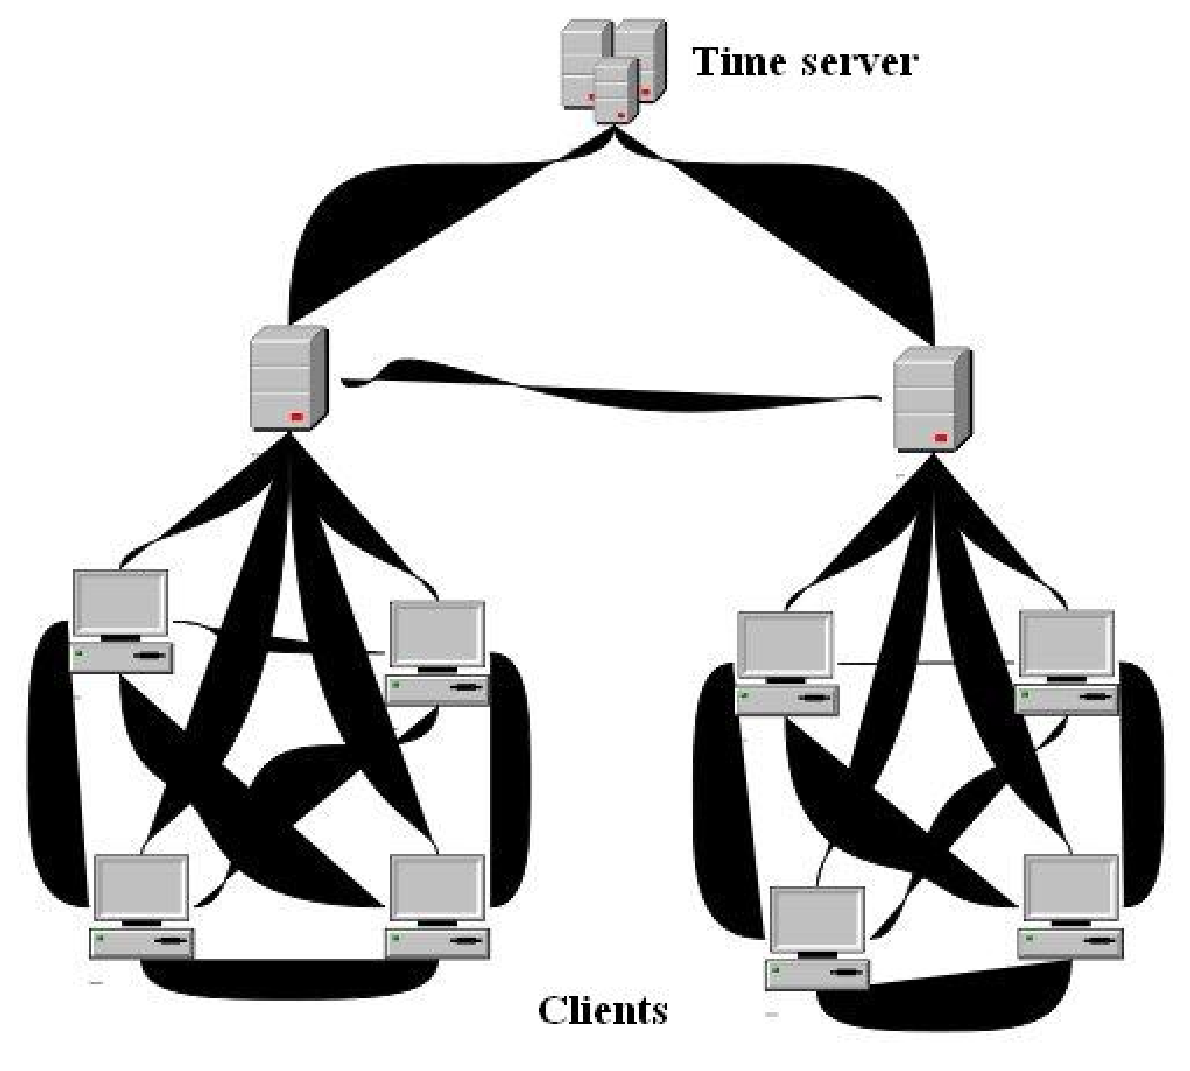
\includegraphics[width= 0.5 \textwidth]{ntp}
\caption{A simple NTP diagram} \label{ntp}
\end{figure}
\newline
The tiered nature of the NTP time distribution tree enables a user to choose the accuracy needed by selecting a level (stratum) within
the tree for machine placement. A time server placed higher in the tree (lower stratum number), provides a higher likelihood of
agreement with the \textit{UTC}\nomenclature{UTC}{Coordinated Universal Time} time standard.
\newline
Synchronization in traditional distributed systems takes a different kind of approach since there is no central authority to be referred
in case of time requests. Central nodes can be assigned as to play the role of a server as in the case of the centralized system.
But, most of the time, distributed systems, due to their unique properties, have no central command. Development of a synchronization
scheme that satisfies such requirements is challenging. The task becomes particularly daunting in WSNs, in light of their additional
domain requirements.
\section{\textbf{The need for a synchronized time}}
There are many reasons why a synchronized time is needed in a WSN. Some of them include data integration, TDMA scheduling, Target
Tracking and Localization. Two of the most common areas where synchronization is a necessity are described below.
\subsubsection{Data Integration}
Data collection is the main task of the sensor nodes, hence data gathering and integration is a crucial component. The signal processing literature sometimes refers to this as array processing; with heterogeneous sensors, it is often called \textit{data fusion}.
\begin{figure}
\centering
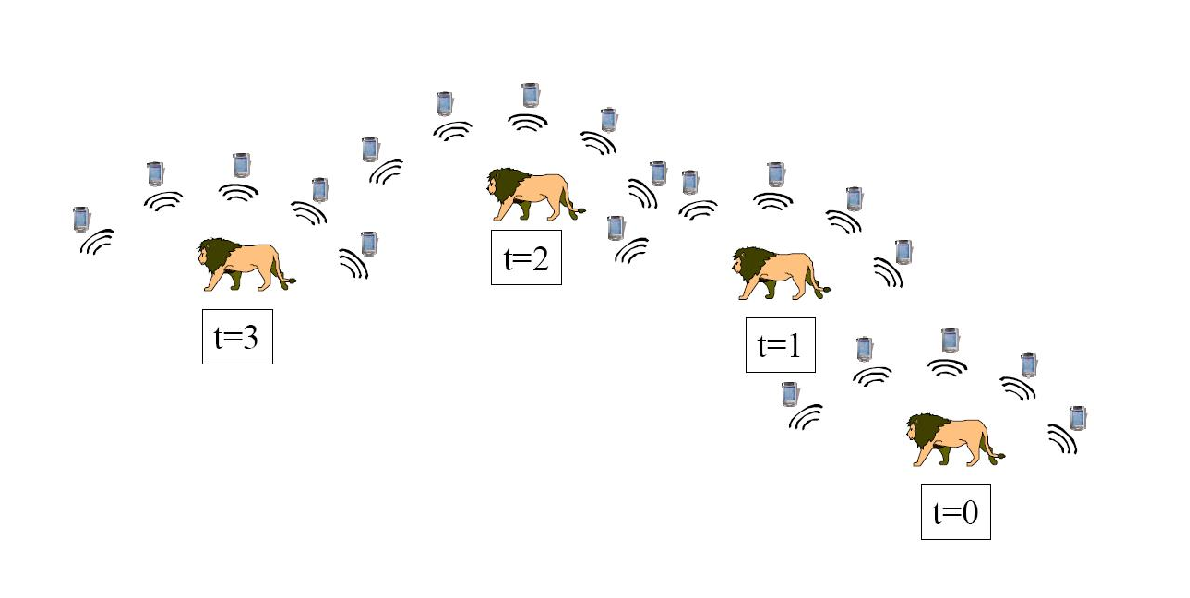
\includegraphics[width= 0.6\textwidth]{lions}
\caption{Tracking the movement of an object}
\label{lions}
\end{figure}
\newline
There are many applications which need data fusion such as signal enhancement (noise reduction), source localization, process control, and source coding. It would seem to be a natural match to implement such algorithms in distributed sensor networks, and there has been great interest in doing so. However, much of the extensive prior art in the field assumes centralized sensor fusion. That is, even if the sensors
gathering data are distributed, they are often assumed to be wired into a single processor. Centralized processing makes use of
implicit time synchronization. Sensor channels sampled by the same processor also share a common time base. Figure $\ref{lions}$ shows
one example of data fusion application. In order to locate the moving object, in this case the lion, nodes have to have a common
notion of time. Upon intergation, not only the location of the lion but also the time when the lion was spotted is necessary. So, having the same notion of time is important.
\subsubsection{TDMA schedule}
As previously stated, the WSN being developed at Chess uses a TDMA protocol for channel access, hence the reason for synchronization.
TDMA is a channel access method for shared medium (usually radio) networks. It allows several users to share the same frequency
channel by dividing the signal into different time slots. The users transmit in rapid succession, one after the other, each using his
own time slot. This allows multiple stations to share the same transmission medium while using only the part of its bandwidth they
require. Figure $\ref{tdmaframe}$ shows how a time frame is divided into receiver and transmitter slots. In the time frame, the active
slot is divided into one transmitting slot and many receiving slots. The number of visible slots, five, have been picked
arbitrarily in the figure and do not map to the selection in the simulation.
\begin{figure}
\centering
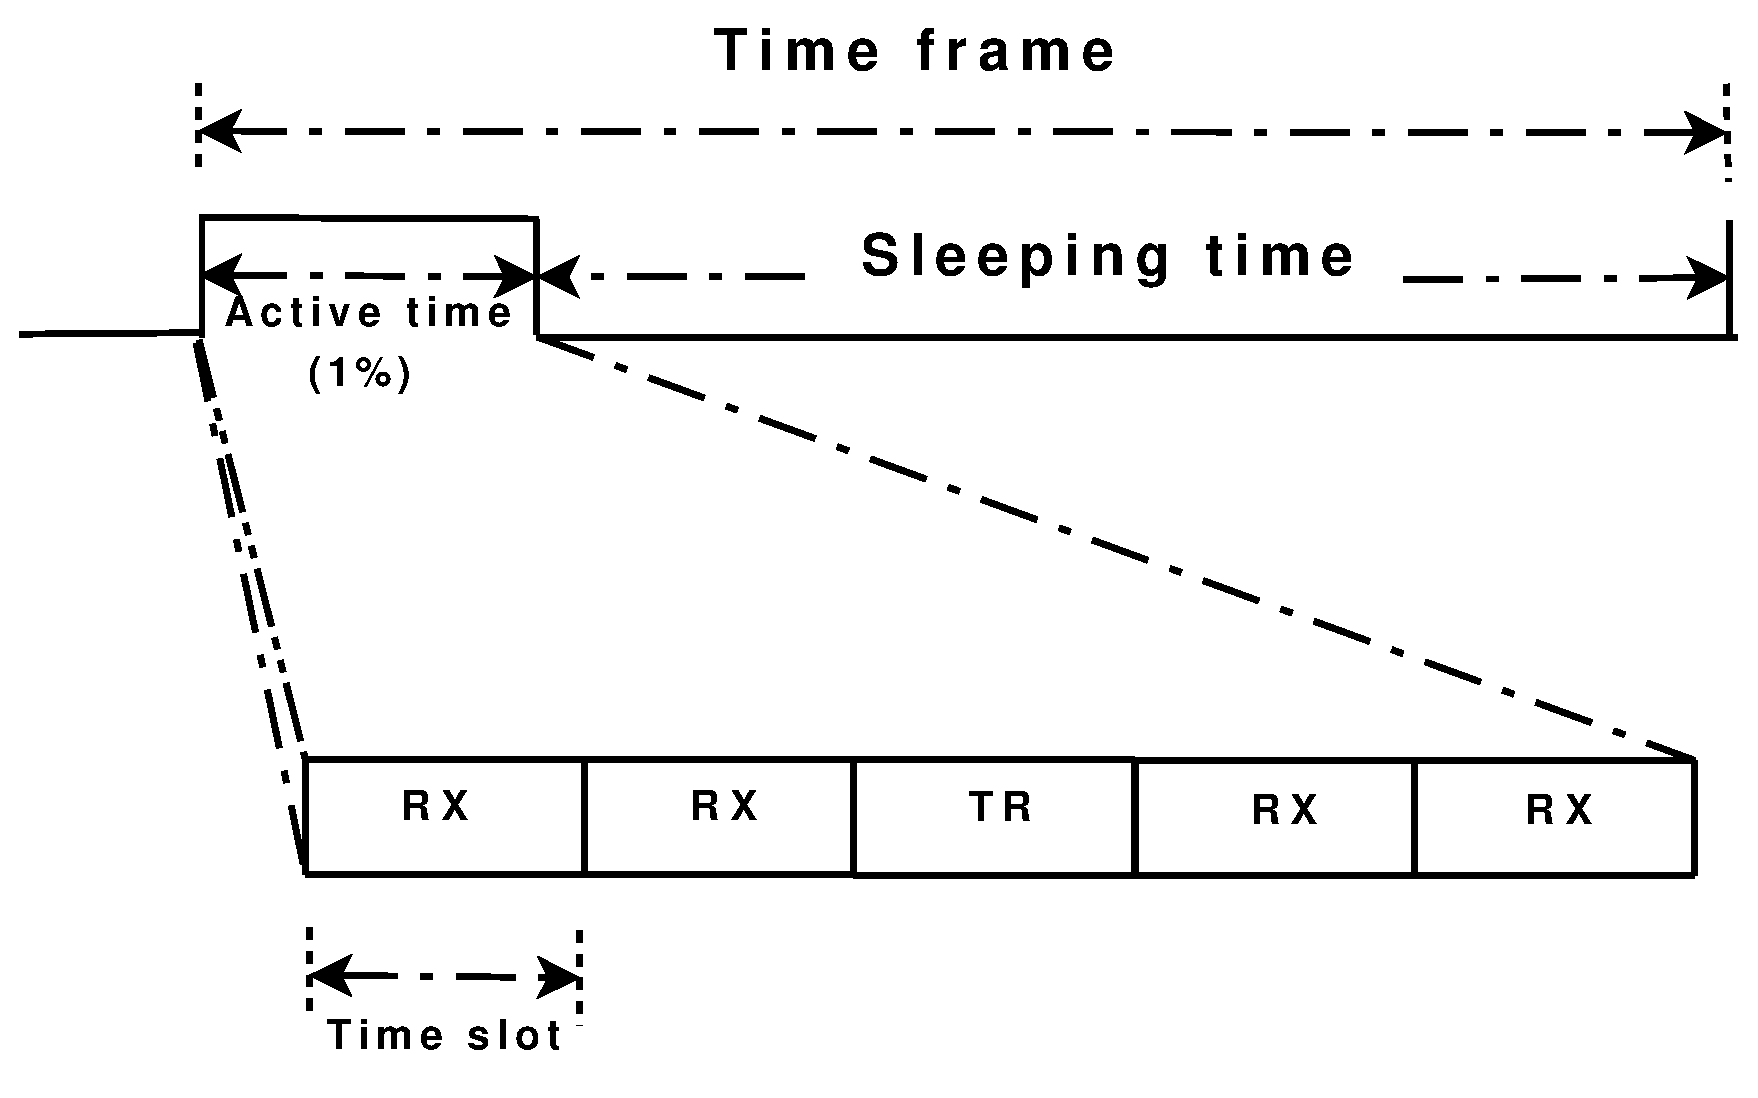
\includegraphics[width=0.6 \textwidth]{tdmaframe}
\caption{TDMA frame} \label{tdmaframe}
\end{figure}
\newline In this approach, nodes use time slots in order to communicate with each other. It is considered that two nodes have
their TDMA schedule synchronized when the numbers of the current time slot of any of the TDMA schedules involved are the same for any
given moment in time. The types of the slot may be different, TX or RX. To successfully initiate a network, the nodes has to be
synchronized and capable to send and receive messages. To establish a link between neighboring nodes, a particular node needs to know
the schedule of all its neighbors, which is the purpose of the slot allocation algorithm. The MAC protocol used in MyriaNed is the gMAC$\cite{pieter}$. The g in gMAC comes from Gossiping, which represents the gossip protocol implemented in the network layer$\cite{gossip}$.
\newline
Each neighbor has a different transmitting slot so that there will be no collision. Thus, a message transmitted should be in received in the receiving slot of the neighboring nodes. In order to have a seamless communication between the nodes, the synchronization of the frames is a necessary part of the MAC protocol. The processing element and other functions on a WSN operate on a local oscillator. Due to physical factors, the frequency of the oscillator has a drift. When no provisions are taken, it causes the nodes to run out of sync. Given that there is a certain error, the node will adjust its wake-up time at the end of the last receiver slot with the offset calculated with an algorithm. \newline
\begin{figure}
\centering
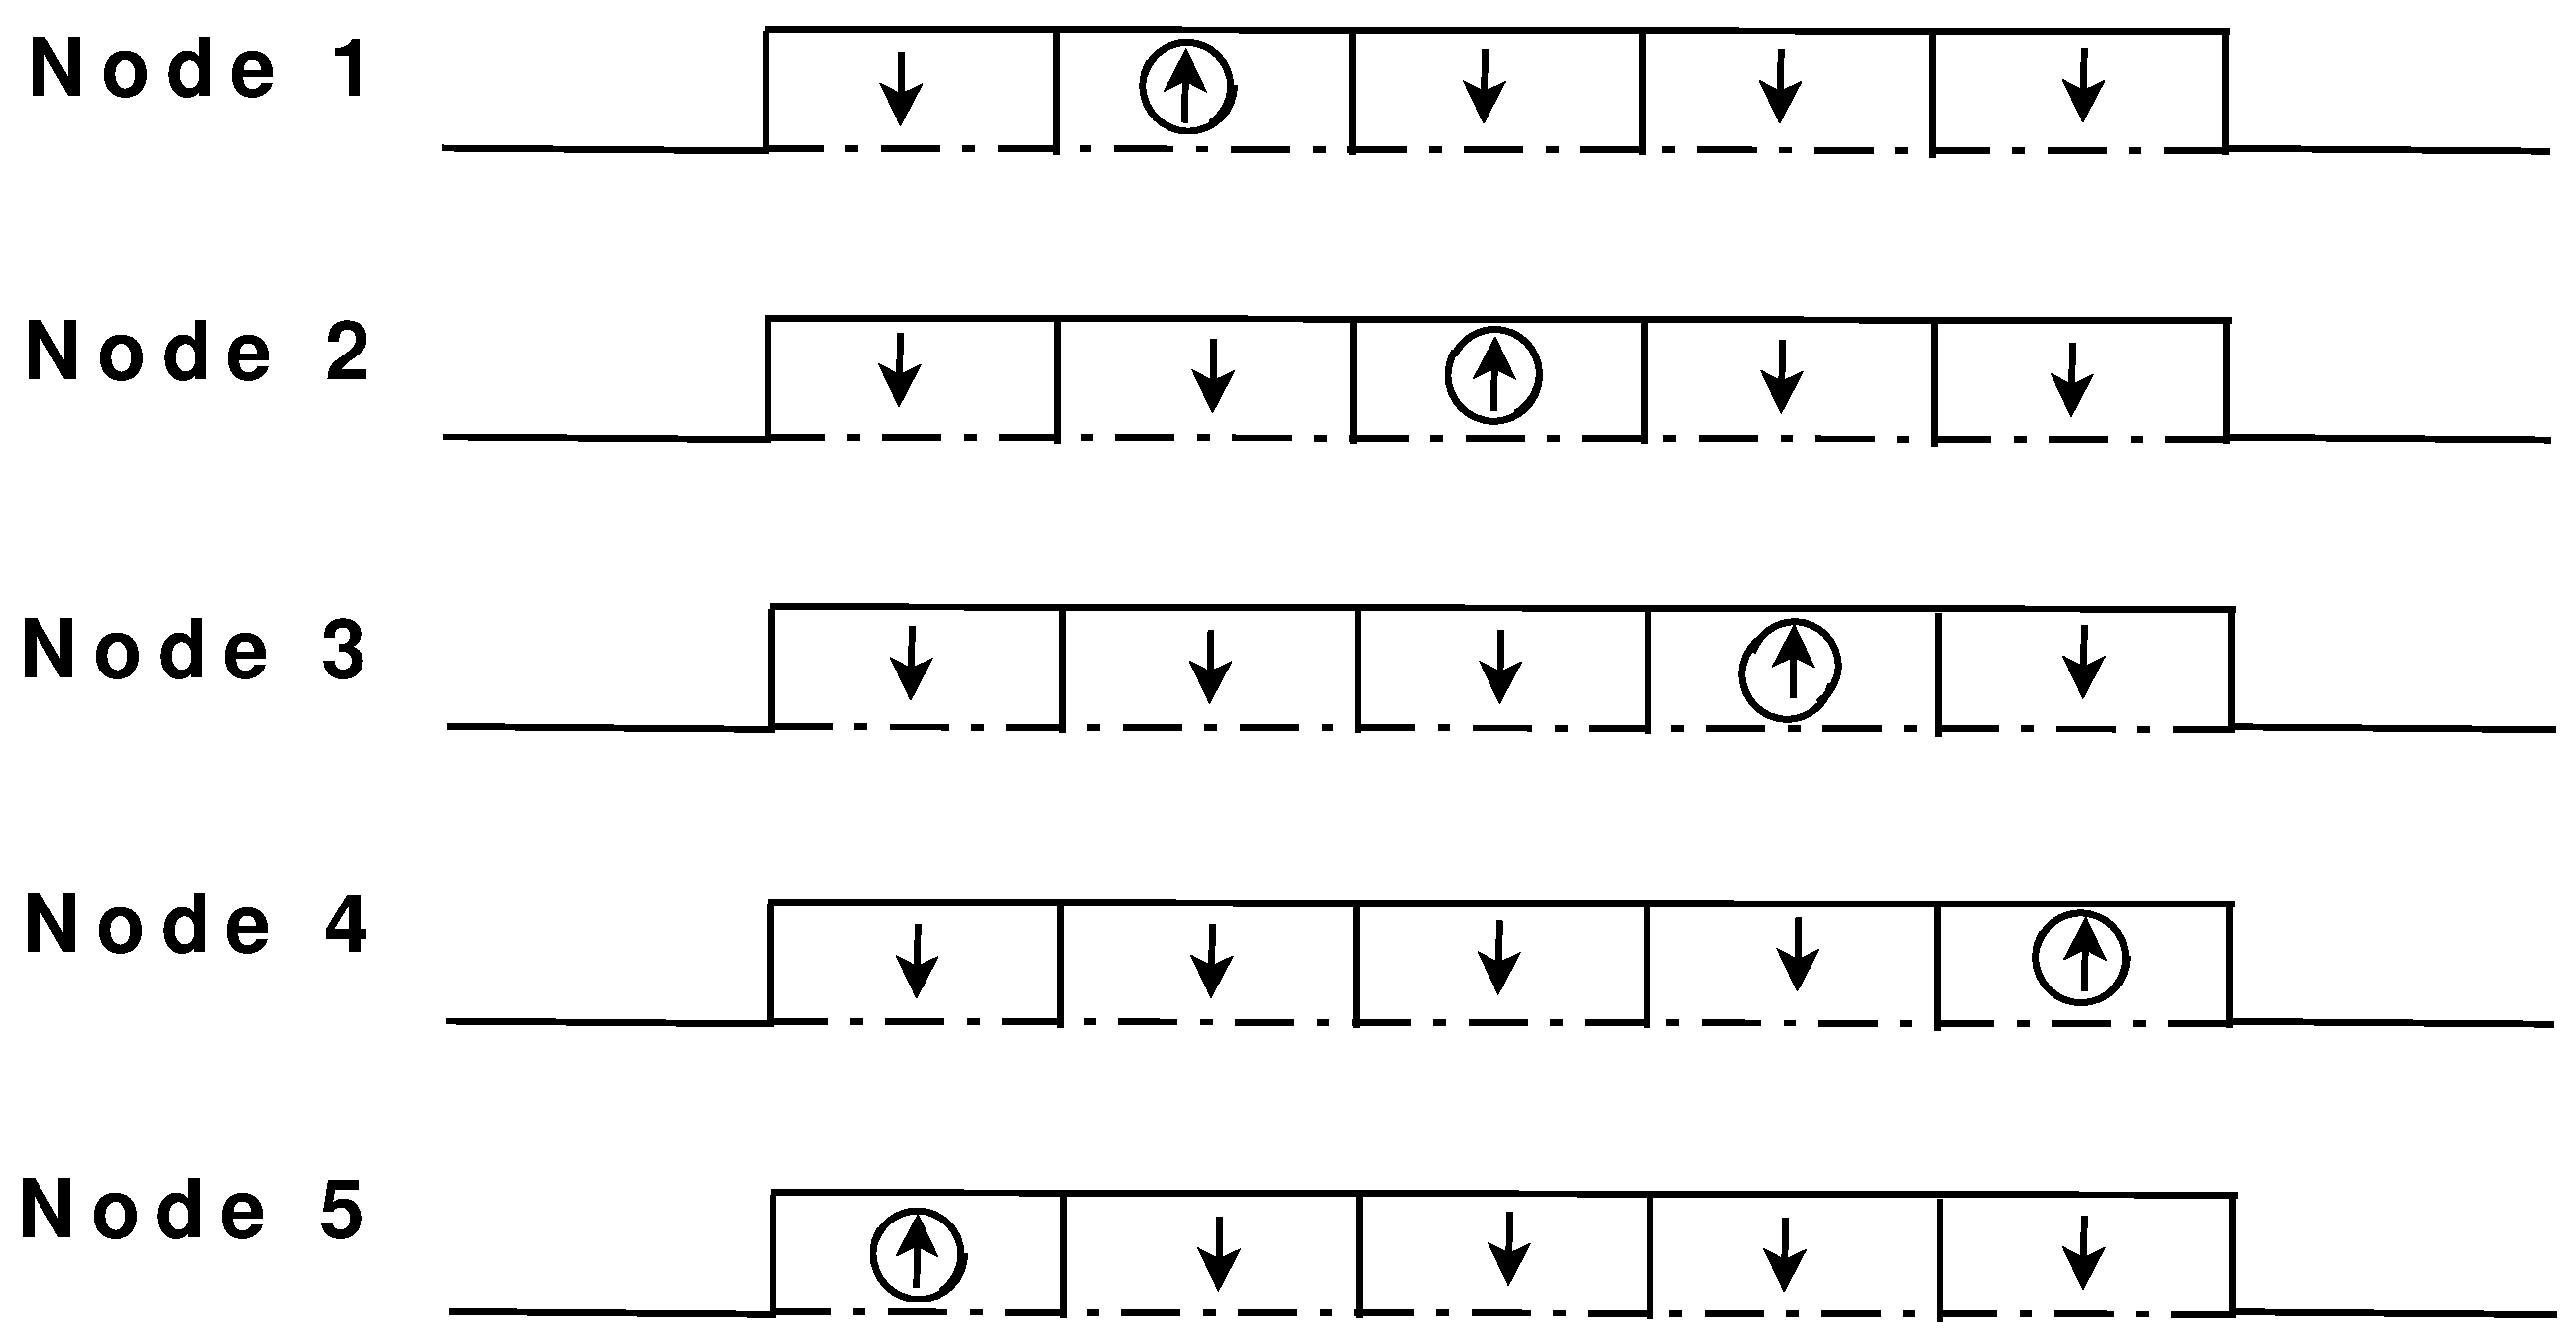
\includegraphics[width=0.6\textwidth]{tdmaschedule}
\caption{TDMA Channel access} \label{tdmasch}
\end{figure}
\newline
As it is implemented in WSN, the duty cycle is of prime importance due to the energy requirement of the nodes. A duty cycle is fixed length of time which is divided into a communication time and sleeping time (Figure $\ref{tdmasch}$). Major benefits can be achieved
by using this scheduled communication/sleeping protocol:
\begin{itemize}
\item Low duty cycles - a node can operate in low duty cycles, hence reducing the energy consumption of the nodes.
\item Efficiency in transmission - a sender can efficiently transmit a message to its neighbors by just waking up and sending exactly when a receiver is listening.
\item Efficiency in receiving - a receiver can schedule its own time intervals to receive a particular neighboring transmitter.
\end{itemize}
The communication quality of service is guaranteed by the gossiping layer probabilistic features. The scheduled communication/sleeping protocol, the multihop scheme and the rippling of the message through the network are best implemented using a TDMA scheme. Usually, this medium access scheme is best suited for the infrastructure mode where the base stations schedule the TDMA slots for each node (e.g. GSM). However, such structure is not used in WSN. The scheduling of the TDMA slots is made locally by reaching an agreement between direct neighbors.
\newline
Each node has a crystal oscillator that has a certain accuracy, which results in time drifts. This causes the TDMA time slot boundaries to drift when we compare two nodes with the same schedule. Hence, the need for synchronization is vital for the seamless communication of the nodes. But synchronization in WSNs is more challenging, which is explained in the next section.
\section{\textbf{Wireless Sensor Networks: Why different ?}}
Are traditional synchronization methods applicable in the case of WSNs? Many assumptions in the traditional schemes do not
hold in the case of WSNs. Some of these factors can be described as follows:
\begin{itemize}
\item \textbf{Energy Limitation}: Due to their small size and nature of applications which they are designed for, energy consumption is a major concern in a WSN. Nodes are mostly battery-powered and are expected to run for a number of years before they run out of power. An energy efficient method is a requirement for WSNs.
\item \textbf{Dynamic Nature of the Network}: In a centralized system, the topology remains more or less static even if there are physical
dynamics involved  in some centralized systems like \textit{GSM} \nomenclature{GSM}{Global System for Mobile communications}. In a WSN, network dynamics
results from various factors like mobility of nodes, node failures, environmental obstructions etc., which prevents simple static
configurations. Hierarchical structures might get nodes poorly synchronized, and nodes might not be connected when they need
synchronization the most.
\item \textbf{Diverse Applications}: WSNs are used for a variety of applications, which can have totally different needs as far as synchronization is concerned. For example, localization applications need a short-lived but highly
precise synchronization, while target tracking applications can tolerate a little lower precision, but want the synchronization to
last longer. Some applications might need a global timescale while some others can work with a local timescale. And while a few require
absolute or real time as reference, for others, a relative notion of time is enough.
\item \textbf{Cost of the Nodes}: Sensor nodes are very small in size and must be cheap cost wise since they are implemented in large
numbers. Now, we can obtain very good synchronization with \textit{GPS}\nomenclature{GPS}{Global Positioning System} receivers, but it will be unreasonable to put an expensive and energy-hungry GPS receivers on a sensor node. This is too costly.
\end{itemize}
All the above factors make the problem of time synchronization more challenging in case of WSNs. Keeping this in mind, we can formulate
some design requirements, in general, for WSN frame synchronization. These complications are startling to look for a new arena for the synchronization of WSNs.
\chapter{\textbf{Problem Formulation}}
\section{\textbf{Sources of synchronization error}}
The first step in designing any time-synchronization algorithm would be to understand why and where it is required. The different factors
which give rise to errors in clocks of nodes or in synchronization algorithm can be divided into two main categories:
\begin{enumerate}
\item \textbf{Oscillator Characteristics}: The sensor node's clocks run on very cheap oscillators. The following two characteristics are the main sources of errors between the clocks of two different nodes.
         \begin{description}
         \item \emph{\textbf{Accuracy}}: This is a measure of difference between oscillators expected (ideal) frequency and actual frequency. It is also called as the calibration tolerance of the clock; its maximum is specified by the manufacturer.
         \item \emph{\textbf{Stability}}: This is the oscillator's tendency to stay at the same frequency over time. There can be short-term instability due to environmental effects, supply voltage, long-term instability due to temperature effects and crystal aging.
      \end{description}
\item \textbf{Hardware and Environmental factors}: The non-determinism in the message delivery latency is a major source of error in any synchronization algorithm, when applied into real sensor networks. This can be categorized in four type of delays:
      \begin{description}
         \item \emph{\textbf{Send Time}}: The time spent at the Sender to build the message, i.e. the time duration between generating the message and injecting it into the network.
         \item \emph{\textbf{Access Time}}: Delay occurred while waiting for access to the transmit channel.
         \item \emph{\textbf{Propagation Time}}: Time required for the message to travel from sender to receiver.
         \item \emph{\textbf{Receive Time}}: Time needed for processing at the receivers network interface.
      \end{description}
\end{enumerate}
      All the above factors result in following errors between the clocks of two nodes:
\begin{description}
\item \textbf{Phase error}: The oscillators of any two nodes can be out of phase at any given time, resulting into different time on both clocks. There can be some initial difference between nodes' clocks at the start of a synchronization procedure. Phase error is an instantaneous metric. It describes how far apart are the clocks at a given time.
\item \textbf{Frequency error}: Frequency error, in contrast, measures the difference in the clock rates. This metric is important because it predicts the growth of phase error over time. That is, if clocks are perfectly synchronized now, at what rate are they drifting apart? How well will they be synchronized in 60 seconds?
\item \textbf{Clock drift}: It is not just that the clocks are running at different rates, but even the frequency of each clock does not stay constant over a period of time. Clock drift arises from the instability of oscillators, because clocks drift from their initial frequency. For instance, if each clock drifts at a rate of $\theta$ msec/sec, then maximum relative drift between two clocks can be 2$\theta$ msec/sec.
\end{description}
Even if two clocks are assumed to have the same frequency and no drift, the above mentioned delays in the network result in phase
error between two clocks. This is because when the message from the sender reaches a receiver, the receiver adjusts its clock according
to the received message. But the sender's clock changes in the mean time due to network delays. For a network of nodes, delays give rise
to errors in accuracy from an ideal clocks, and dispersion amongst their clocks.
\section{\textbf{Clock and Frequency standards}}
The quality of a clock usually amounts to its frequency stability which is the ability of its frequency standard to emit
events at a constant frequency over time. The absolute value of the frequency compared to the desired value or, its frequency accuracy
is also important. Calibration can easily compensate for an inaccurate but stable clock.
\newline As per our motive to a synchronized clock, clocks are very important in this research: the error bound achieved by a clock
synchronization method is linked to both the error inherent in the method itself, and the stability of the clocks' frequency. In fact,
to some extent, the two are interchangeable. Stable clocks can compensate for a synchronization channel between them that is prone
to large but unbiased errors: many synchronization events can be averaged over a long time. Similarly, a precise synchronization
channel can compensate for a poor-stability crystal oscillator whereas frequent synchronization minimizes the time in-between when the
clock is left to fend for itself.
\newline
Many types of frequency standards exist. In general, as their stability and accuracy increase, so do their power requirements,
size, and cost, all of which are important in WSNs. Most commonly found in computer clocks are quartz crystal oscillators,
characterized by $\cite{6}$. Quartz crystals are attractive because they are inexpensive, small, use little power, and perform
surprisingly well despite their low resource requirements. The frequency generated by a quartz oscillator is affected by a number
of environmental factors: the voltage applied to it, the ambient temperature, acceleration in space (e.g., shock or attitude
changes), magnetic fields, and so forth. More subtle effects as the oscillator ages also cause longer-term frequency changes. The
inexpensive oscillators commonly found in computers have a nominal frequency accuracy on the order of between $10^4$ to $10^6$ that is,
two similar but uncalibrated oscillators will drift apart between 1 and 100 microseconds every second, or, between about 0.1 and 10
seconds per day $\cite{6}$ $\cite{7}$. However, their frequency stability is significantly better with a change in frequency of one
part in $10^9$ to $10^{11}$ when averaged over several seconds or more. In our implementation, a 32 kHz crystal clock $\cite{18}$
$\cite{19}$  is used in the MyriaNode$\footnote{MyriaNode is the sensor node which is built for the project MyriaNed.}$.
\section{\textbf{Clock Time and Delay}}
In this section, we will see the clock time and its expression. From the definition of frequency:
\begin{equation}
f = d\phi/dt \label{freq_defn} ,
\end{equation}
and integrating both sides over time,
 \begin{equation}
\phi =\int f(t)dt ,
 \end{equation}
where $f$ is frequency, $\phi$ is phase, and $t$ is time.\newline
Thus, the clock time is described as
\begin{equation}
C(t) = \frac{1}{f_o}\int_{t_o}^{t} {f(\tau)d\tau} + C(t_o) ,
\label{clock}
\end{equation}
where $f(\tau)$ is the frequency of the clock, $f_o$ is the nominal frequency of the crystal oscillator and $t_o$ is the start time of
the node. The exact clock drift is hard to predict because it depends on environmental influences (such as temperature, pressure
and power voltage). One can usually assume that the clock drift of a computer clock doesn't exceed a maximum value $\rho$ . This means
that it can be assumed
\begin{equation}
1-\rho \leq \frac{dC(t)}{dt} \leq 1+\rho ,
\end{equation}
where $\rho$\nomenclature{$\rho$}{Maximum clock drift} represents the maximum clock drift. Figure $\ref{clocktime}$ shows the relationship between clock time and absolute time for different drift rate $\rho$.
\begin{figure}
\centering
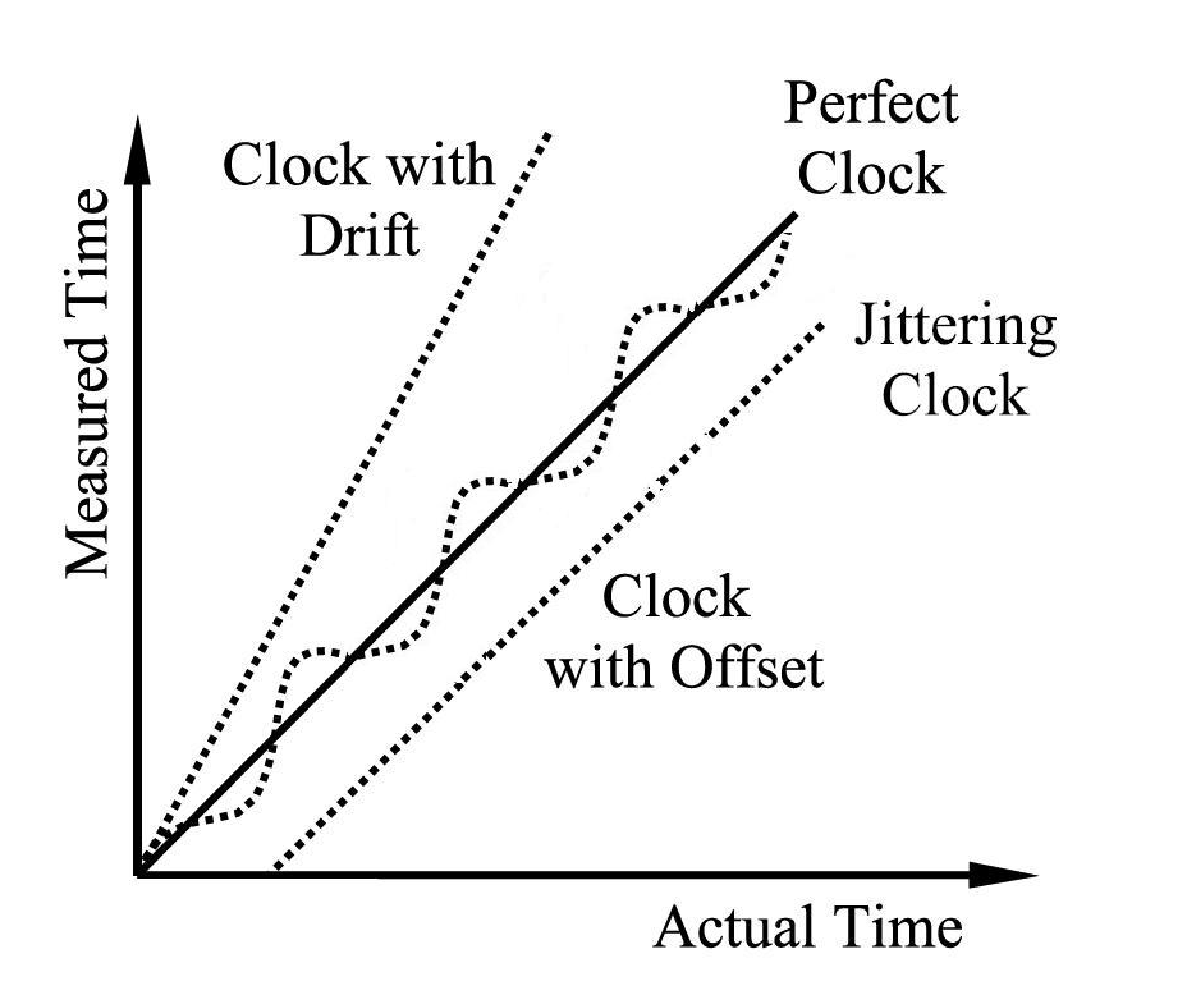
\includegraphics[width=0.5 \textwidth]{actualvsmeasuredtime}
\caption{Measured time versus absolute time} \label{clocktime}
\end{figure}
\newline
A typical value for $\rho$ achievable with our crystal clock is $30ppm$ which means that the clock drifts away from real time by no more than 30 seconds in ten days, which is still a significant value. Note that different clocks have different maximum clock drift values
$\rho$.\newline The frequency of the clock is dependent on many factors and is given as
\begin{equation}
f_i(t) = f_o + \Delta f + a(t-t_o) + \Delta f_e(t-t_o) + f_r(t)
\label{frequency}
\end{equation}
where \newline $t_o$ = the start time of the clock, \newline $a$ = aging factor,  \newline $f_o$ = nominal frequency, \newline $\Delta
f$ = calibration error,\newline $f_r(t)$ = frequency instability (noise) term, \newline $\Delta f_e$ = frequency error which occurs
due to outside factors such as temperature and voltage instability.
\newline
The nominal frequency is the ideal frequency at which the oscillator is supposed to run. \newline Hence, all the above factors affect the value of $\rho$.
From ($\ref{clock}$) and ($\ref{frequency}$), we get
\begin{equation}
C_i(t) - C_i(t_o) = \frac{1}{f_o} \int^{t}_{t_o}f_i(\tau)d\tau ,
\end{equation}
\begin{eqnarray*}
C_i(t) - C_i(t_o) & = & \frac{1}{f_o} \int^{t}_{t_o}{[f_o + \Delta f + a(\tau-t_o)  } \\
 &  & {} + \Delta f_e(\tau-t_o) + f_r(\tau)]d\tau ,
\label{fasika}
\end{eqnarray*}
\begin{eqnarray*}
C_i(t) & = & C_i(t_o) + (t-t_o) +\frac{\Delta f}{f_o}(t-t_o) \\
& & + \frac{a}{2f_o}(t-t_o)^2 + \frac{\Delta f_e}{2f_o}(t-t_o)^2 +
\frac{1}{f_o}\int^{t}_{t_o}{f_r(\tau)d\tau} .
\end{eqnarray*}
The amplitude of the short term variations due to noise (clock
jitter) is small enough that they do not cause the clock to
accelerate or decelerate in a very large amount in the long run. But
the environmental term, primarily due to temperature, and the error
due to calibration can be significant. Thus, the phase or time
offset between two clocks at any given time results from: a
combination of initial phase offset, frequency bias, calibration
error, frequency drift and the environmental terms. As more time
passes from the synchronization point, the drift and environmental
terms become more significant. The resulting expression is used to
model the clock drift of an oscillator.\newline \textbf{Definition}
: A clock cycle (clk)(\nomenclature{\textit{clk}}{A clock cycle} )
is the time between two adjacent pulses of the oscillator. The
number of these pulses per second is known as the clock speed,
measured in kHz, MHz.
\section{\textbf{Median algorithm and the setback}} In this section, we will see the Median algorithm which is
currently implemented in the MyriaNode. The algorithm is described
as follows:
\begin{enumerate}
\item Nodes broadcast packets.
\item Each receiver records the time that the packet is received according to the local clock.
\item Each receiver $i$ computes its phase error to any other node j in the neighborhood,
\begin{equation}
\Delta t_{ij}^{(n)} = t_i^{(n)} - t_j^{(n)} ,
\end{equation}
where $t_i$ is the wake-up time of node $i$ and $t_j$ is the wake-up
time of node $j$ at the $n^{th}$ period.
\item Receivers compute the median of the phase errors,
\begin{equation}
\xi_i^{(n)} = m(\Delta t_{ij}^{(n)}) , \forall j
\end{equation}
\item Receivers adjust their wake-up time by the computed offset value,
\begin{equation}
t_{i}^{(n+1)} = t_i^{(n)} + T_i^{(n)} - k\xi_i^{(n)},
\end{equation}
\end{enumerate}
\begin{figure}
\centering
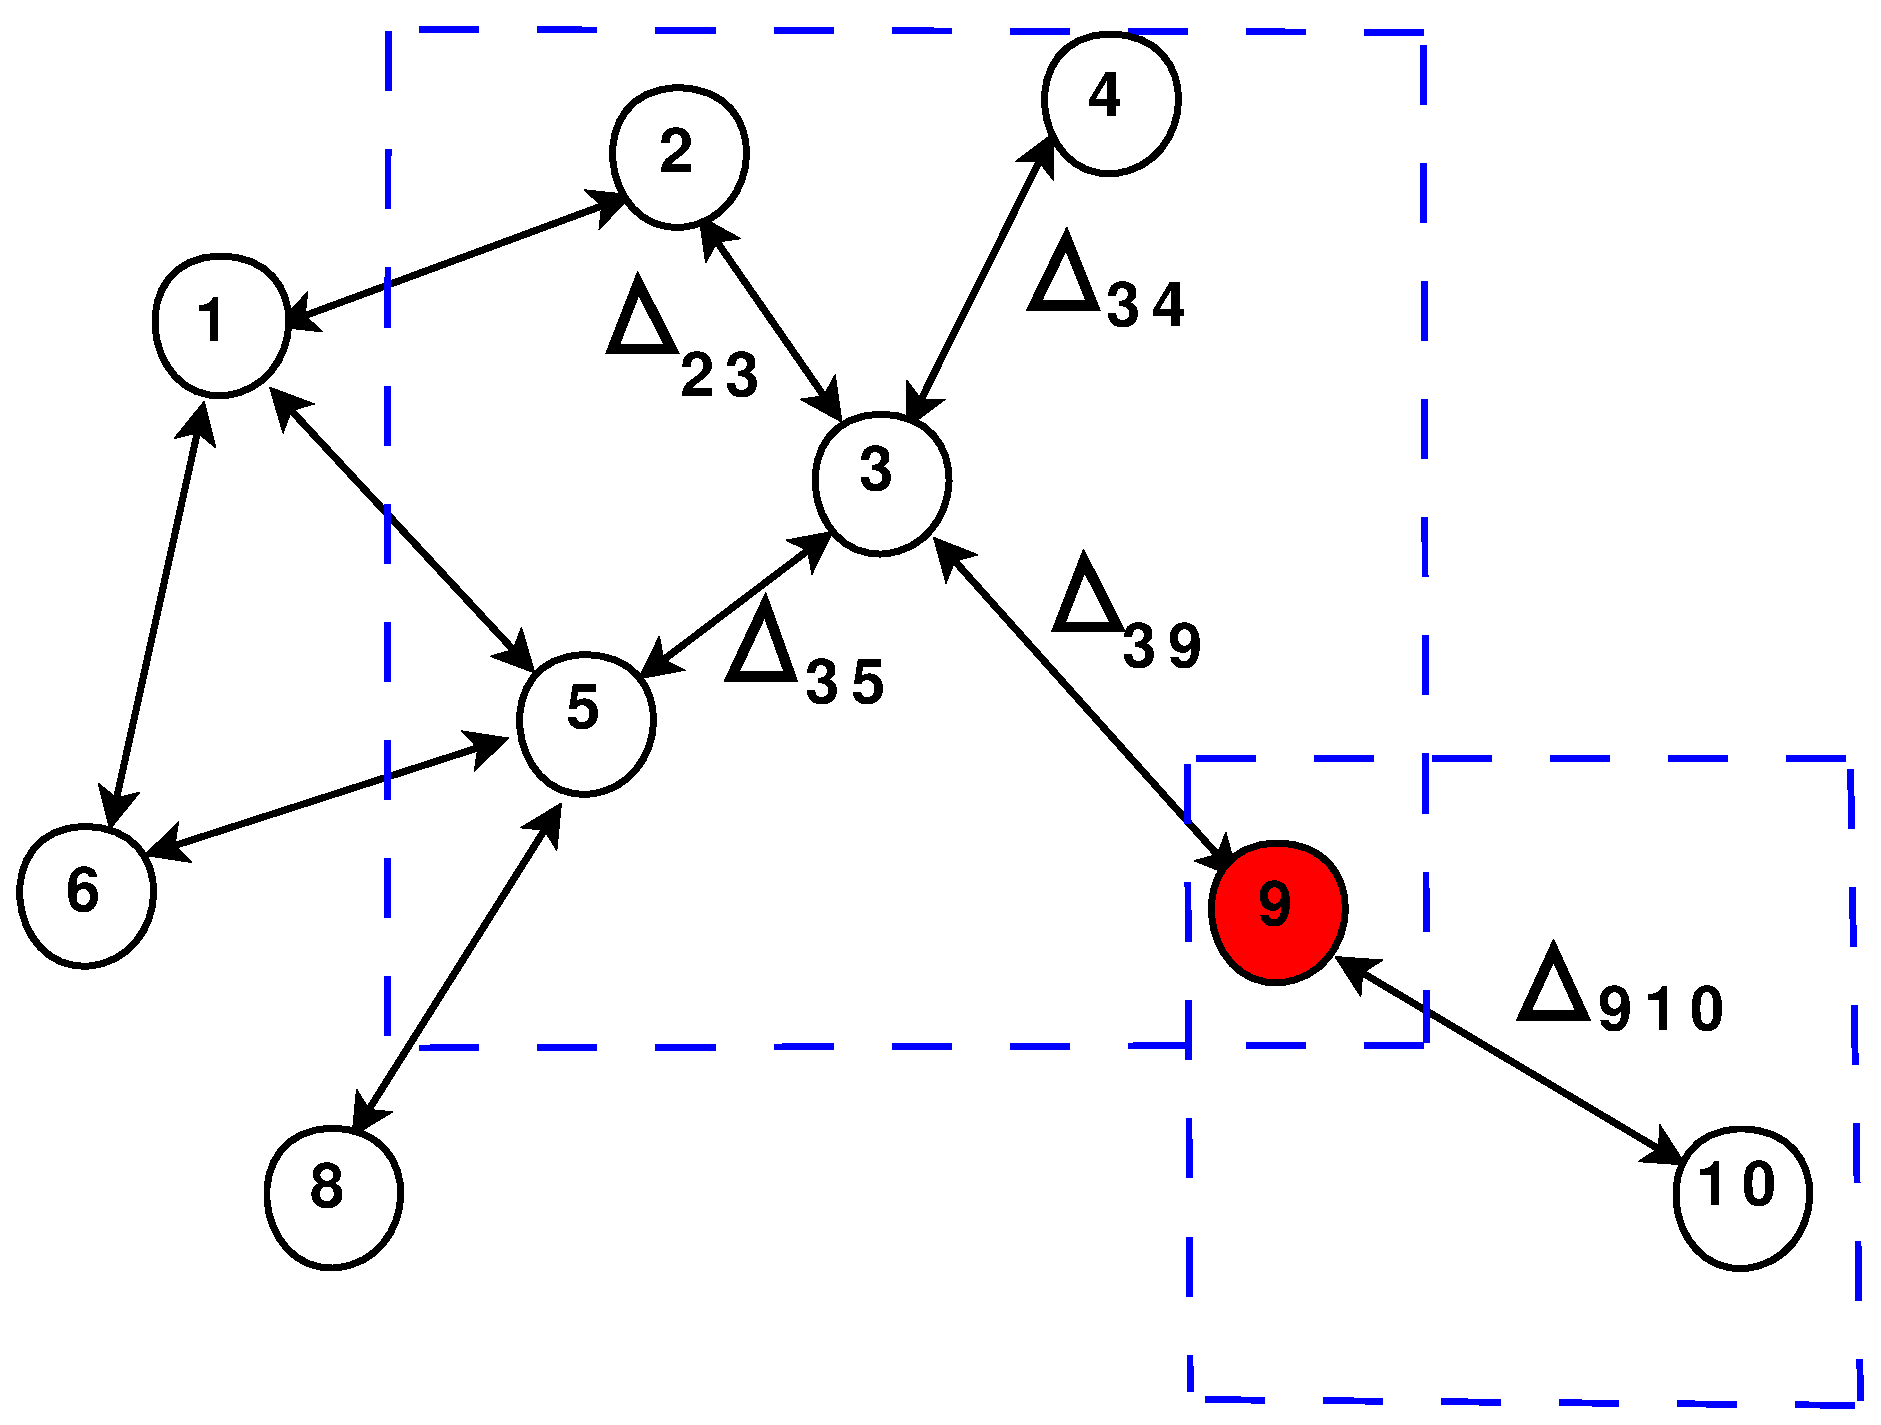
\includegraphics[width=0.6 \textwidth]{node_field}
\caption{A WSN scenario} \label{wsn}
\end{figure}
where $k$ is the \textit{gain factor}. \newline
By multiplying the median with a gain factor, i.e. $k\xi_i^{(n)}$, the output can be adjusted for better performance. Hence a gain factor could be added to ensure better precision of the synchronization error.
\newline As per the application of Median, there are setbacks on its implementation. In some test-cases, the algorithm fails to converge or stays unsynchronized for a certain period of time. This results in a  communication disruption in places where synchronization is essential.
\newline A typical scenario is presented where the Median algorithm takes a longer time to achieve synchronization. In Figure
$\ref{wsn}$, a distribution of wireless sensor nodes is shown. Node 10 joins the stable network communication through Node 9. Assume Node
9 belongs to two broadcast domains, Node 3's and Node 10's. Thus, upon the application of the median algorithm, the node tends to
adjust its wake-up time with the median of the offsets from its neighbors, Node 3 and Node 10. Adjusting the wake-up time, we get
the offset to be
\begin{equation}
\xi_9 = \frac{\Delta t_{910} + \Delta t_{39}}{2}.
\end{equation}
With Node 10 being isolated from the well established network, it has a major drift from the other nodes. Being in sync
with the other nodes, Node 9 will drift away from the network after its adjustment with the Node 10. It will take more time to
synchronize with the network again. Hence, the performance of the median algorithm decreases with the dynamic nature of the network.
Figure $\ref{fasik}$ shows the state of the network after the synchronization using the Median. Node 9 has drifted away from the
networks in order to incorporate the effect of Node 10.
\begin{figure}
\centering
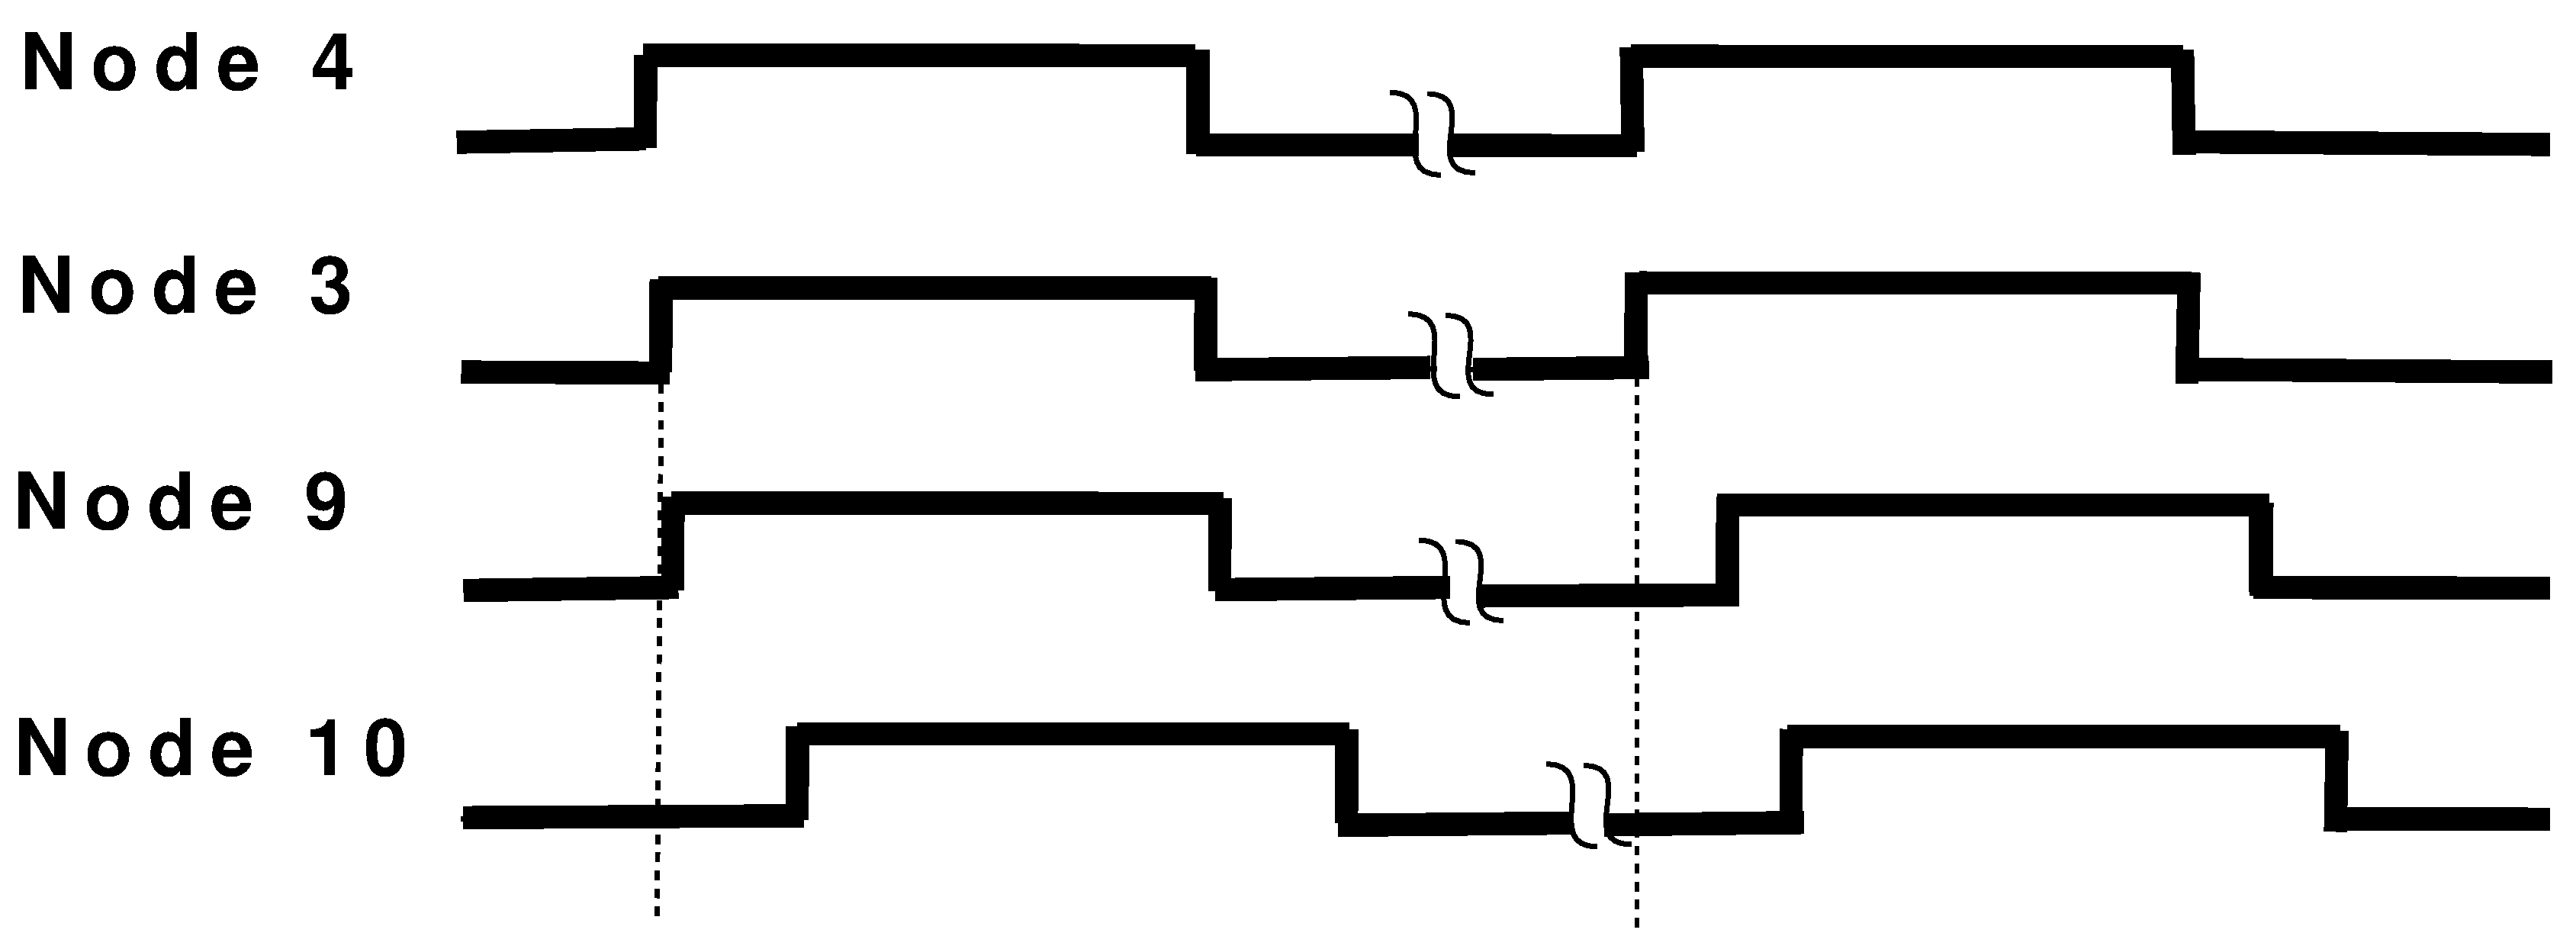
\includegraphics[width= 0.6\textwidth]{offsetpic}
\caption{Using median for phase error correction} \label{fasik}
\end{figure}
\newline
So, in order to address this problem, three algorithms are developed to realize an energy-efficient, more precise and simple frame synchronization.
\section{\textbf{Performance metrics of a synchronization protocol}}
The synchronization protocols can be decomposed into four conceptual building blocks$cite{11}$. It is shown in Figure
$\ref{block}$.
\begin{figure}
 \centering
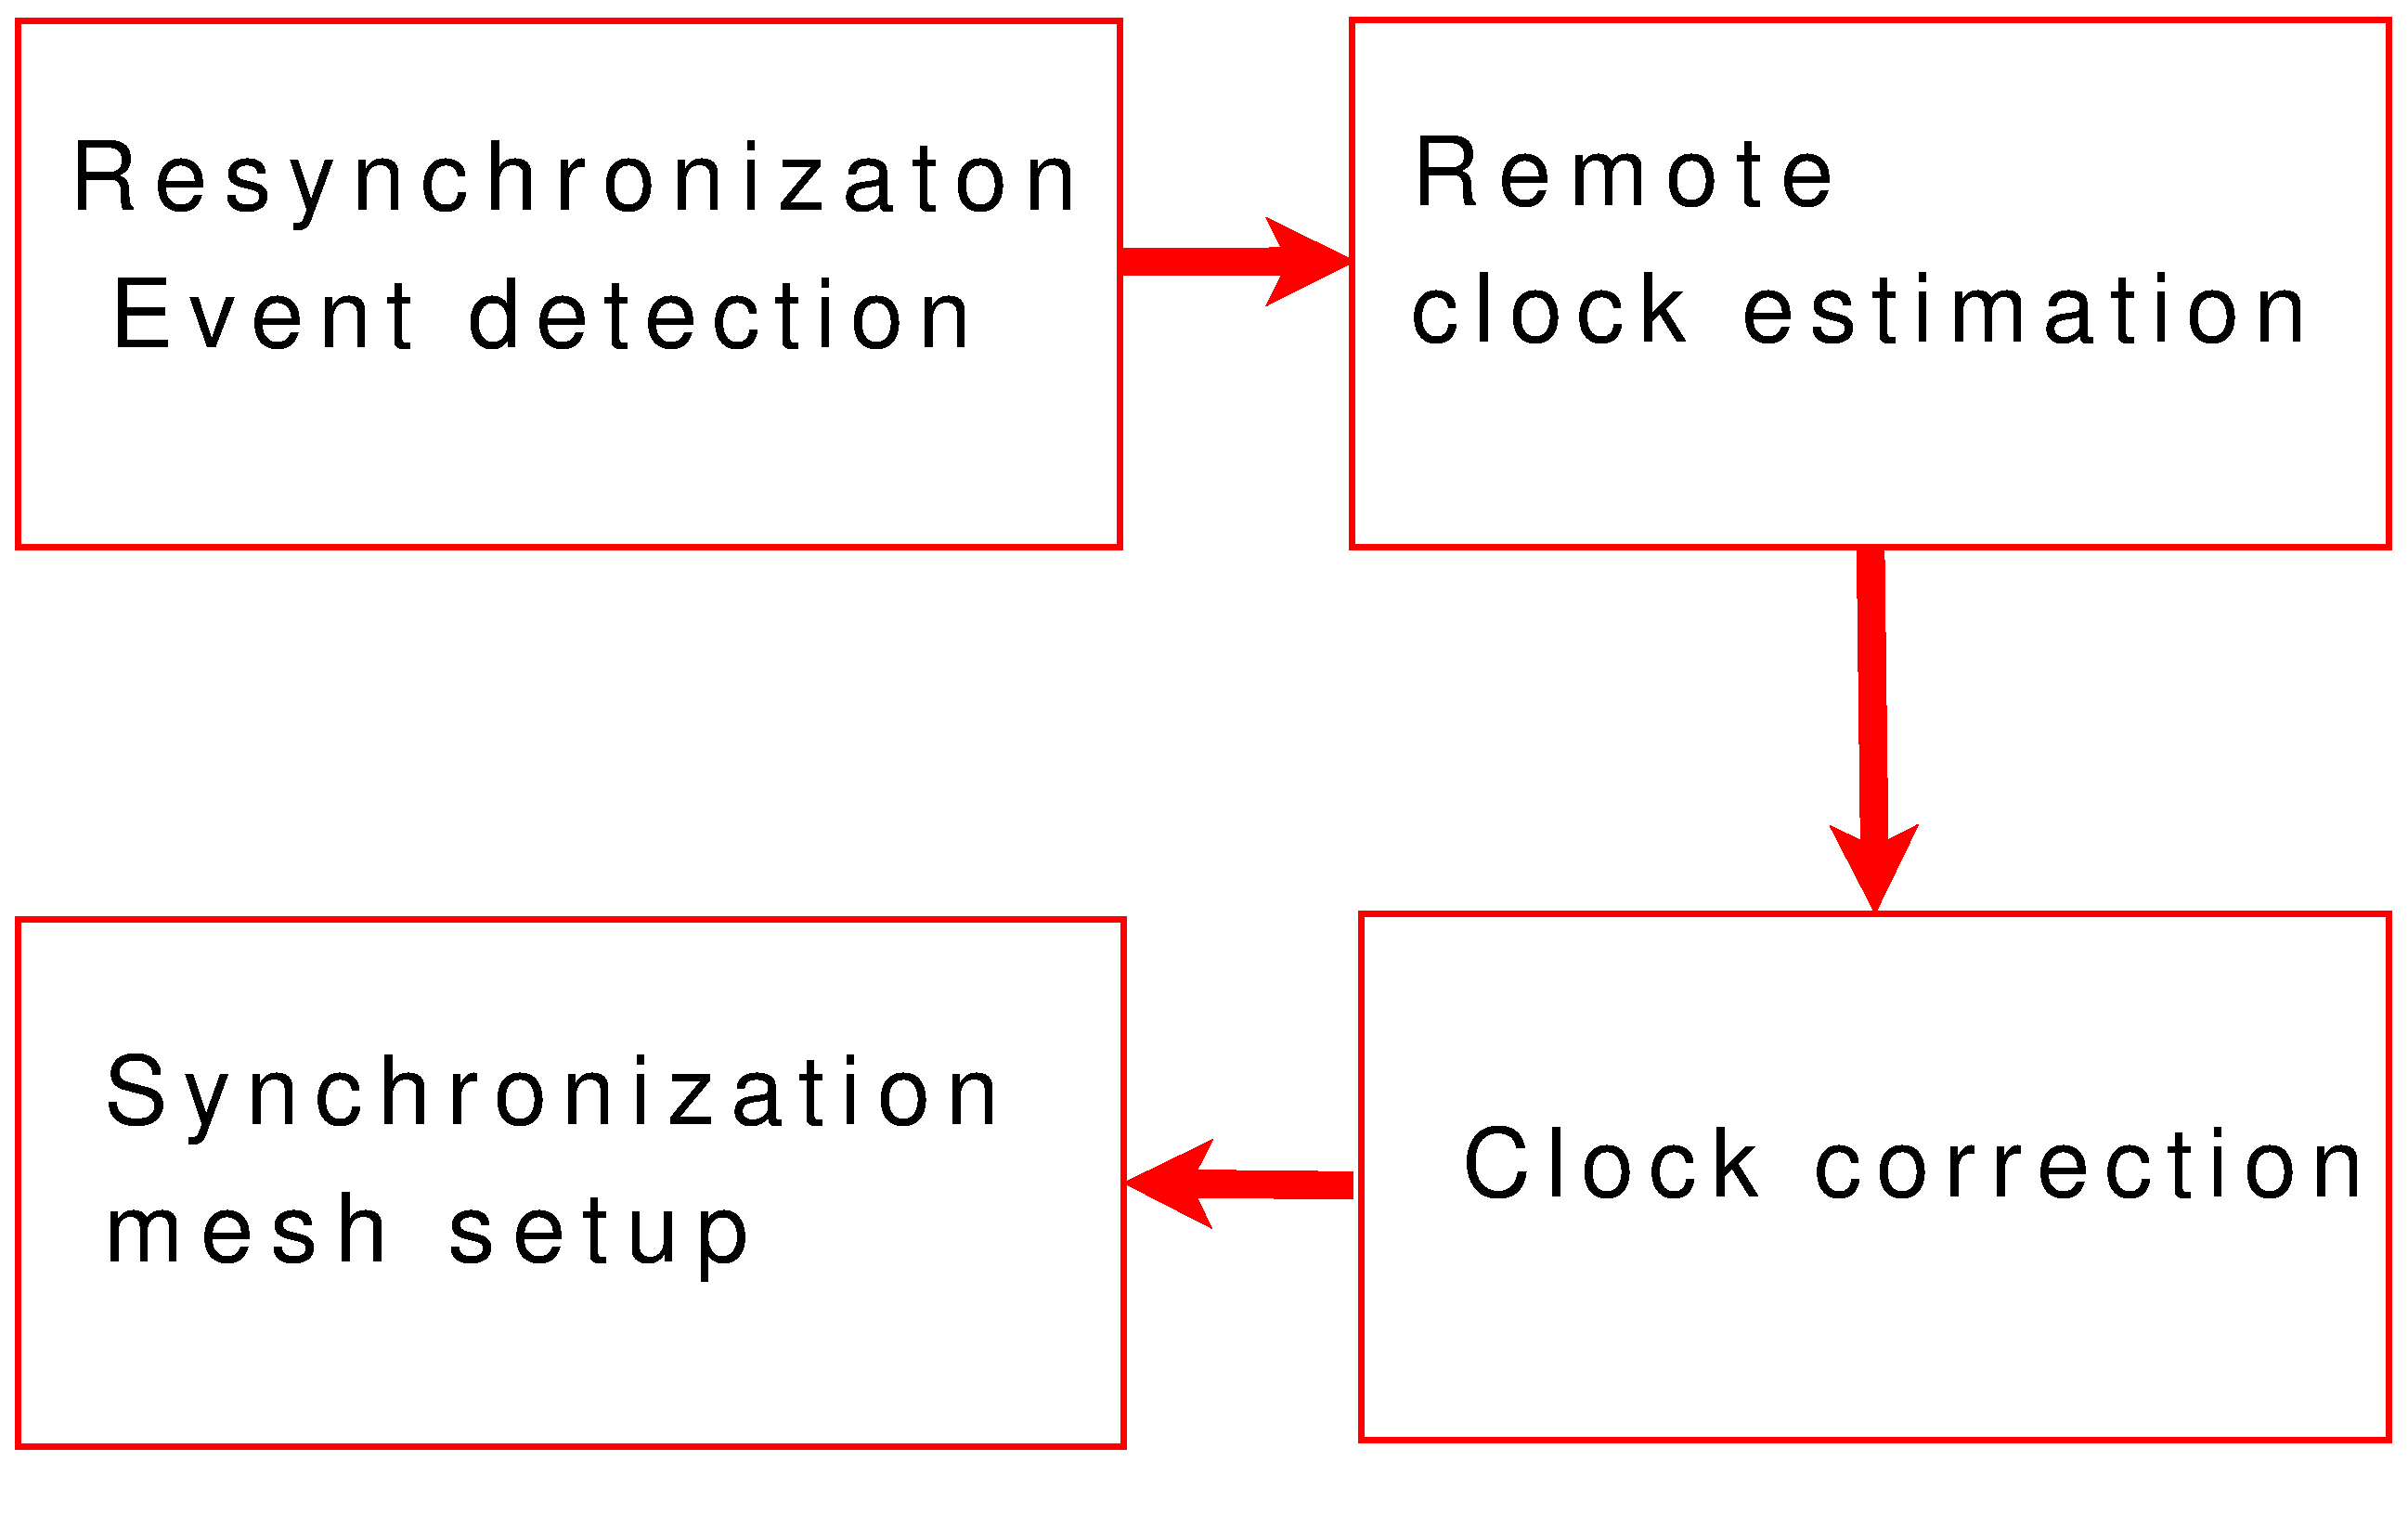
\includegraphics[width= 0.6 \textwidth]{buildingblock}
\caption{Building block of a time synchronization algorithm}
\label{block}
\end{figure}
\begin{itemize}
\item The resynchronization event detection block identifies the points in time where resynchronization is triggered. A single synchronization process is called a round. If rounds can overlap in time, sequence numbers are needed to distinguish them and to let a node ignore all but the newest resynchronization rounds.
\item The remote clock estimation block acquires clock values from remote nodes/remote clocks.
\item The clock correction block computes adjustments of the local clock based on the results of the remote clock estimating block.
\item The synchronization mesh setup block determines which nodes synchronize with each other in a multihop network. In fully connected networks, this block is trivial.
\end{itemize}
There are different metrics in which a synchronization algorithm can be measured. Some of the parameters are discussed below.
\subsection{\textbf{Precision}}
Deterministic algorithms guarantee absolute upper bounds on the synchronization error between the nodes or with respect to external time source. In this case, the maximum synchronization error between a node and real time or between two nodes is interesting; for stochastic algorithms (which can only give stochastic bounds in the sense that that synchronization error is with some probability smaller than a prescribed bound), the mean error, the error variance or some other quantity is relevant.
\subsection{\textbf{Energy costs}}
The energy costs of a time synchronization protocol depend on several factors: the number of packets exchanged in one round of the algorithm, the amount of computation needed to process the packets, and the required synchronization frequency.
\subsection{\textbf{Memory requirement}}
To estimate drift rates, a history of previous time synchronization packets is needed. In general, a longer history allows for more accurate estimates at the cost of increased memory consumption.
\subsection{\textbf{Fault tolerance}}
How well can the algorithm cope with failing nodes, with error-prone and time-variable communication links, or even with network partitions? Can the algorithm handle mobility?
\chapter{\textbf{Synchronicity protocol}}
\section{\textbf{Requirements of the Algorithm for MyriaNed}}
\subsubsection{\textbf{Precise synchronization}}
Synchronization cab be of two types: Course and Precise synchronization. Course synchronization is implemented when a node is joining in the network. After a newly joining node listened the synchronization information sent by the other nodes in the network, it adjusts its time slot reference to the time when it detects the synchronization information, which includes the propagation delay. Precise synchronization is implemented when a node has already joined in the network, which repeatedly adjusts the diversion of its time slot reference caused by propagation delay and clock drift. In this research, we focus on precise synchronization.
\subsubsection{\textbf{Lifetime}} Lifetime is the interval that clocks remain synchronized, or the interval over which a particular
timescale is defined. Sensor networks need synchronization over a wide range of lifetimes, ranging from less than a second to several
years. In our implementation here, the length of lifetime required for synchronization is throughout the life time of the network since
the primary reason for the synchronization of the MyriaNed network is for TDMA frame synchronization.
\subsubsection{\textbf{Scope}} The scope is the size of the region in which a timescale is defined. In some cases, the scope may be purely
geographic (e.g., distance in meters). In other contexts, it is more useful to think about the logical distance, such as the number of
hops through a network. Naturally, these two forms are correlated in a sensor network, scaled by its radio's nominal range.\newline In
this research, exploration of a global synchronization algorithm is conducted. Hence, a node moving across the field, should be
synchronized to the remaining nodes, which it might join again after some periods. A disruption of communication can also result in the
disappearance of a node where after some periods of out-of-sight, a communication link can be established again. During the 'come-back',
the node should be able to adapt its clock to the remaining nodes in the neighborhood.
\subsubsection{\textbf{Internal vs. External Synchronization}}
In many distributed systems, network time synchronization simply means adjusting the clock to a correct time from an outsider. This
definition implies that a notion of the correct time, such as UTC, exists. However, in sensor networks, UTC is not always needed. There
are situations where distributed nodes need to be synchronized, but not necessarily running at a particular frequency known previously.
In many cases, the exact time at which the action is executed is far less important than ensuring that all nodes act simultaneously. This
includes TDMA frame scheduling. This function requires internal or relative synchronization: the network must be internally consistent,
but its relationship to outside time standards is not needed or known.
\subsubsection{\textbf{Energy Budget}} The need for energy efficiency permeates virtually in all aspects of sensor networks design. The
exact energy constraints are difficult to quantify because there is a wide range of hardware found across the spectrum of network
implementations, and often within a single network. Some nodes have large batteries and run all the time; others are so constrained that
they only wake up occasionally, take a single sensor reading, and transmit it then immediately returning to sleep.
\subsubsection{\textbf{Convergence Time}} The importance of convergence time as a metric is directly tied to the need for energy efficiency. If energy would not be a concern, the chosen form of synchronization could simply be left running continuously. Though convergence time might be important due to its effect on network start-up, it would make no difference in the steady-state. However, in this energy-constrained world, systems are often forced to power down as many services as possible for as long as possible. This makes
convergence time important to consider.
\subsubsection{\textbf{Simplicity}} Extra overhead in the message should be avoided. A timestamp is not needed in the frame in order to decrease the message overload. Thus, this in turn has an advantage in the energy-constraint WSN, although it passes most of the burden to the synchronization algorithm to determine the next wake-up time of the node.
\section{\textbf{Synchronization Frequency}}
A time interval is usually left vacant (i.e., during which no data is sent) on a transmission channel that can be used for synchronization and/or compensating for a signal distortion. In achieving frame synchronization in a TDMA scheduling, a guard time is given for a fault tolerance which is used to accommodate the phase errors, as shown in Figure $\ref{guardtime}$. The guard time provides a safety margin against symbol interference in the time between sequential operations such as transmission, encoding, decoding or switching. The message has the error tolerance of a guard time. As the guard time increases, the probability that the message is received in the time slot increases. But in its downturn, it consumes energy as the node is listening throughout this time.
\newline Decreasing the timing of the synchronization and do periodic execution of the synchronization of the algorithm greatly reduces
the energy consumption of the wireless sensor network. Thus, a synchronization period, $T_{sync}$, is defined here as the period in which the network can stay synchronized without the application of the synchronization algorithm.
\begin{figure}
\centering
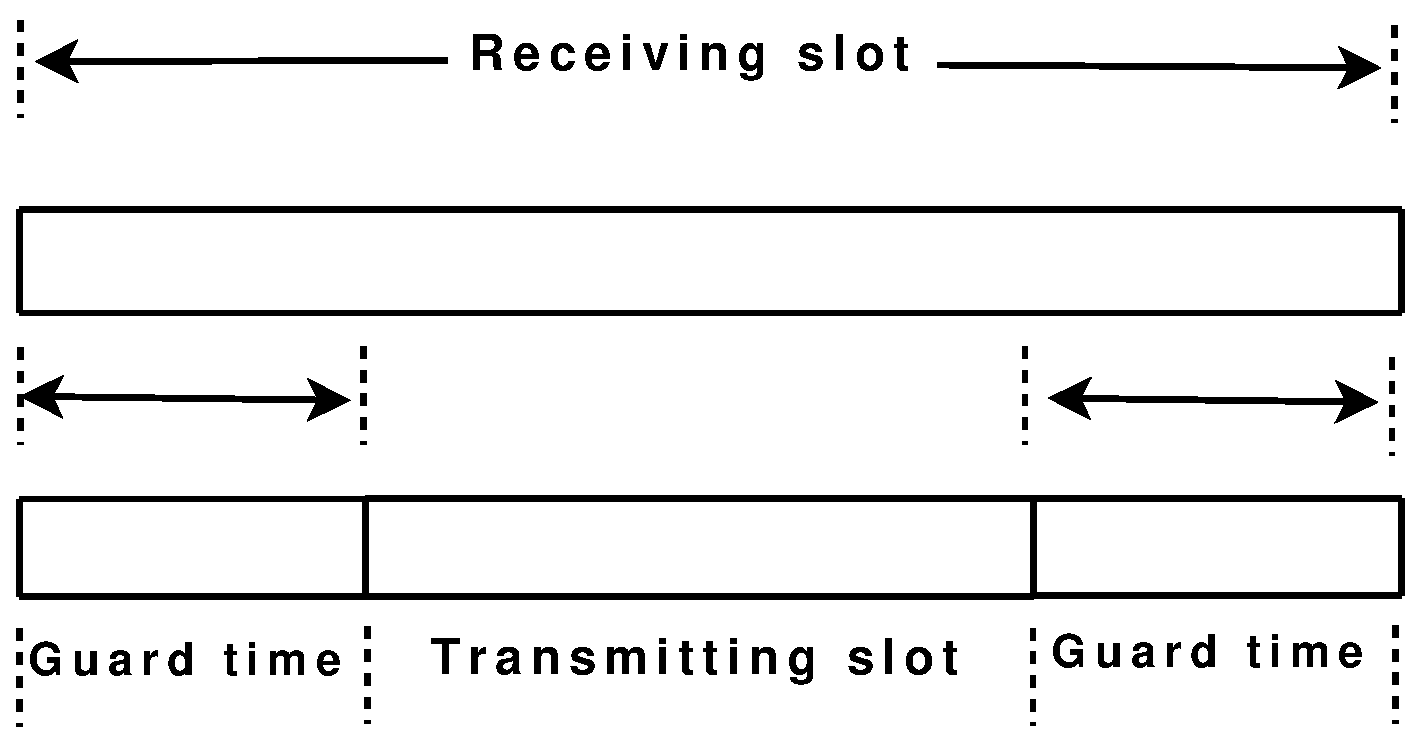
\includegraphics[width=0.6 \textwidth]{guardtime}
\caption{Guard time for drift compensation} \label{guardtime}
\end{figure}
\newline
A time slot can be defined as being expressed in a number of clock cycles as
\begin{equation}
t_{slot} = kT ,
\end{equation}
where $T$ is the period of the time frame in clock cycles and $t_{slot}$\nomenclature{$t_{slot}$}{Time duration of a slot} is the time duration of a TDMA slot and $k$ is the fraction.
\newline
With a synchronization period $T_{sync}$\nomenclature{$T_{sync}$}{Synchronization frequency} and the maximum clock drift of a clock $\rho$ , the maximum time difference between a sender and a receiver is
\begin{equation}
t_{diff} = 2\frac{T_{sync}}{T}\rho ,
\end{equation}
where the factor of $2$ reflects the worst case scenario where each node's clock drifts in the opposite direction.
\newline
Since the relative time difference between two nodes can be in two direction, the guard time, $t_{guard}$\nomenclature{$t_{guard}$}{Length of the guard time}, needs to be twice $t_{diff}$,
\begin{equation}
t_{guard}= 2t_{diff} = 4\frac{T_{sync}}{T}\rho.
\end{equation}
At this end, the minimum duration for a time slot $t_{slot}$ is
\begin{equation}
t_{slot} \geq t_{guard} + T_{tx},
\end{equation}
where $T_{tx}$ is a system constant and it represents the required time to send a packet from one node to other.
\newline Each message that is send within a time slot is exactly received by a neighbor at a known clock tick number
\begin{equation}
tick_{rx} = T_{tx}+ \frac{t_{guard}}{2} \label{tick}
\end{equation}
Hence, each time when a node receives a message, it has to be received exactly at the clock tick given by ($\ref{tick}$). Whenever
this number is not equal with the desired one, a phase error is observed.
\newline
Two nodes have a good communication link when they synchronize their clocks at least once every $T_{sync}$ that gives the following
relation,
\begin{equation}
\frac{T_{sync}}{T}\geq 1.
\end{equation}
It is a good practice to design systems having a $T_{sync}$ greater than the time frame. It increases the battery life of a node. However,
this has a negative impact on the communciation of the nodes.
\newline
To obtain the value of $T_{sync}$ for a particular system with a given duty cycle, we have to solve the next problem
\begin{equation}
t_{guard} \geq 4\rho \frac{T_{sync}}{T}
\end{equation}
\begin{equation}
t_{slot} \geq t_{guard} + T_{tx}
\end{equation}
\begin{equation}
\frac{T_{sync}}{T} \geq 1
\end{equation}
Hence, there is a trade-off in determining $T_{sync}$: increasing $T_{sync}$ reduces the energy costs of synchronization, but decreases the network perfromance. This is because the synchronization done less frequently so than nodes might drift out of synchronization in the mean time.
\section{\textbf{Lower bound of Synchronization}}
As in traditional distributed synchronization, a network of nodes equipped with hardware clocks with bounded drift is considered
here. Nodes compute logical clock values based on their hardware clocks and information that they have, and the goal is to
synchronize the nodes' logical clocks as closely as possible, while satisfying certain validity conditions. \newline
There are different approaches towards the lower bound that a synchronization algorithm achieve. In $\cite{gradient}$, the clock drift is taken to be zero and the delay impact on the lower bound of the synchronization algorithm is presented. But a more realistic approach is presented in $\cite{gradient2}$. Gradient clock synchronization is shown to require that the skew between any two nodes' logical clocks be
bounded by a nondecreasing function of the uncertainty in message delay (call this the distance) between the two nodes. Nearby nodes
are required to be closely synchronized, and allow faraway nodes to be more loosely synchronized. Hence, the result is that the worst
case clock skew between two nodes at distance $d$ from each other is
\begin{equation}
\Delta L \geq \frac{\tilde \rho d}{8(1+\tilde \rho)}\frac{log(n-1)}{log(\frac{8(1+\tilde \rho)}{\tilde \rho}log(n-1))}.
\end{equation}
where $n$ is the number of nodes in the network. This means that synchronization is not only a local property, in the sense that the clock skew between two nodes depends not only on the distance between the nodes, but also on the size of the network. \newline
Our lower bound implies, as in the case of MyriaNed, that the TDMA protocol with a fixed slot granularity will fail as the network grows, even if the maximum degree of each node stays constant.
\begin{figure}
\centering
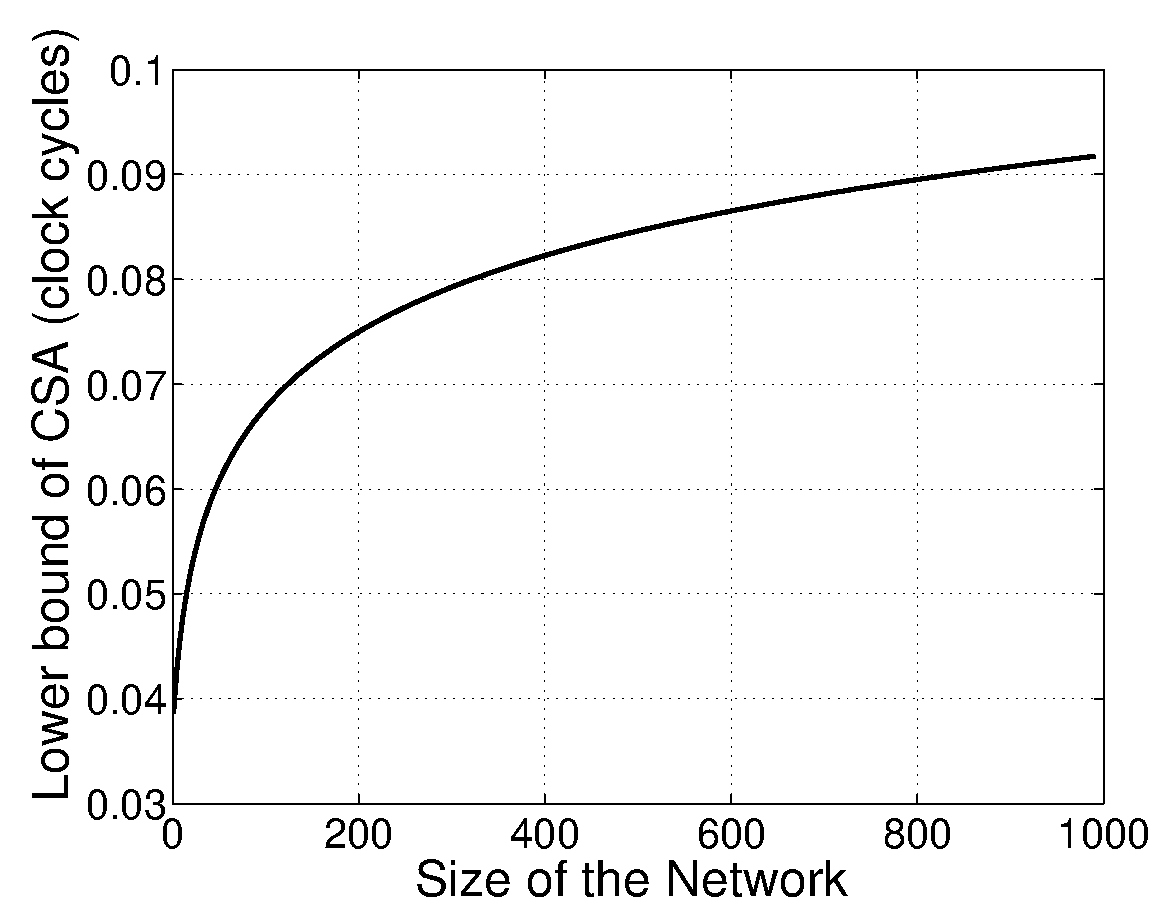
\includegraphics[width=0.5 \textwidth]{lowerbound}
\caption{Network size and the lower bound of Synchronization}
\label{gradient}
\end{figure}
As shown in Figure $\ref{gradient}$, as the network size grows, the lower bound of the synchronization also increases.
\section{\textbf{Mathematical Model}}
As it is described earlier, the wake up time of the nodes should be synchronized in such away that the nodes are synchronized in the
long term, as the TDMA scheduling requires. As part of the message, the nodes are transmitting the slot number which they are transmitting. This information is used in the calculation of the time that the message is sent.
\newline
The difference between the transmitting times of node $i$ and node $j$ is
\begin{equation}
\Delta t_{ij}^{(n)} = t_i^{(n)} - t_j^{(n)} ,
\end{equation}
where $t_i$ and $t_j$ are the wake-up times of node $i$ and node $j$ at the $n^{th}$ period. The wake-up time of a node at a random time
after $n$ periods of firings after it is turned on is
\begin{equation}
t_i^{(n)} = \sum_{n} T_i^{(n)} + t_{io},
\end{equation}
where  $T_i^{(n)}$ is the period of the crystal clock at the $n^{th}$ period since it changes with time according to
($\ref{frequency}$) and $t_{io}$ is the initial start-up time of the node. The frequency of the node varies due to the different factors
mentioned in ($\ref{frequency}$). \newline
The difference in the wake-up time of the nodes is given by
\begin{eqnarray}
\Delta t_{ij} & = & \sum_{n}T_i^{(n)} + t_{io}- (\sum_{n}T_j^{(n)} +
t_{jo}) \\ &=& (\sum_{n}T_i^{(n)} - \sum_{n}T_j^{(n)}) +
(t_{io}-t_{jo}).
\end{eqnarray}
The offset being applied should be able to compensate for the phase error introduced by the drift as well as the frequency changes. This
can be done using two approaches, which are not exclusive. The first one is adjusting the clock frequency to come up with a better
wake-up time. The second one is to adjust the next wake-up time depending on the difference between the current wake-up time of the
node and its neighbors. In this research, the second option is explored due to:
\begin{itemize}
\item The cost of adjusting the frequency of the clock: This is more expensive (hardware based) than adjusting the next wake-up time of the node.
\item The complexity of the implementation: The more complex the implementation is, the larger the energy consumption it will result in.
\end{itemize}
Application of offset compensating using prediction of the next wake up time is the promising approach to be implemented on the MyriaNode. The next wake-up time of the node is, thus, dependent on the current wake-up time of its neighbors in relation to its previous wake-up time,
\begin{equation}
t_i^{(n+1)} = t_i^{(n)} + T_i^{(n)} - \xi_i^{(n)} ,
\end{equation}
where $T_i$ is the period of the node's clock and $\xi_i$\nomenclature{$\xi_i$}{Offset to be added to Node $i$} is given by
\begin{equation}
\xi_i = f(\Delta t_{ij}).
\end{equation}
The function $f$ is based on an algorithm which takes the wake-up time differences between the node and its neighbors and determines
the optimal offset to be added to the next wake-up time of the node.
\newline Different algorithms are presented here and discussed with the simulation results presented in the next chapter of the report.
\subsection{\textbf{Weighted Measurements - Interference-phobic approach}}
One form of approach to tackle the dynamic behavior of a wireless sensor network, due to channel conditions as well as collisions, is a
Weighted Measurement (WM\nomenclature{WM}{Weighted Measurements}) approach. Using this approach, different weight is given to the different phase error measurements. A weight is added to the increase the influence of the close by neighbors and ensure faster synchronization. In addition to that, a new joining neighbor can get synchronized with out disturbing the existing neighbors, adjusting its time to the big swarm of nodes. Its a metaphor of "The Majority Wins". Hence,
\begin{equation}
\xi_i^{(n)} = \sum{w_{ij}^{(n)}\Delta t_{ij}^{(n)}} ,
\end{equation}
where $\sum{w_{ij}^{(n)}= 1}$.
\newline
The weighted adjustment is used to modify the local wake-up time of the node,
\begin{eqnarray*}
t_i^{(n+1)} &=& t_i^{(n)} + T_i^{(n)} - \xi_i^{(n)} \\ &=& t_i^{(n)}
+ T_i^{(n)} - \sum_{j=0}^N{w_{ij}^{(n)}\Delta t_{ij}^{(n)}} \\ &=&
t_i^{(n)}+ T_i^{(n)} -
\sum_{j=0}^N{w_{ij}^{(n)}(t_i^{(n)}-t_j^{(n)})} \\ &=& T_i^{(n)} + \sum_{j=0}^N{w_{ij}^{(n)}t_j^{(n)}}.
\end{eqnarray*}
\newline
The main task in this algorithm is how to choose the weight factors so that the stability of the network (timewise) is achieved in a faster time. In order to see how the weight factors should affect the next wake-uptime of the node, we will discuss scenarios.
\newline
The weight is selected by the fact that the a node joining a network should adjust its time with the network that it is joining. After
each measurement, a phase error is associated with the tabled values to recognize how far is the sending node concerning the time that it
drifted away from the receiving node. The weights are calculated as:
\begin{equation}
\delta_{ij} = ae^{-b\Delta t_{ij}}.
\end{equation}
The parameters are selected using the initial conditions, $\delta_{ij}=0.1$ for $\Delta t_{ij}$ = $t_{guard}$ and $\delta_{ij}=1$ for $\Delta t_{ij}$ = 0.
\newline
As shown in Figure $\ref{weight}$, the closer the phase error is to zero, the higher weight it is given. The assignment of high
values to the small phase errors will decrease the time it takes to synchronize this node with the network.
\begin{figure}
\centering
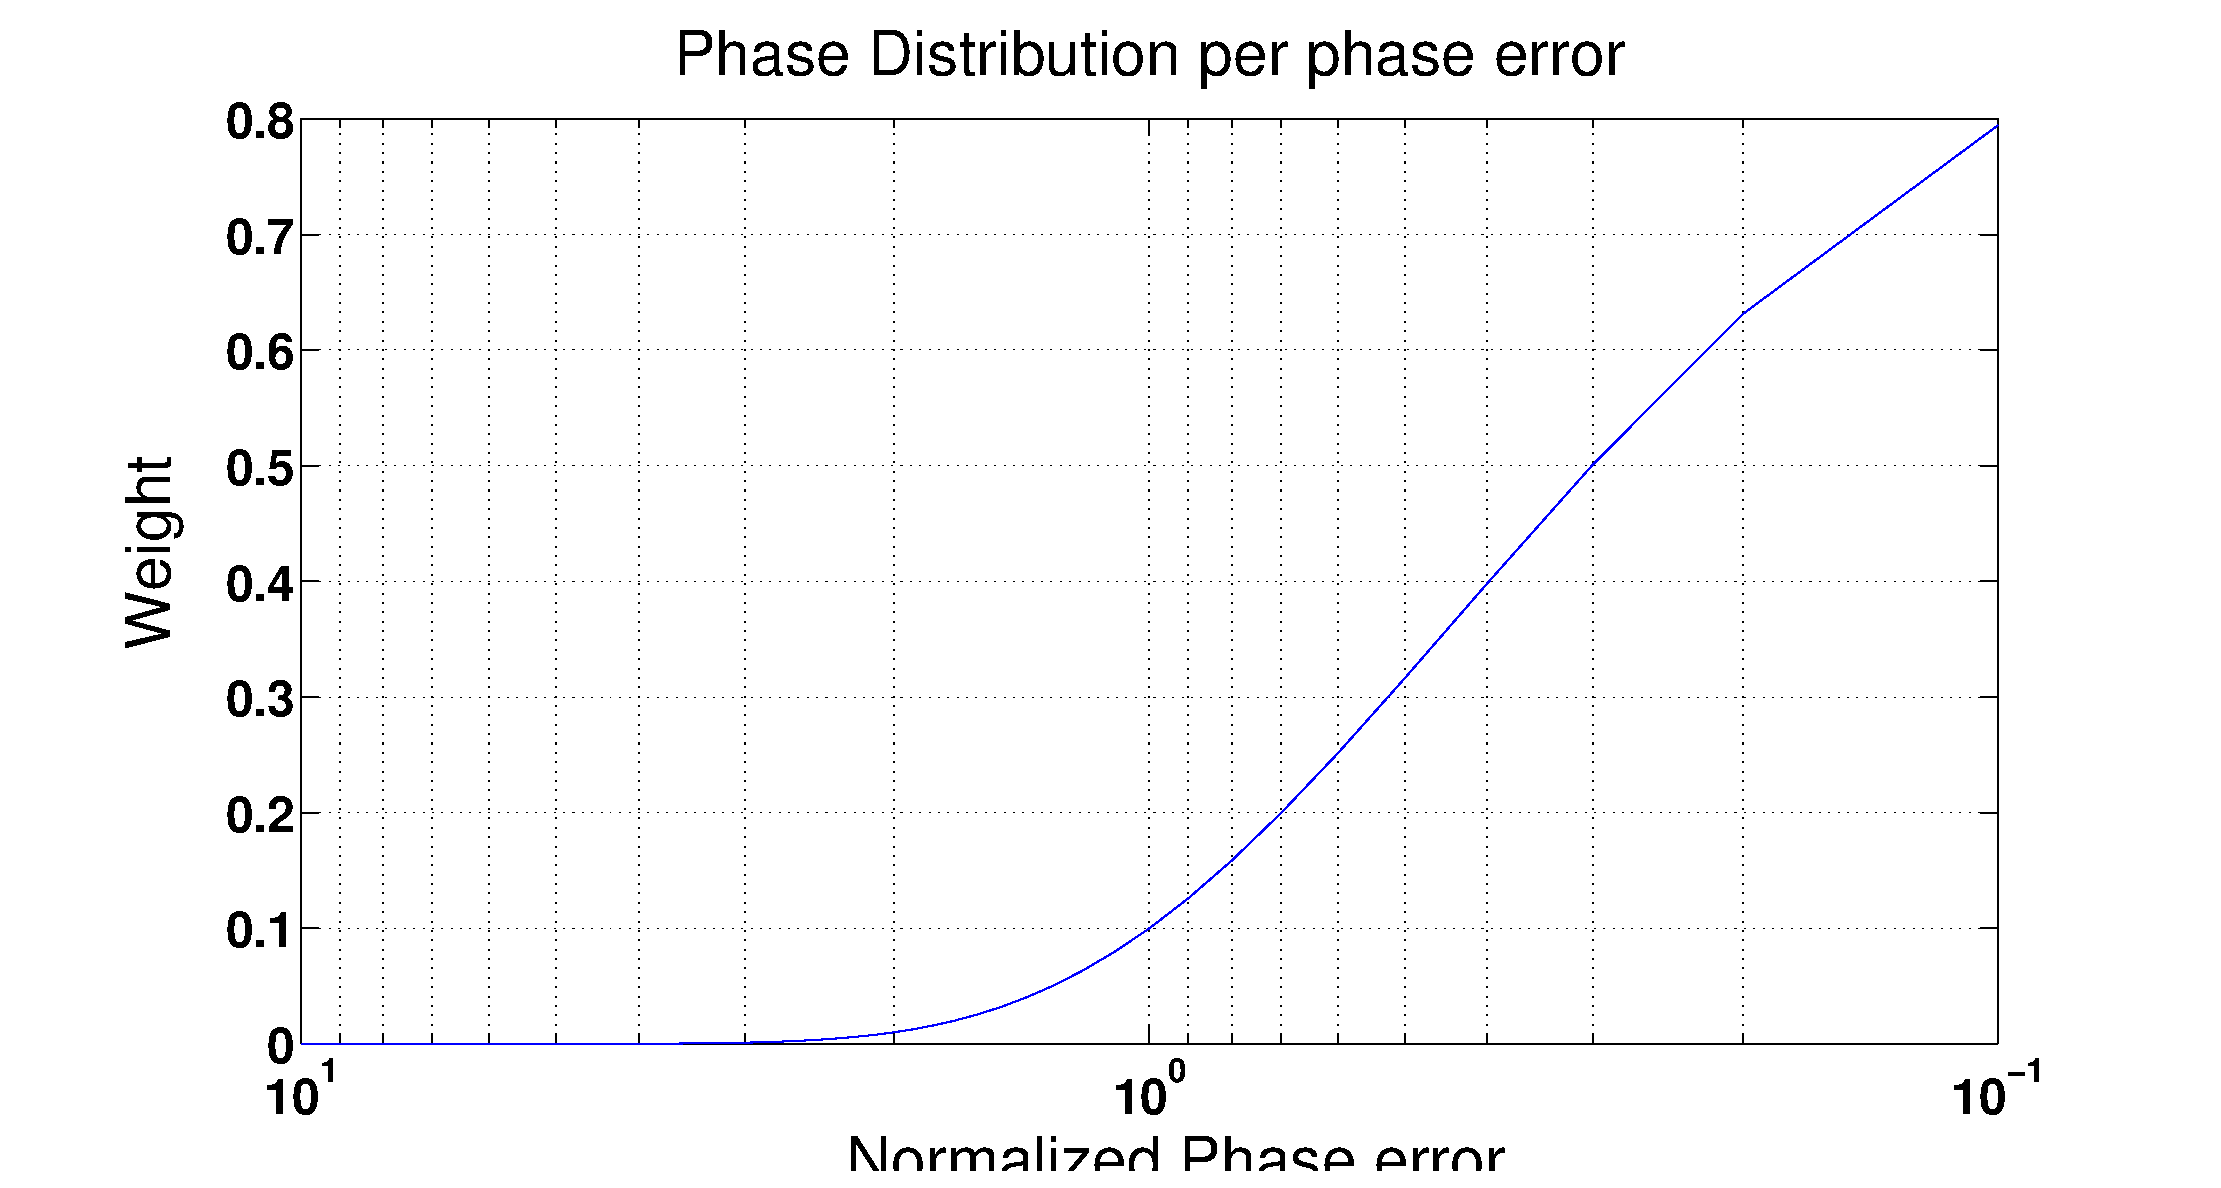
\includegraphics[width= 0.6 \textwidth]{weight}
\caption{Weight factors for the phase error distribution}
\label{weight}
\end{figure}
\newline
In the assignment of the weight factor, there is another issue to be considered. If all the phase errors are in the lower region, this
corresponds to the fact that the node is a newly joining node to a well-established and synchronized network.  In order to incorporate the
effect of the distribution of the phase errors, another quantity, $\delta$, is introduced in the calculation of the weight factors so
that the node will adjust its wake-up time towards the more stabilized network. This parameter expresses the distribution of the
weight factors,
\[w_{ij} = \left\{
\begin{array}{l l}
  1 - \delta_{ij},& \quad \mbox{if $m(\delta_{ij}$) $<$ 0.5}\\
 \delta_{ij}, & \quad \mbox{if $m(\delta_{ij}$) $>$ 0.5}\\ \end{array} \right. \]
 where $m$ is the mean function.
\newline
Hence, the weight moves towards the large phase errors if the node is a new-comer which wants to join the "already established" network. WM is a two step process in which the first one describes how the nodes is offsetted from its neighbor whereas the second one describes how the node is positioned in the network topology which surrounds it.
\newline
Using the weighted approach, a series of measurements will be used to estimate the next wake-up time of the node, giving less
value/emphasis to the nodes which are out of reach from the other nodes. The simulation result is shown in the next section to see the
effect of the algorithm in comparison to the other algorithms.\newline \newline
\begin{tabular}{  l }Algorithm for WM \\\hline \hline
1. Nodes broadcast packets. \\  2. Each receiver records the time that the packet is received. \\
3. Each receiver i computes its phase error to any other node j in the neighborhood. \\
4. Each receiver i computes the weight factor for the corresponding phase error. \\
5. Each receiver i computes the offset using the weigh factor method. \\
6. Each receiver adjusts its wake up time using the offset.\\
\hline \hline
\end{tabular}
\subsection{\textbf{Non Linear Least Squares method}}
\subsubsection{Non Linear Least Squares}
In this section, another approach is used for synchronization of the nodes.
\newline
\begin{figure}
\centering
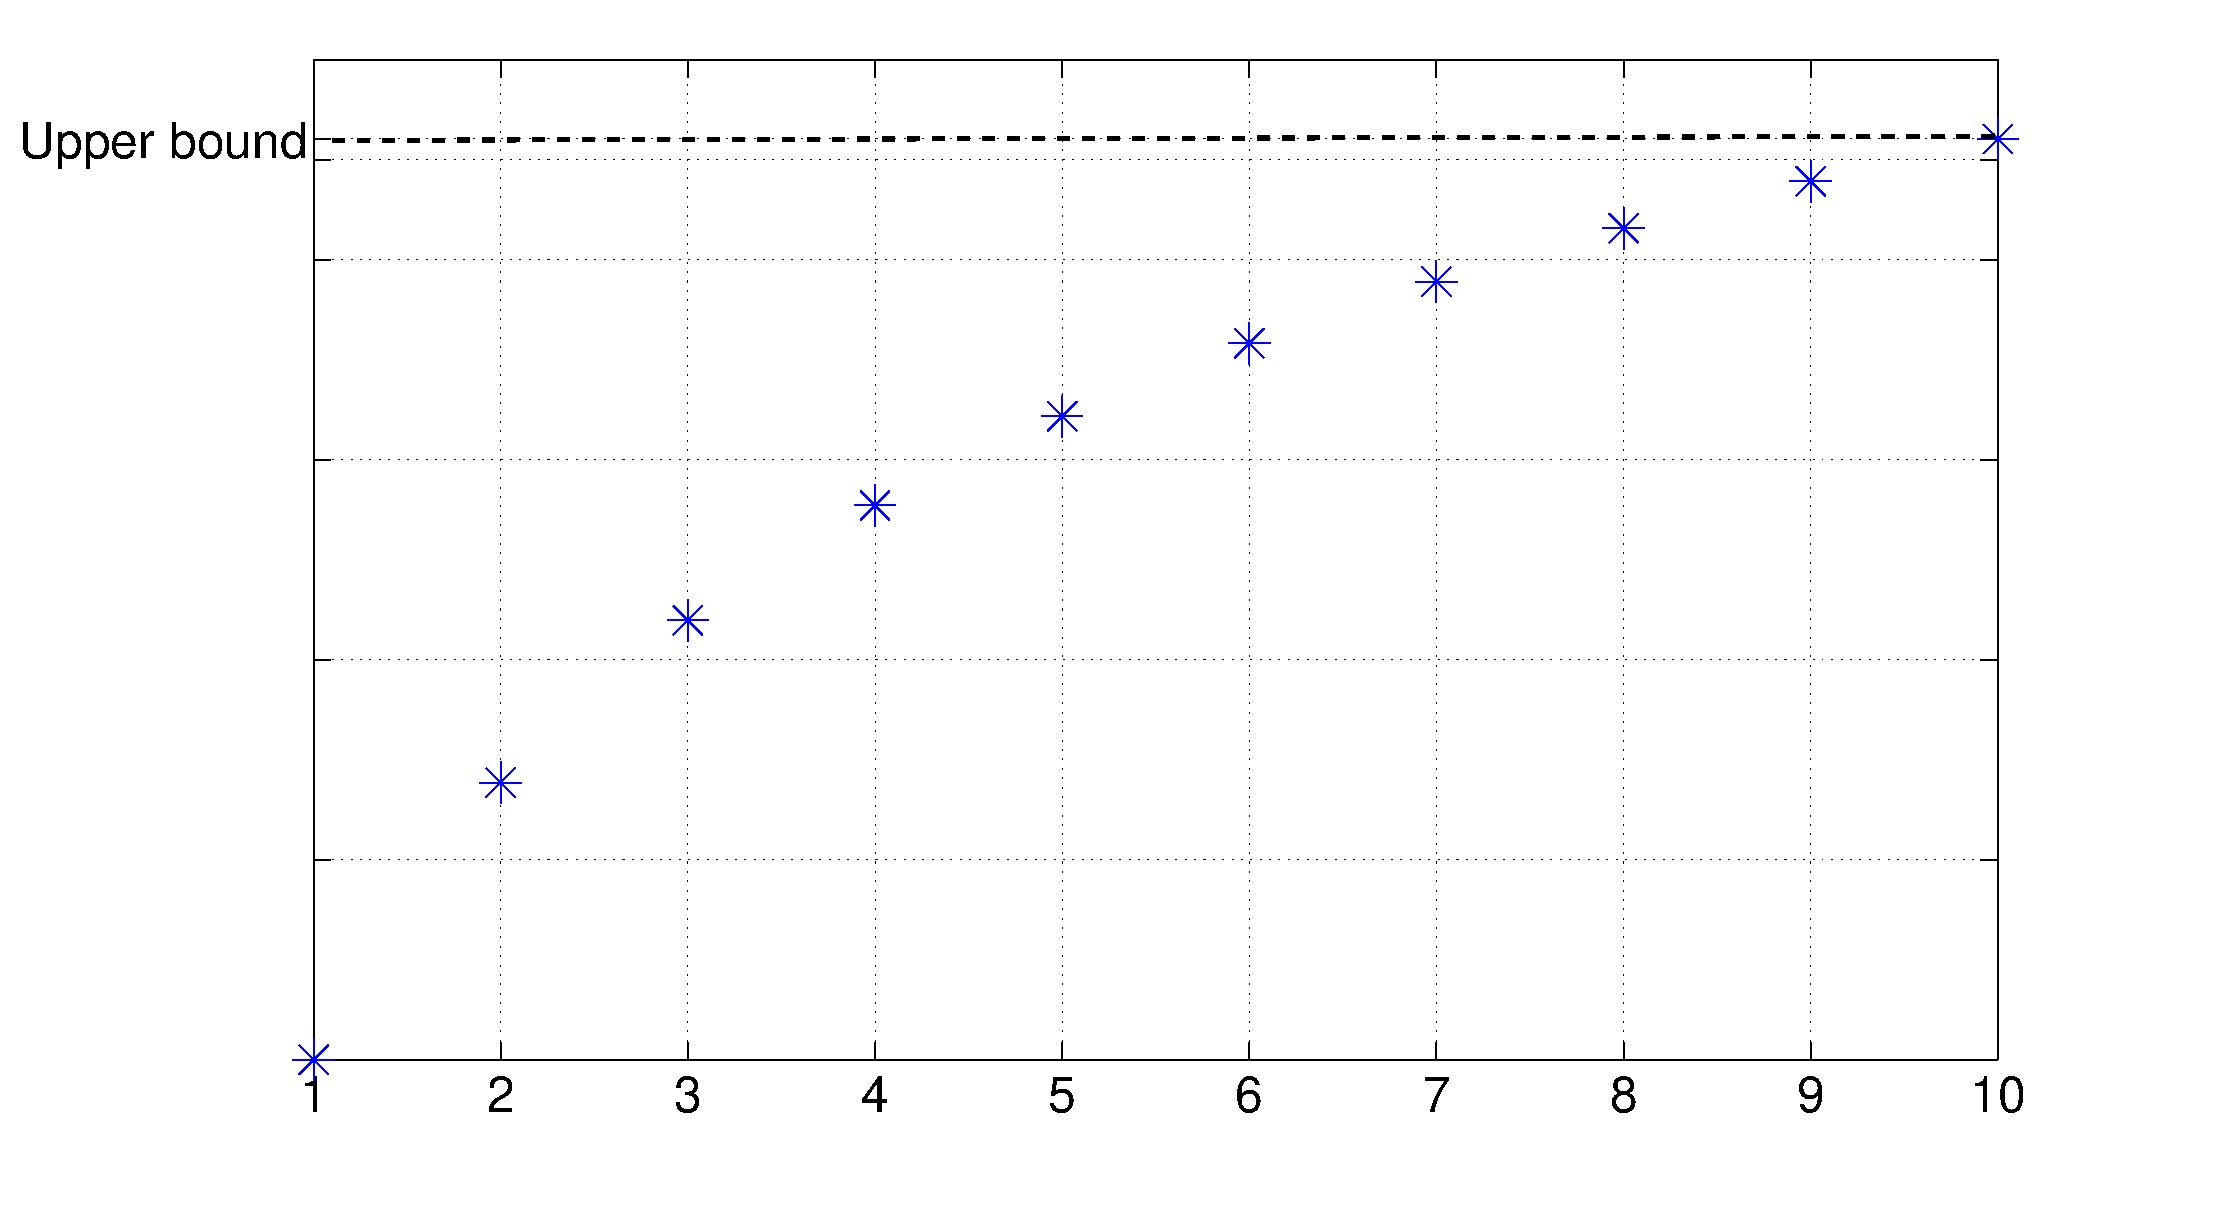
\includegraphics[width=0.75 \textwidth]{curvefit}
\caption{Curve fitting using logarithmic function} \label{curvefit}
\end{figure}
Normalized phase error values tend to be small and follow a curve in such away that the maximum value of the phase error should not be greater than the threshold value that was intended to be. See Figure $\ref{curvefit}$.
\newline
Non Linear Least Squares (NLLS\nomenclature{NLLS}{Non Linear Least Squares}) Curve Fitting  is a mathematical procedure for finding the best fitting curve to a given set of points by minimizing the sum of the squares of the offsets ("the residuals") of the points from the curve. In order to fit the curve, we have chosen the logarithmic curve in order to meet the demand of adjusting the time offset and stabilize the network. A logarithmic function can be used to represent the distribution of the offsets in the neighborhood,
\begin{equation}
 f(x_i,\beta)= \beta _1 + \beta_2 log(x_i),
\end{equation}
where $\beta_1$ and $beta_2$ are the parameters to be estimated.\newline
A set of $n$ data points(corresponding to $n$ neighbors) which are ($x_1$, $y_1$), ($x_2$, $y_2$),$\dots$,($x_n$, $y_n$), and a curve (model function) $y= f(x, \beta)$, that in addition to the variable $x$ can be used to estimate the next wake-up time of the node.
\newline
It is desired to find the vector $\beta$ of parameters,$\beta_1$ and $\beta_2$, such that the curve fits best the given data in the least squares sense, that is, the sum of squares
\begin{equation}
    S=\sum_{i=1}^{m}r_i^2 ,
\end{equation}
is minimized, where the residuals $r_i$ are given by
\begin{equation}
    r_i = y_i - f(x_i,\beta)
\end{equation}
for i=1,2,$\dots$, $n$.
\newline
The minimum value of $S$ occurs when the gradient is zero. There are gradient equations to be solved:
\begin{equation}
    \frac{\partial S}{\partial \beta_j}=2\sum_i r_i\frac{\partial r_i}{\partial \beta_j}=0 \ (j=1,2).
\end{equation}
In a non-linear system, the derivatives $\frac{\partial r_i}{\partial \beta_j}$ are functions of both the independent variable and the parameters. These gradient equations do not have a closed solution. Instead, initial values must be chosen for the parameters. Then, the parameters are refined iteratively, that is, the values are obtained by successive approximation,
\begin{equation}
    \beta_j^{k+1}=\beta^k_j+\Delta \beta_j.
\end{equation}
Here, $k$ is an iteration number and the vector of increments, $\Delta \beta_j$, is known as the shift vector. At each iteration,
the model is linearized by approximation to a first-order Taylor series expansion about $\beta^k$.
\begin{equation}
    f(x_i,\beta)\approx f(x_i,\beta^k) +\sum_j \frac{\partial f(x_i, \beta^k)}{\partial \beta_j} \left(\beta^k_j -\beta_j \right)
\end{equation}
\begin{equation}
 f(x_i,\beta) =f(x_i, \beta^k)+\sum_j J_{ij} \Delta\beta_j.
\end{equation}
The Jacobian, $J$, is a function of constants, the independent variable and the parameters, so it changes from one iteration to the
next. Thus, in terms of the linearized model,
\begin{equation}
\frac{\partial r_i}{\partial \beta_j}=-J_{ij}
\end{equation}
and the residuals are given by
\begin{equation}
    r_i=\Delta y_i- \sum_{j=1}^{j=n} J_{ij}\Delta\beta_j,
\end{equation}
where
\begin{equation}
 \Delta y_i=y_i- f(x_i, \beta^k).
\end{equation}
Substituting these expressions into the gradient equations and equating to $0$, we get a matrix notation of
\begin{equation}
    \left(J^TJ\right)\Delta  \beta=J^T\Delta y
\end{equation}
When the observations are not equally reliable, as in case of WSNs which are being studied, a weighted sum of squares may be minimized
using the weights( Figure $\ref{weight}$ ),
\begin{equation}
    S=\sum_{i=1}^{i=m}W_{ii}r_i^2.
\end{equation}
The normal equations are then
\begin{equation}
    \left(J^TWJ\right)\Delta  \beta=J^TW\Delta y.
\end{equation}
\subsubsection{Model Design}
As the algorithm is decentralized, the next wake-up time of the node depends on the current offset that it has with the other nodes. The distribution of the offset is the crucial factor in deciding the type of curve which we want to fit in. The phase error shows how many time units that the neighbor node is out of touch with the node in focus. The larger the phase error is, the more out-of-sync the node is. This happens because of
\begin{itemize}
\item nodes joining the network
\item interference from the environment
\item clock drift
\item mobility of Nodes
\end{itemize}
Since these nodes might have been long enough without synchronizing, the phase error that they are going to have is large compared to the
nodes which were in the neighborhood during the last round of communication. Thus, to join the mass of the network rather than the
mass joining the single node, the algorithm is required to push the synchronization towards the more established network, rather than
away.\newline
The set of data are the measured phase error of the node and the parameters $\beta_1$ and $\beta_2$ are estimated using a least
squares approximation.
\begin{equation}
 f(x_i,\beta)= \beta _1 + \beta_2log(x_i),
\end{equation}
The initial values of the parameters $\beta_1$ and $\beta_2$ is estimated taking into account the state of the network to be. Hence, for the perfect function of log estimation.
i.e. \newline \newline
As each measurement arrives from the neighbors, an iteration is made in such a way that the measurement error from a pre-determined offset value is reduced. This ensures that the offset to be added in the next wake-up time doesn't diverge in a large amount from the predicted value. Hence, the difference in measured values and thus the offset is considered big. In the desire to stay in the originally stabilized
network, the nodes tendency to adapt a new environment is very low, in this case resisting any change that is going to happen to its
wake-up time. \newline
\newline
\begin{tabular}{  l }Algorithm for NLLS \\\hline \hline
1. Nodes broadcast packets. \\  2. Each receiver records the time that the packet is received. \\
3. Each receiver i computes its phase error to any other node j in the neighborhood. \\
4. Each receiver i computes the optimal curve fit for the corresponding phase errors. \\
5. Each receiver i computes the offset using the function. \\
6. Each receiver adjusts its wake up time using the offset.\\
\hline \hline
\end{tabular}
\subsection{\textbf{Discrete time Kalman Filter for synchronization}}
\subsubsection{Discrete time Kalman Filter}
The Kalman filter estimates a process by using a form of feedback control: the filter estimates the process state at some time and
then obtains feedback in the form of (noisy) measurements. As such, the equations for the Kalman filter fall into two groups: time
update equations and measurement update equations. The time update equations are responsible for projecting forward (in time) the
current state and error covariance estimates to obtain the a priori estimates for the next time step.
\newline
The Kalman filter addresses the general problem of trying to estimate the state $x$ of a discrete-time controlled process that is
governed by the stochastic difference equation
\begin{equation}
 x_k = Hx_{k-1} + Bu_k + w_{k-1} ,
\end{equation}
with a measurement $z$ that is
\begin{equation}
 z_k = Hx_k + v_k.
\end{equation}
The random variables $w_k$ and $v_k$ represent the process and measurement noise ( respectively). They are assumed to be independent( of each other), white, and with normal probability distributions
\begin{equation}
 p(w) \approx N(0,Q),
\end{equation}
\begin{equation}
 p(v) \approx N(0,R).
\end{equation}
With the initial estimates of $x_{k-1}$ and $P_{k-1}$
\begin{equation}
x_k = Hx_{k-1} + Bu_k
\end{equation}
\begin{equation}
P_k = HP_{k-1}H^T + Q
\end{equation}
The measurement update equations are responsible for the feedbacks i.e. for incorporating a new measurement into the a priori estimate
to obtain an improved a posteriori estimate.
\begin{equation}
K_k = P_kH^T(HP_kH^T + R)^{-1} \label{kalmangain}
\end{equation}
\begin{equation}
x_k = x_k + K_k(z_k - Hx_x)
\end{equation}
\begin{equation}
P_k = (I-K_kH)P_k
\end{equation}
The time update equations can also be thought of as predictor equations, while the measurement update equations can be thought of as corrector equations.
\newline
Hence, a priori and a posteriori estimate errors are defined as
\begin{equation}
e_k^- = x_k – \tilde x_k^- ,
\end{equation}
\begin{equation}
e_k =  x_k – \tilde x_k.
\end{equation}
The a priori estimate error covariance is then
\begin{equation}
P_k^- = E[ e_k^- e_k^{-T} ]
\end{equation}
and the a posteriori estimate error covariance is
\begin{equation}
P_k = E[e_k e_k^T]
\end{equation}
Following these, we can see the equation more deeply.
\begin{equation}
\tilde x_k = \tilde x_k + K(z_k-H\tilde x_k).
\label{updatekalman}
\end{equation}
The difference $z_k - H\tilde x_k$ in $\ref{updatekalman}$ is called the the residual. The residual reflects the discrepancy between the
predicted measurement $H\tilde x_k$ and the actual measurement $z_k$. A residual of zero means that the two are in complete
agreement. \newline
The matrix K in ($\ref{kalmangain}$) is chosen to be the gain or blending factor that minimizes the posteriori error covariance. Taking the derivative of the trace of the result with respect to K, setting that result equal to zero, and then solving for K, we get
\begin{equation}
K_k = P_kH^{T}(HP_kH^{T} + R)^{-1}
\end{equation}
\begin{equation}
K_k = \frac{P_kH^T}{HP_kH^T + R}.
\label{gain}
\end{equation}
Looking at ($\ref{gain}$), it is seen that as the measurement error covariance $R$ approaches zero, the gain K weights the residual more
heavily. Specifically,
\begin{equation}
\mathop {\lim }\limits_{R_k \to 0 } {K_k} = H^{-1}.
\end{equation}
On the other hand, as the a priori estimate error covariance $P_k$ approaches zero, the gain K weights the residual less heavily. Specifically,
\begin{equation}
\mathop {\lim }\limits_{P_k \to 0 } {K_k} = 0.
\end{equation}
\subsubsection{Model design}
In the selection of the matrices for the synchronization algorithm, we will consider different situations of the WSN.
\newline
The transition matrix $H$ plays an important role in achieving the proper synchronization as it determines the weight that should
be put in the previous value. It indicates how fast/slow is the next wake up time should be compared to it's previous value and/or neighbors. With the stable network where the nodes remain intact, the wake-up time of the node is expected to be the same despite the clock drift.
\newline
The initial estimates are selected from the previous firing time of the node. Hence,the initial values of $x$ and $P$ are estimated from the previous values, one period earlier. This ensures that the nodes are on the same track as the previous time, since the neighbors remain the same with some exception of mobility and interference. \newline
Hence, to tackle the dynamic nature of the WSN, the new node joining the network should be synchronized with the already established "status quo" of the network. In the filter design, the covariance matrices $R$ and $Q$ also have a significant role in the overall implementation of the algorithm. $R$ represents how we value the measured values to affect the result of the outcome and $Q$ sends a signal as to how we have to evaluate the estimated value. \newline The estimated values, which base on a stable background are more prone to be right after a series of firings. On the contrary, the measured values have large deviations in such away that more of the weight is going to the estimated values, tending to stabilize the network. \newline The update equations are applied in the series of measurement
to end up in an optimal(next time) wake-up time of the node.
\newline  \newline
\begin{tabular}{  l }Algorithm for Kalman Filter \\ \hline \hline
1. Nodes broadcast packets. \\  2. Each receiver records the time that the packet is received. \\
3. Each receiver i computes its phase error to any other node j in the neighborhood. \\
4. Each receiver i computes the optimum Kalman update value for the phase errors. \\
5. Each receiver adjusts its wake up time using the offset calculated.\\
\hline \hline
\end{tabular}
\section{\textbf{Reducing the guard time}}
As the performance of the algorithms increases, the guard time can also be reduced to conserve energy. This inturn
reduces the duty cycle.
\begin{figure}
\centering
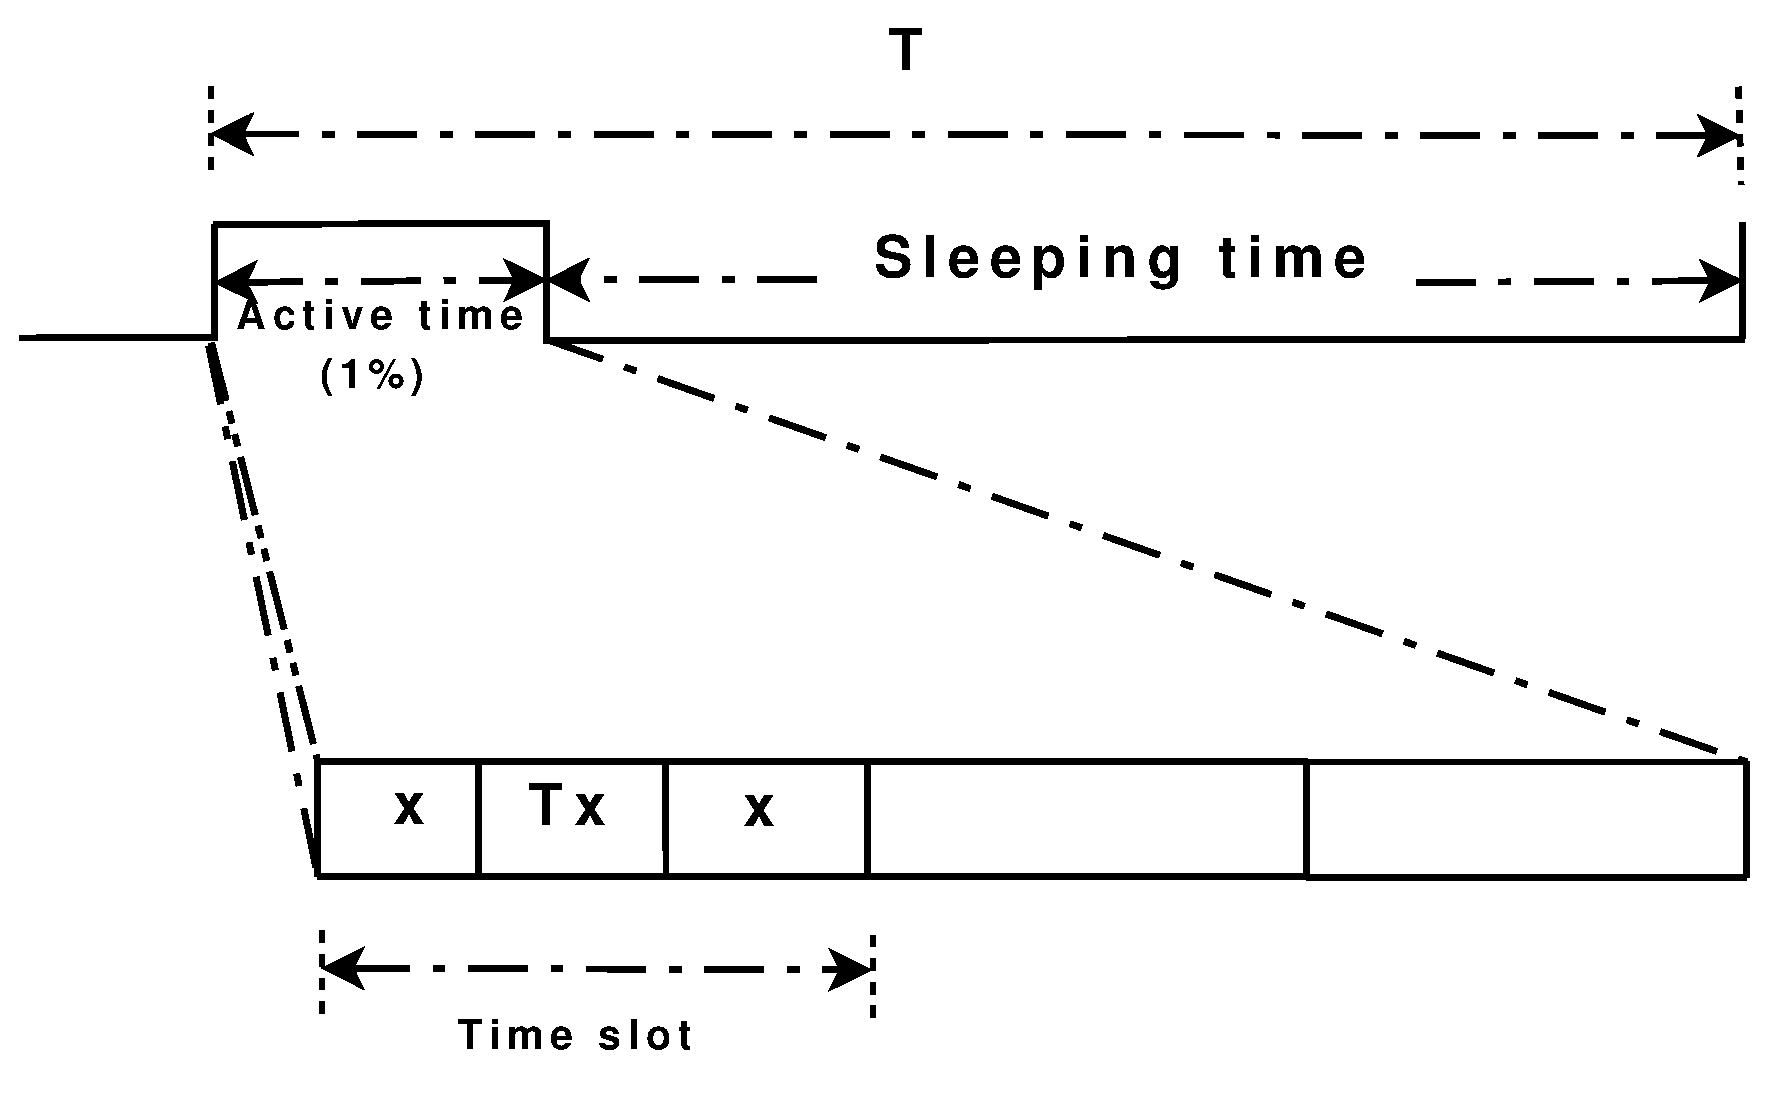
\includegraphics[width=0.6\textwidth]{guardtimesaving}
\caption{Guard time and } \label{guardtimesaving}
\end{figure}
\newline
Let $x$ denote the guard time when the median algorithm is implemented (Figure $\ref{guardtimesaving}$). Thus, the slot
duration will be
\begin{equation}
T_{slot}=2x + T_x ,
\label{slot}
\end{equation}
where $T_x$ is the transmit time of the node.
\newline
With $N$ slots, the duty cycle is then
\begin{equation}
D = \frac{NT_{slot}}{T}, \label{duty}
\end{equation}
where $T$ is the period of a time frame. \newline Substituting ($\ref{slot}$) in ($\ref{duty}$) equation, the duty cycle becomes
\begin{equation}
D= \frac{N(2x+T_{slot}}{T}.
\end{equation}
With the better performance achievement with the other algorithms, the guard time can be reduced depending on the precision of the
algorithm. Let $\epsilon$ be the guard time reduction in clock cycles. Hence, the new guard time will be $2x-\epsilon$.
\newline The new duty cycle becomes
\begin{equation}
D_n=\frac{(2(x-\epsilon)+T_x)N}{T}.
\end{equation}
Arranging the equation results in
\begin{equation}
D_n= \frac{(2x+T_x)N}{T} - \frac{(2\epsilon)N}{T}.
\end{equation}
Hence, with a performance increase in $\epsilon$ clk results in the duty cycle reduction of
\begin{equation}
D - D_n = \frac{(2\epsilon)N}{T}.
\end{equation}
The decrease in the guard time of the slot is thus dependent on the algorithm's performance ($\epsilon$) and the number of slots in the
frame. As the number of slots increases with a constant performance increase $\epsilon$, the energy conservation also increases linearly. The number of slots is determined by the MAC protocol.
\chapter{\textbf{Results and Discussion}}
\section{\textbf{Simulation setup}}
The simulation setup which is used in the research to test the performance of the presented frame synchronization algorithms is explained in this section. The simulated WSN operates in the 2.4GHz ISM band at a data rate of 2Mbps. We use a Discrete Event Simulator (DES) for the simulation.
\newline
A DES\nomenclature{DES}{Discrete Event Simulator} will break down a simulation into discrete chunks. Every event will occur at some countable time moment and will be given in chronological order. The advantage of this distinction is two-fold. First, simulations will not be dependant on some real-time clock, which reduces the inaccuracies fed into the simulation. Second, events can be isolated to perform certain measurements.
\newline
One such DES is called OMNeT++$\cite{omnet}$. It provides a component architecture for models. Components are programmed in C++, then assembled into larger components and models using a high-level language. These components are merged into a joined simulation environment: MiXiM$\footnote{MiXiM (MIXed sIMulator) is a simulation framework for wireless and mobile networks using the OMNeT++ simulation engine.It is a collaborative project  between TU Berlin, TU Delft and Universitaet Paderborn.}$.\newline
Nodes are modeled as a set of separate components stacked upon each other. Octave$\footnote{Octave is a free program for performing numerical computations which is mostly compatible with MATLAB. It is part of the GNU project.}$ is used for
interpretation of the data from the network simulator.
\newline
\begin{figure}
\centering
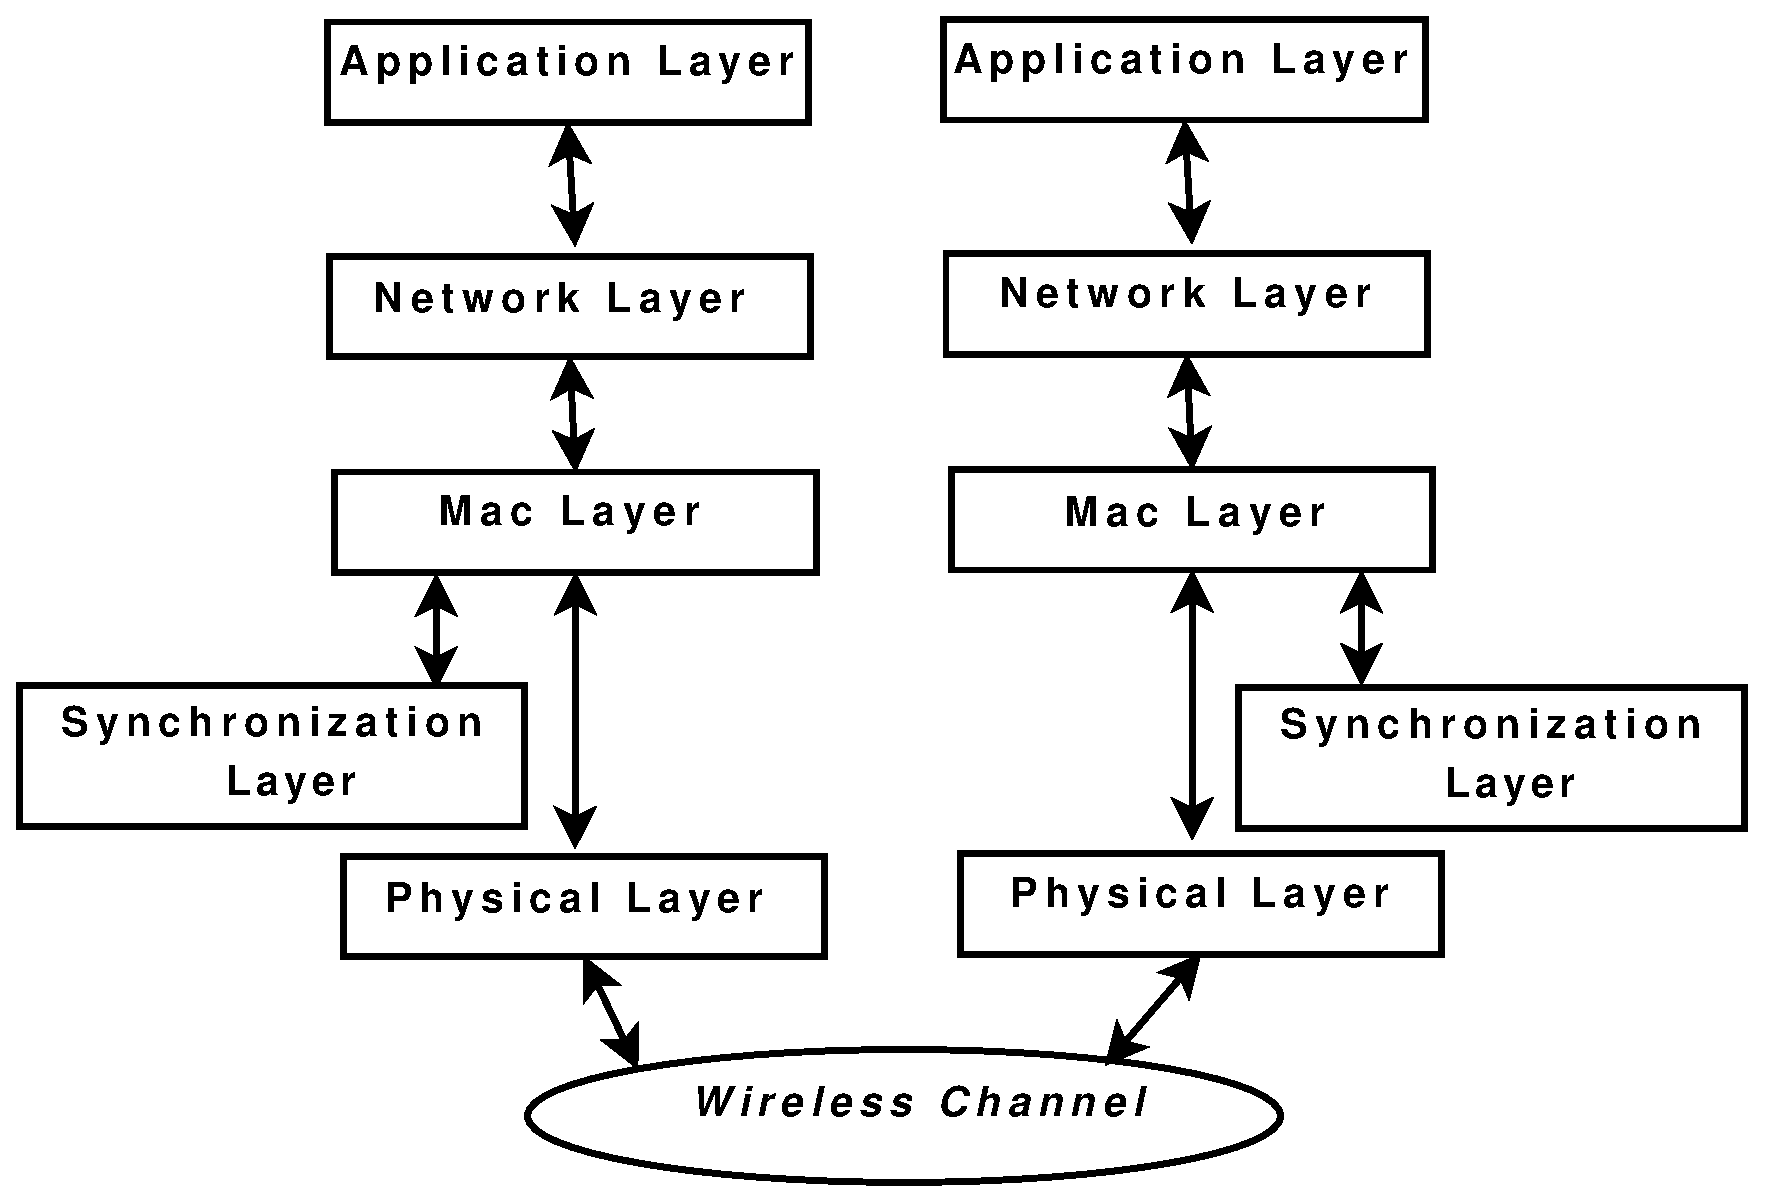
\includegraphics[width=0.6\textwidth]{osimodel}
\caption{Abstraction Model} \label{osimodel}
\end{figure}
As shown in Figure $\ref{osimodel}$, the synchronization is computed in a separate abstaraction layer. Each time the message is received, the time of arrival is recorded and used to calculate the next wake up time of the node. The communication over the channels is done in a unidisc way. All nodes in range of the radio receive the data, and those that are outside are excluded.
\newline
The number of nodes is varied for different scenarios. The movement of the nodes is modeled from the static to an average speed of a slowly moving object. The simulation is conducted 1000 times to counter the effect of randomness introduced in the simulation.
\section{\textbf{Simulation Results}}
The nodes are deployed uniformly across the field. The neighborhood is limited to 10 nodes. The start up time of the nodes is random, Gaussian distributed variable, $t_{io}$. The synchronization error is the maximum difference between the wake-up time of the nodes in the neighborhood.
\newline
\begin{center}
    \begin{tabular}{ | l | l |}
    \hline
    Duration time frame & 1s \\ \hline
    Radio range & 10 - 30m \\ \hline
    \end{tabular}
\end{center}
\subsubsection{\textbf{Case I}}
\begin{figure}[!h]
\centering
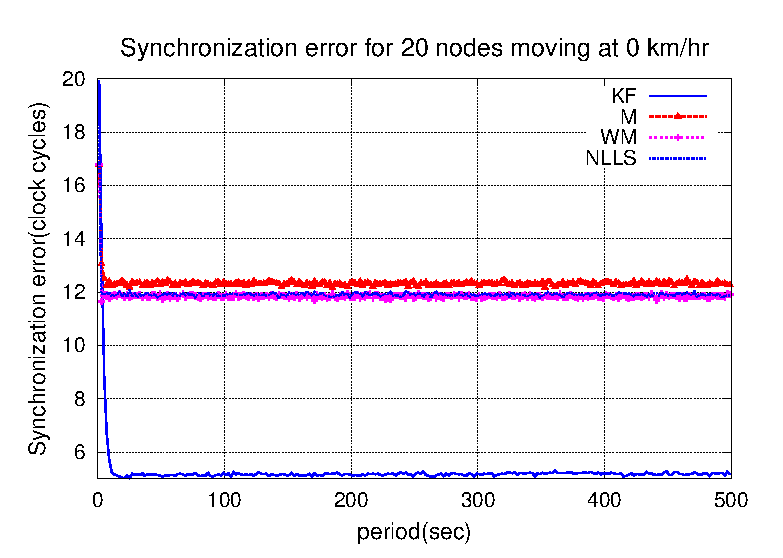
\includegraphics[width=0.7\textwidth]{16output-s0}
\caption{Synchronization error for 20 nodes - Static} \label{16output0}
\end{figure}
In the first set of simulation, the synchronization error is simulated for the nodes which are static,hence no effect of mobility. The number of nodes is taken to be $20$ and $50$ in the set of simulations.  \newline
\begin{figure}
\centering
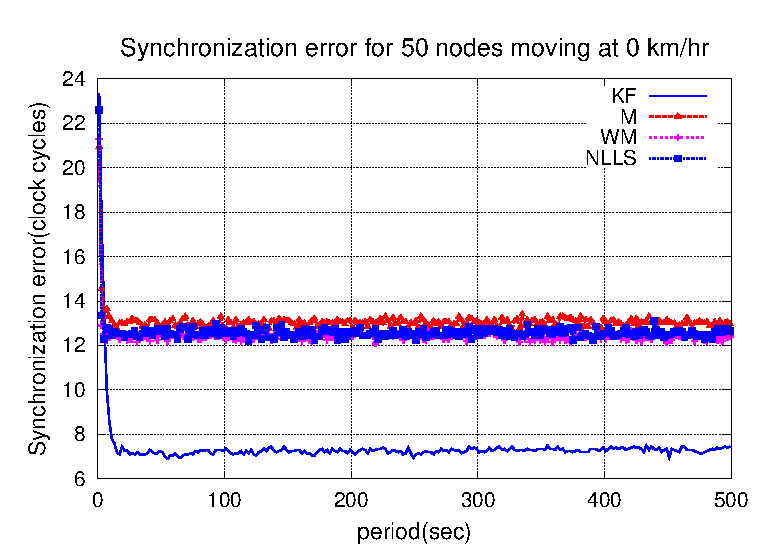
\includegraphics[width=0.7\textwidth]{50output-s0}
\caption{Synchronization error for 50 nodes - Static} \label{50output0}
\end{figure}
Figure $\ref{16output0}$ shows the synchronization error for $20$ nodes operating in a static environment. KF\nomenclature{KF}{Kalman Filter} has the lowest precision of synchronization error, at an avergage of $4clk$. NLLS and WM perform similarly at average precision of $12clk$ while Median performs well at $13clk$. \newline
Figure $\ref{50output0}$ is the result of a simulation for $50$ nodes. The synchronization error in general increases as the number of nodes increases the number of neighbors. Comparing the individual algorithms, KF has over $7clk$ performance improvement than the Median whereas NLLS and WM have a better performance ($1clk$) than the Median.
\subsubsection{\textbf{Case II}}
In second set of simulations, the mobility of the nodes is taken into account. Here, the number of the nodes is taken to be $20$. The simulations are conducted for different speeds, at $6km/hr$ and $20km/hr$. Chosen speeds emulate the speed of a walking man and an average speed of a slowly moving vehicle.
\newline
Figure $\ref{16output6}$ shows 20 nodes with a an speed which is an independent gaussian variable with mean $6km/hr$ and standard deviation of 1$km/hr$. As the results shows, WM and NLLS perform better the synchronization of the frame, $1 clk$ each. KF outperforms all the best, with $8 clk$ from the Median algorithm.
\newline
\begin{figure}
\centering
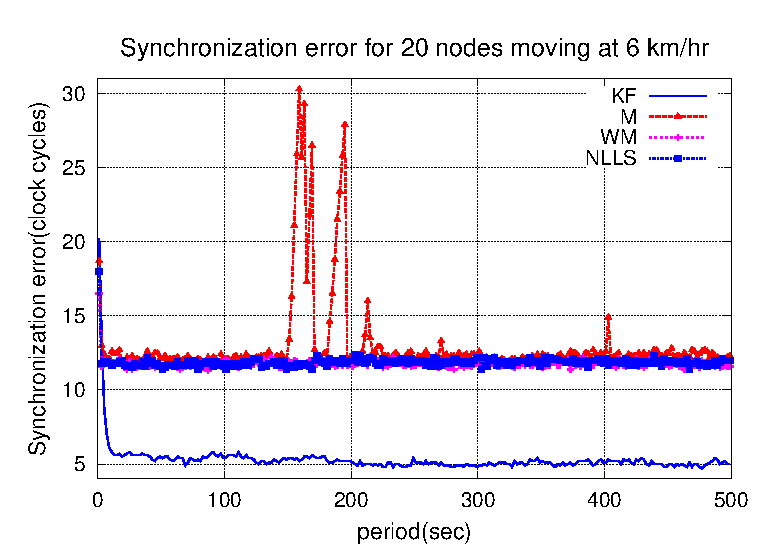
\includegraphics[width=0.7\textwidth]{16output-s6}
\caption{Synchronization error for 20 nodes - Speed 6km/hr} \label{16output6}
\end{figure}
In all cases the speed of the nodes is taken to be an independent Gaussian random variable with mean 20$km/hr$ and standard deviation $1km/hr$. The simulation results is presented, Figure $\ref{16output20}$. With the increase in the speed of the nodes, the precision of the algorithms improves. KF, with an average of of $10 clk$ performs the best, whereas WM and NLLS perform well too compared with the median, $1 clk$ and $1 clk$ respectively. As the dynamics of the networks increases, Median starts to have large deviations whereas NLLS and WM have a more stable performance.
\newline
The relative comparison of the algorithms performance improvement with the Median is shown in Figure $\ref{16error}$. WM and NLLS perform, on average, $6-8\%$ better than Median. The best performer, KF, has on average $60\%$ better performance than the Median one.
\begin{figure}
\centering
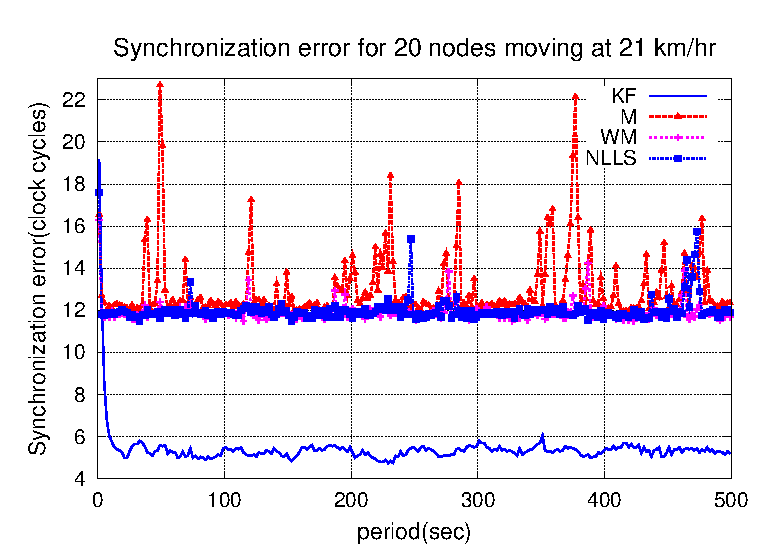
\includegraphics[width=0.7\textwidth]{16output-s20}
\caption{Synchronization error for 50 nodes - Speed 20km/hr}
\label{16output20}
\end{figure}
\subsubsection{\textbf{Case III}}
In this set of simulations, the number of the nodes is increased, to $50$. With slowly moving nodes ($6km/hr$), the results are shown in Figure $\ref{50output6}$. Large disruptions occur when using Median due to nodes moving slowly in the surrounding (leave the network and join again after some time), resulting in a larger drift with neighbors before getting back to the network. NLLS and WM perform better when it comes to stability. KF has the edge, both in precison and stablity.
\newline
\begin{figure}
\centering
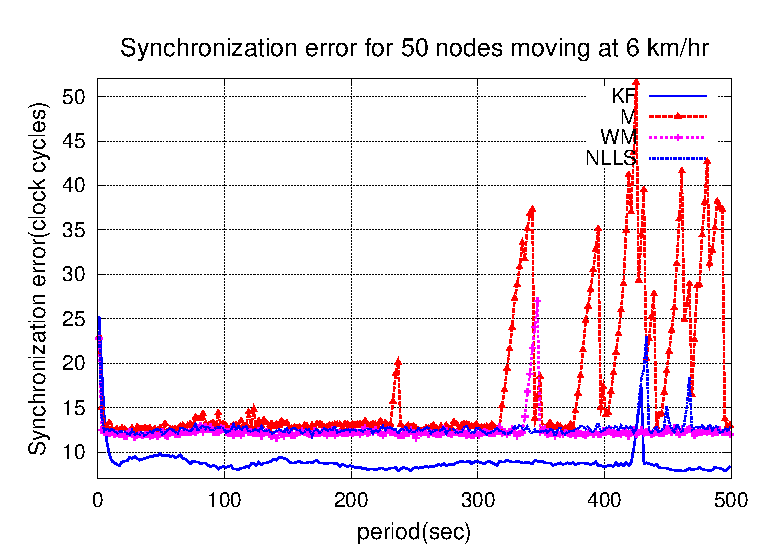
\includegraphics[width=0.7\textwidth]{50output-s6}
\caption{Synchronization error for 50 nodes - Speed 6km/hr}
\label{50output6}
\end{figure}
With a speed of $20km/hr$, the simulation result is presented in Figure $\ref{50output20}$. With this speed, the performance is
better due to the faster moving nodes, joining the networks at a faster rate. This helps in getting synchronized with the nodes in a
faster time, without drifting away for a longer period of time(which is the case in the first set of nodes with speed of $6km/hr$).
Again, for the set of nodes with a higher speed , a relative comparison is made to see the performance of the nodes with the
median algorithm.\newline
The Median algorithm is shown to perform the worst in this case. There are a lot of disruptions in the network, making it more unstable whereas the other algorithms adapt to the changes faster.
\newline
Figure $\ref{50error}$ shows that KF performs the best against Median algorithm, $45\%$. WM and NLLS perform well against Median too, $5\%$ on average. It has been shown that the median is prone to error in case of high dynamics in the network.
\begin{figure}
\centering
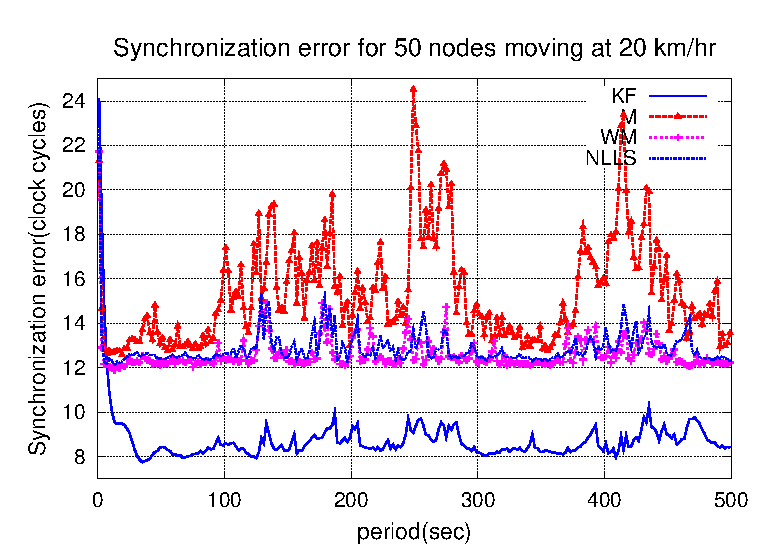
\includegraphics[width=0.7\textwidth]{50output-s20}
\caption{Synchronization error for 50 nodes - Speed 20km/hr} \label{50output20}
\end{figure}
\newline
In general, the Kalman Filter has a better precision and more stability than the rest whereas WM and NLLS are more stable than the Median.
\section{\textbf{Energy consumption}}
\begin{figure}
\centering
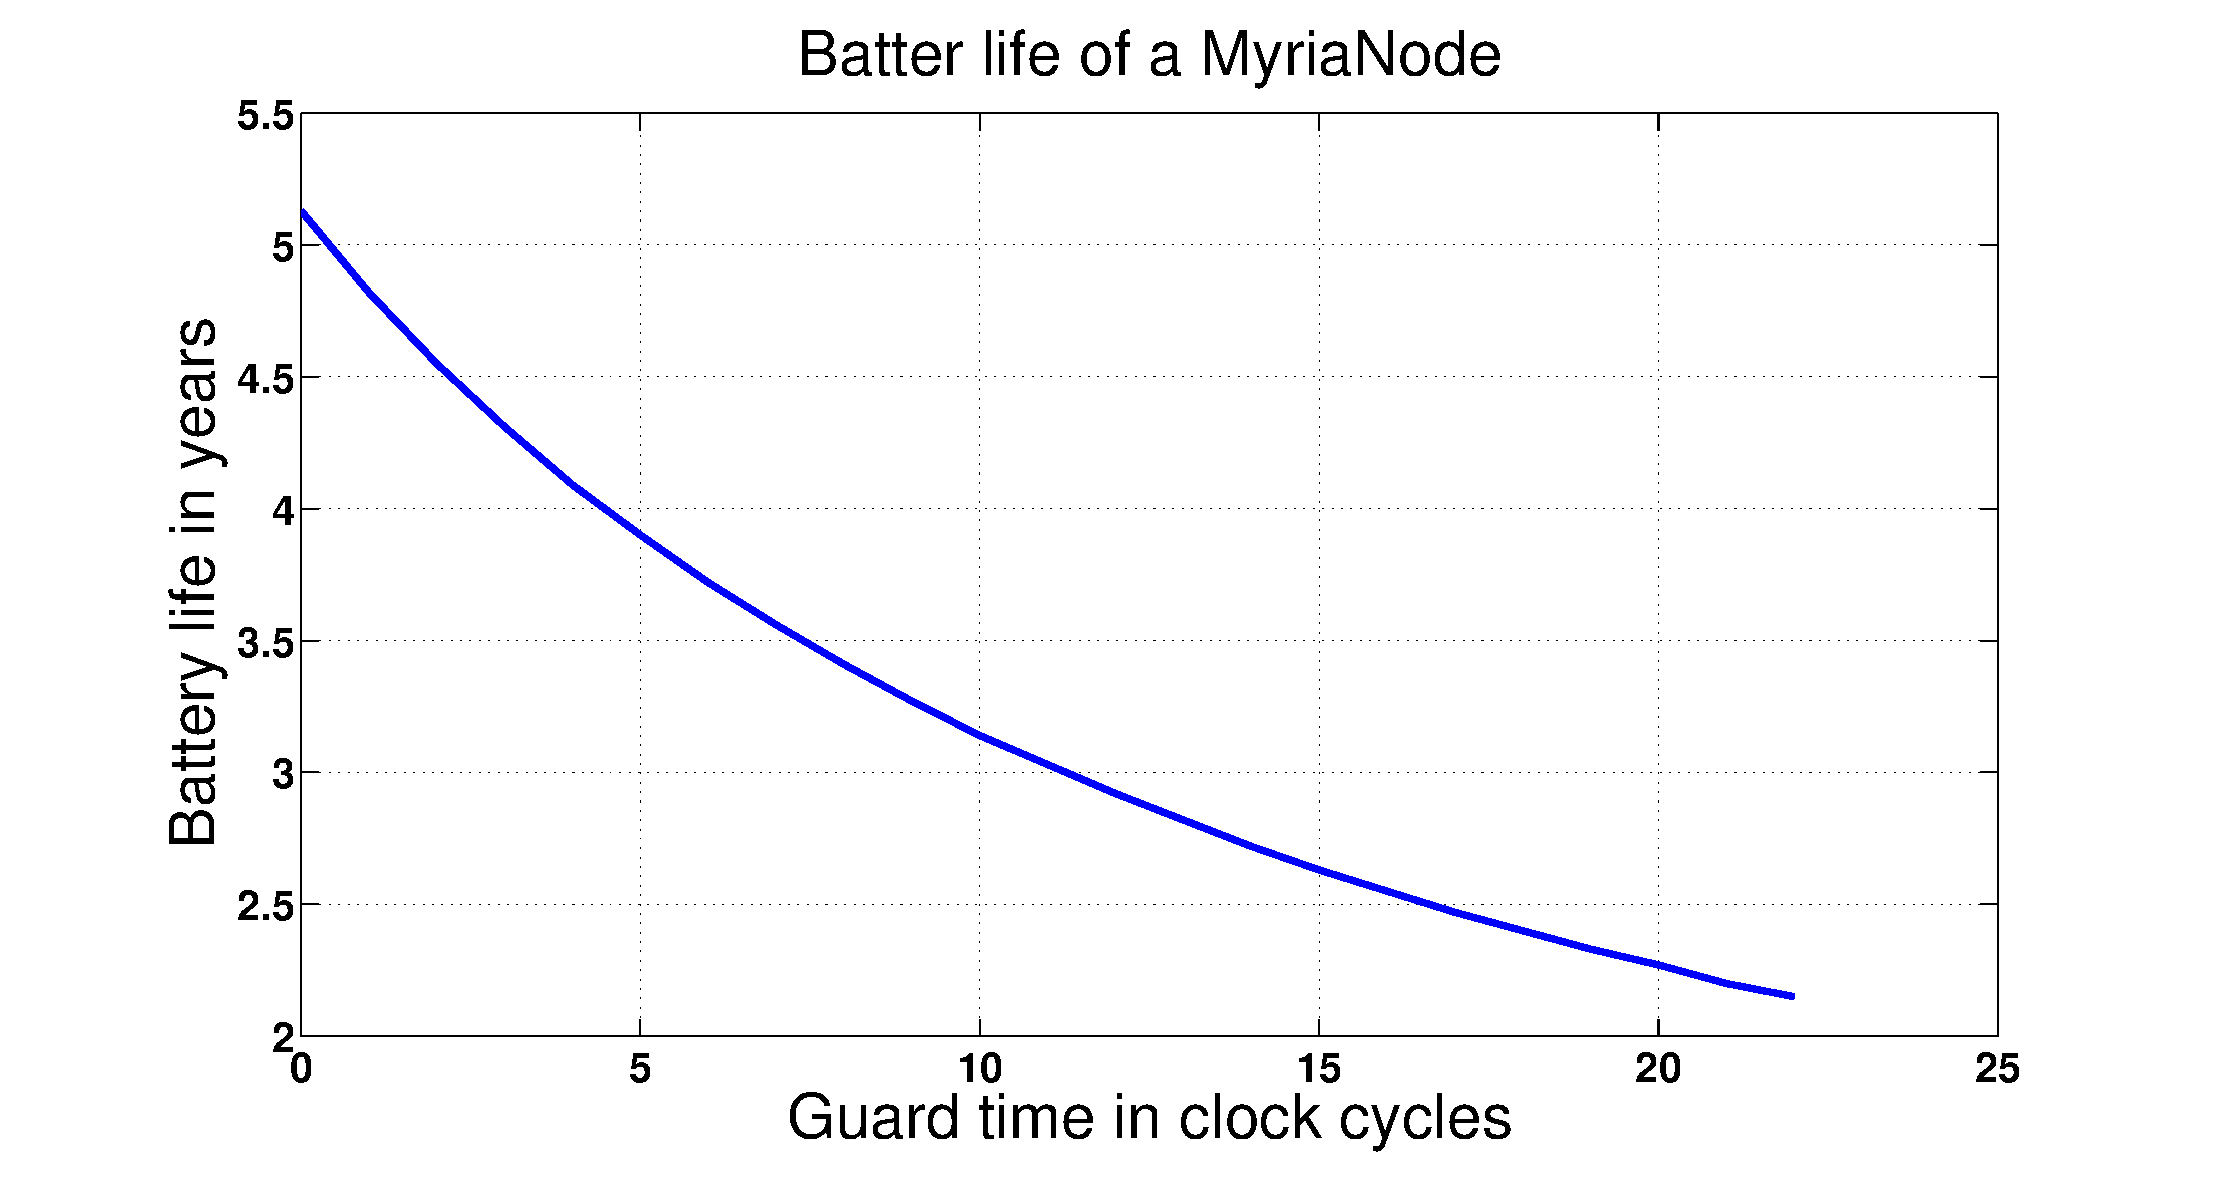
\includegraphics[width=0.7\textwidth]{guardsave}
\caption{The energy consumption of Guard time per RX slot}
\label{guardsave}
\end{figure}
As the results in the previous section shows, KF algorithm performs well in all conditions, so do WM and NLLS. The downside in
implementing these algorithms, despite the performance gain that all have against the Median is the energy consumption. As the algorithms are going to be implemented on the sensor nodes, the energy consumption is a priority in the study of embedded system algorithm development. The algorithms are written in C and implemented on the test nodes to see the effect that they are going to have on the energy consumption of the nodes.
\begin{center}
    \begin{tabular}{ |p{2cm} | p{4.75cm} |}
    \hline
    Algorithm & Average Execution Time \\ \hline
    M &  65 $\mu$s \\ \hline
    NLLS & 82.5 $\mu$s \\ \hline
    WM &   90 $\mu$s \\ \hline
    KF &  195 $\mu$s  \\ \hline
    \end{tabular}
\label{tab}
\end{center}
The table shows the average execution time of the algorithms in comparison to implemented on the MyriaNode. This doesn't show the
exact energy consumption of the algorithms but it can give us an approximation on the relative comparison of the algorithms about the energy consumption on the MyriaNode. As the table shows, the consumption of WM is 5$\%$ higher than the median algorithms. This
is also true for NLLS and KF which consume 9$\%$ and 4 $\%$ higher than the median algorithm respectively.
\newline
In order to reduce the energy that is going to be spent on the algorithm with a better performance, the guard time of the slot can be reduced, due to a better performance showing by KF, WM and NLLS. The energy consumption of the guard time is shown in Figure
$\ref{guardsave}$. The length of the guard time has a close-to-linear relation with the power being consumed in listening to the channel.
Thus, with the performance gain obtained, the guard time of the slot can be decreased, hereby decreasing the energy consumption of the node in general. Hence, by decreasing the guard time in proportion with the performance enhancement, we can save energy for the energy demand of the algorithm. This energy save is in a per slot basis. As the number of slots increases, the energy to be saved increases.
\chapter{\textbf{Conclusion and Recommendation}}
\section{\textbf{Conclusion}}
A decentralized frame synchronization of a TDMA-based WSN is achieved using Weighted Measurements (WM), Non Linear Least Squares(NLLS) and Kalman Filter (KF) methods. A simulation is conducted with different scenarios, especially taking the effect of mobility. A comparison of the algorithms with the currently implemented Median algorithm is conducted and the results are presented.
\newline
In a static environment, the KF performs the best whereas the WM and NLLS have shown a similar performance as the Median. In terms of convergence time, all have shown a similar performance.
\newline
A $60\%$ improvement in the performance of the synchronization can achieved on average using the Kalman Filter for dynamic WSN. A lower improvement, $8\%$ and $6\%$ is obtained using WM and NLLS methods for the synchronization of TDMA frames. Both WM and NLLS show a better tolerance against Median in a dynamic network. KF estimation of the next wake up time is the best with its iterative capability and adaptive nature.
\newline
Using these algorithms for a TDMA-based WSN synchronization( WM, NLLS and KF), the precision of the network increases. This in turn has a positive impact on the network because the synchronization period, $T_{sync}$ can be increased or the guard time of the node's frame, $t_{guard}$ can be reduced to achieve the same performance as the Median algorithm. Results are presented for an increased synchronization frequency.
\newline
But in the downside, the energy consumption of the algorithms is greater than the Median algorithm's energy consumption as the algorithms are more complex computationally. Analysis is made and presented about the energy saving made by decreasing the guard time of the slot. As shown in the measurements and analysis results, communication is around 5 times costlier than computation, on average. A net gain of battery life can thus be achieved by reducing the guard time.
\newline
Median is shown to be still the best choice in a static environment with the current implementation,with less energy consumption and simplicity into consideration. But, for dynamic networks, the other algorithms perform better, in terms of performance. KF has the edge due to its adaptive nature.
\section{\textbf{Recommendation}}
There are some suggestions on the future work of the algorithms.
\begin{itemize}
 \item
Upon the completion of the ongoing project on developing a Software Defined Radio (SDR) for the inspection of the nodes' wake-up times,
a proper evaluation and enhancements on the algorithms, being implemented on the MyriaNodes, is achievable. Real time feedbacks
can be used to improve the algorithms towards perfection.
\item
As KF is shown to have the best performance, different software power minimization techniques can be applied to further reduce the
power consumption of the algorithm implementation, making it more attractive for implementation. \item As it is shown in Section 3, the main sources of error for the clock inaccuracies are identified. Hence, solving the problem at its source is one approach which can be cost
effective as well as simple in implementation. This can be achieved using the available resources like the temperature sensor in the
microcontroller of the MyriaNode.
\end{itemize}
\appendix
\chapter{Simulation Results}
\section{\textbf{Median as a synchronization method}}
The performance of Median algorithm is dependent on the gain factor used in the offset calculation. Figure $\ref{gainfactor}$ shows the performance of the Median algorithm for different gain factors.
\begin{figure}[!h]
\centering
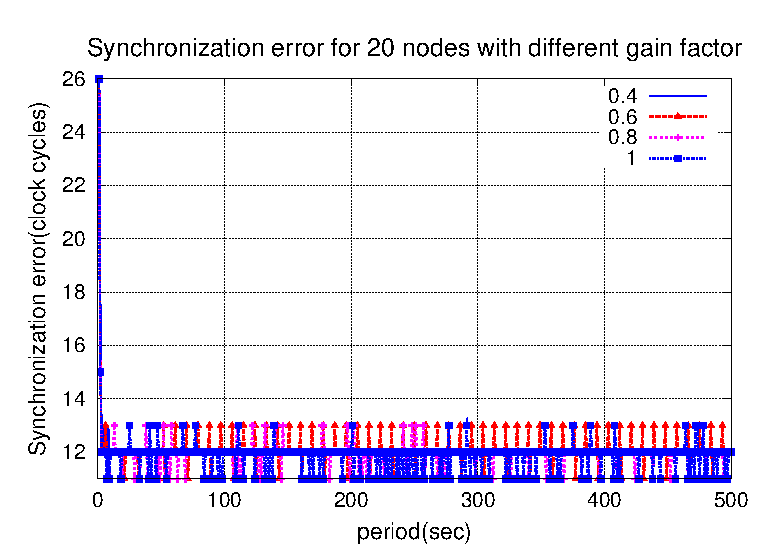
\includegraphics[width= 0.7 \textwidth]{gainfactor}
\caption{Median algorithm with different gain factors} \label{gainfactor}
\end{figure}
\section{\textbf{Synchronization frequency}}
Increasing the synchronization frequency increases performance but the precision decrease. Simulation is conducted for different synchronization frequency $T_{sync}$ on the KF algorithm. The simulation is conducted for different speeds, ranging from static nodes to nodes moving at a speed of around 20$km/hr$.
\newline
Figure $\ref{tsync0}$ shows the performance of KF with varying the synchronization frequency $T_{sync}$ for static nodes. Figure $\ref{tsync6}$ and Figure $\ref{tsync20}$ shows the performance of KF at different speeds, 6$km/hr$ and 20$km/hr$ respectively.
\begin{figure}[!h]
\centering
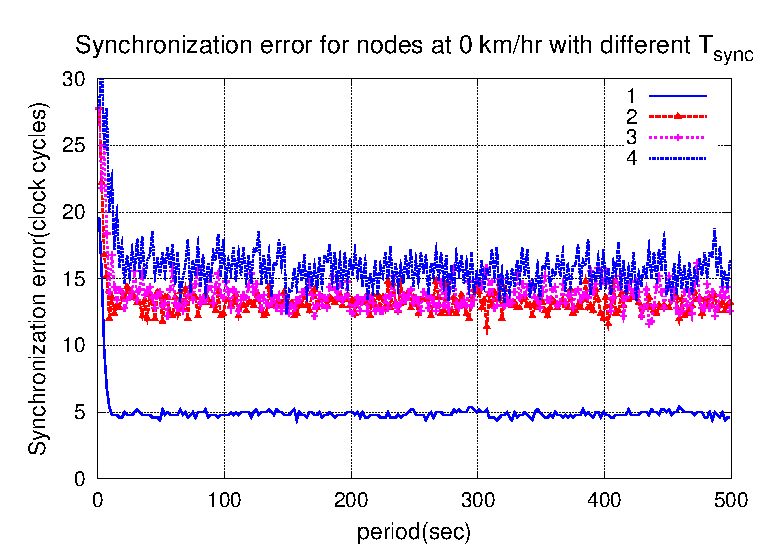
\includegraphics[width= 0.7 \textwidth]{tsync0}
\caption{Synchronization error of a KF for static nodes with different $T_{sync}$} \label{tsync0}
\end{figure}
\begin{figure}[!h]
\centering
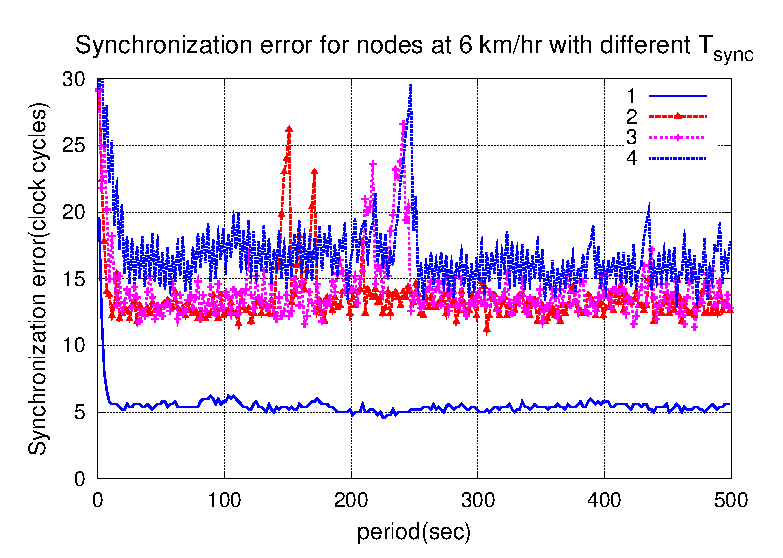
\includegraphics[width= 0.7 \textwidth]{tsync6}
\caption{Synchronization error of a KF for nodes at 6$km/hr$ with different $T_{sync}$} \label{tsync6}
\end{figure}
\begin{figure}[!h]
\centering
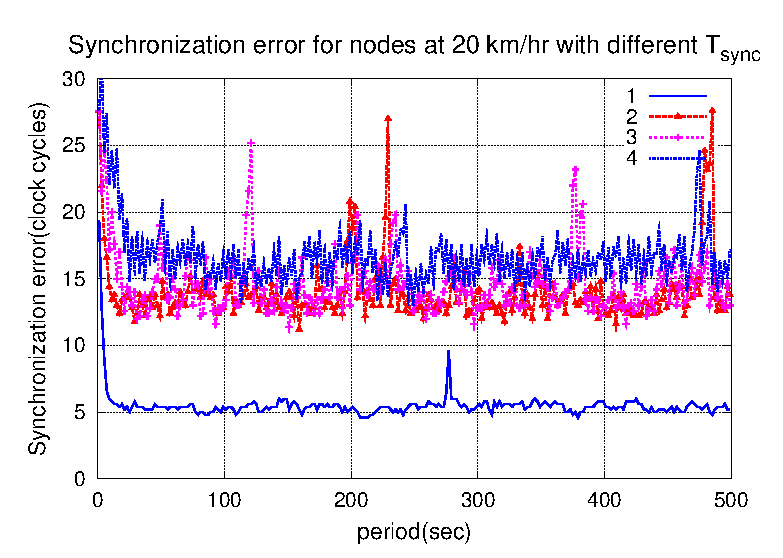
\includegraphics[width= 0.7 \textwidth]{tsync20}
\caption{Synchronization error of a KF for nodes at 20$km/hr$ with different $T_{sync}$} \label{tsync20}
\end{figure}
\section{\textbf{Synchronization error for nodes with different speeds}}
The synchronization error for nodes travelling with different speeds is given in Figure $\ref{varspeed16}$ for 20 nodes. For 50 nodes, the simulation result is shown in Figure $\ref{varspeed50}$. In both cases, KF performs the best out of all the algorithms.
\begin{figure}
 \centering
 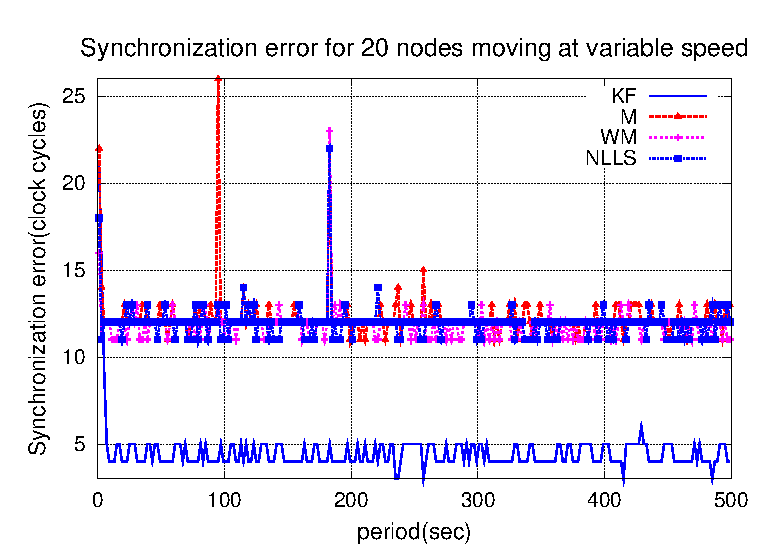
\includegraphics[width=0.6\textwidth]{varspeed20}
 \caption{Synchronization error for 20 nodes moving at different speed}
 \label{varspeed16}
\end{figure}
\begin{figure}
 \centering
 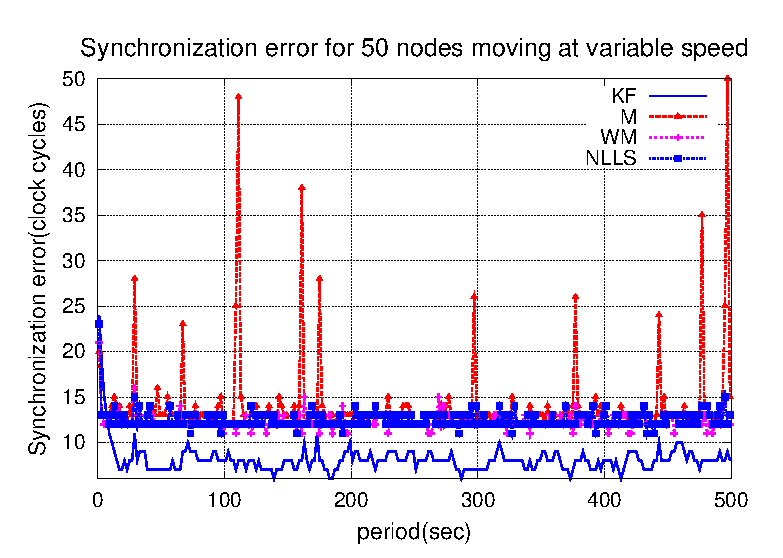
\includegraphics[width=0.6\textwidth]{varspeed50}
 \caption{Synchronization error for 50 nodes moving at different speed}
 \label{varspeed50}
\end{figure}
\section{\textbf{Relative performance improvement of the algorithms}}
The performance of the algorithms is compared with that of the Median. For 20nodes, see Figure $\ref{16error}$.
\begin{figure}[!h]
\centering
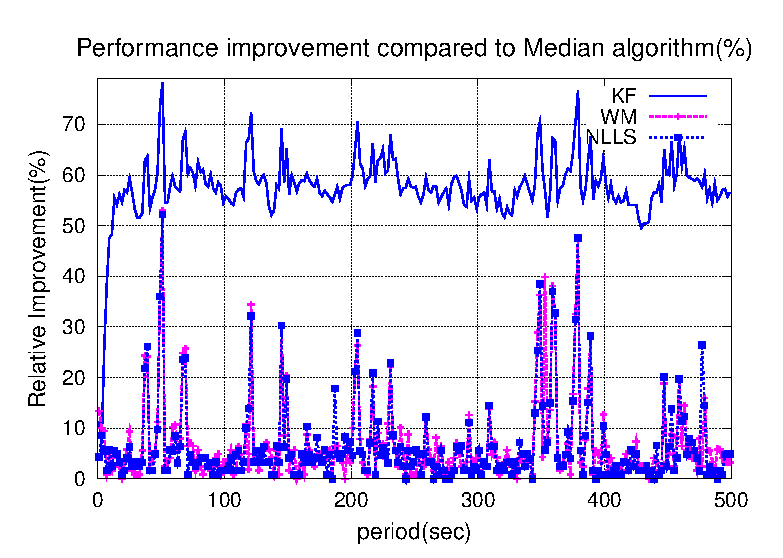
\includegraphics[width= 0.7 \textwidth]{16output-error}
\caption{Relative performance improvement of algorithms from Median - 20 nodes} \label{16error}
\end{figure}
The performance of the algorithms is compared with that of the Median. For 50 nodes, see Figure $\ref{50error}$.
\begin{figure}[!h]
\centering
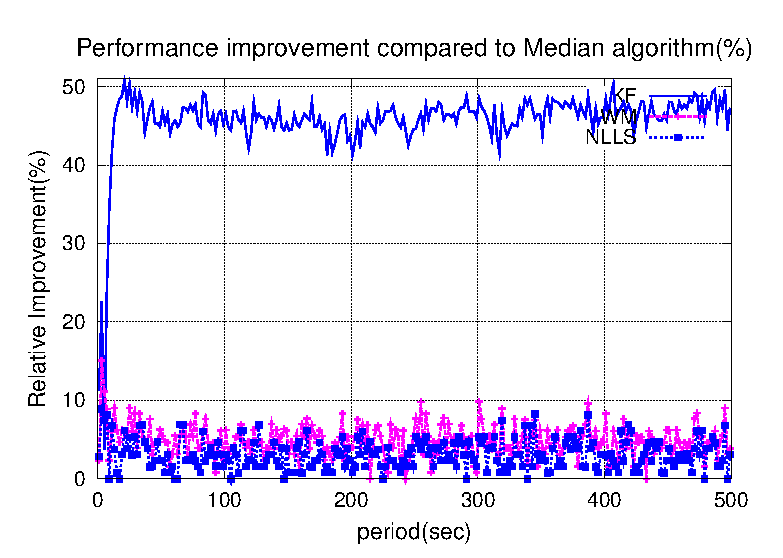
\includegraphics[width=0.7  \textwidth]{50output-error}
\caption{Relative performance improvement of algorithms from Median - 50 nodes} \label{50error}
\end{figure}
\chapter{MyriaNode}
\begin{figure}[!h]
 \centering
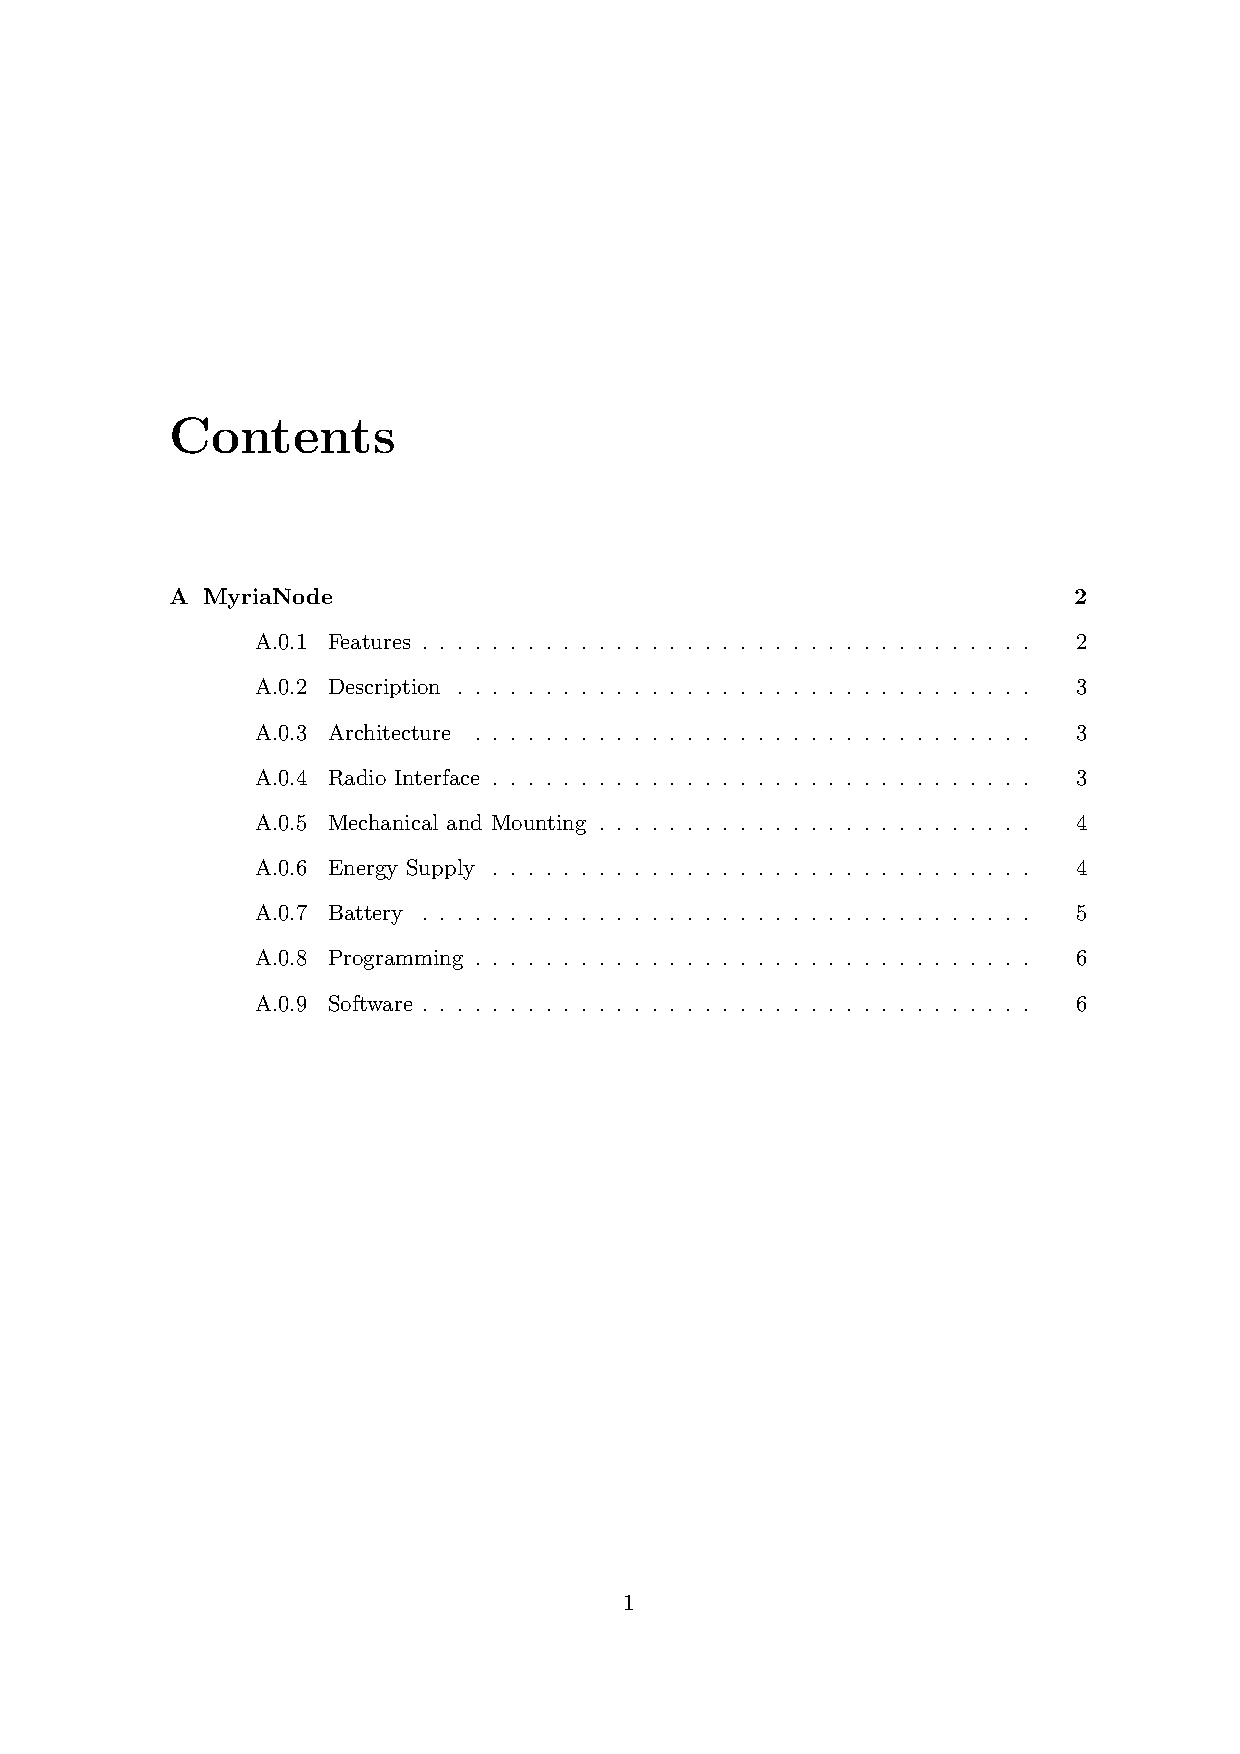
\includegraphics[width=0.5 \textwidth]{myrianode}
\caption{MyriaNode v2.0}
\label{myrianode}
\end{figure}
\subsubsection{Features}
\begin{itemize}
 \item 2.4 GHz ISM band
 \item Nordic nRF24L01 Radio
 \item Integrated 1/4$\lambda$ PCB antenna
 \item ATMega645 processor
 \item 64kB FLASH
 \item 4kB SRAM
 \item 2kB EEPROM
 \item 32kHz Crystal clock
 \item Size: 20 X 40 mm
 \item Single supply voltage: 1.9V - 3.6V
\end{itemize}
\subsubsection{Description}
This Wireless Sensor Node is the second generation product for the MyriaNed project. It integrates a Nordic radio module, antenna and embedded processor all on a PCB. The module is equipped with the software modules as they are being developed by one or more of the working groups of MyriaNed.
\subsubsection{Architecture}
\begin{figure}[!h]
 \centering
 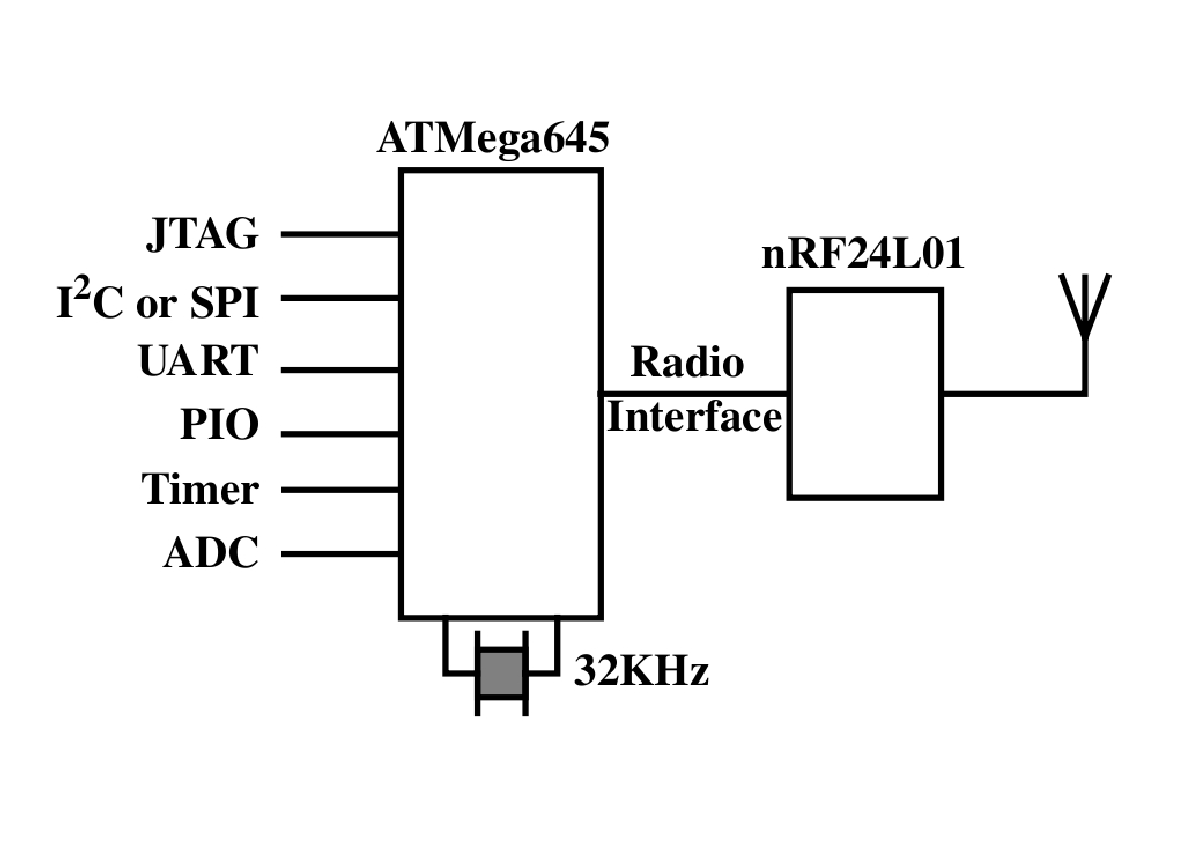
\includegraphics[width=0.5 \textwidth]{myrianodearch}
\caption{MyriaNode Architecture}
\label{myrianodearch}
\end{figure}
\subsubsection{Radio Interface}
SPI is used as interface between the processor and the radio, with the following interconnections:
\begin{figure}[!h]
 \centering
 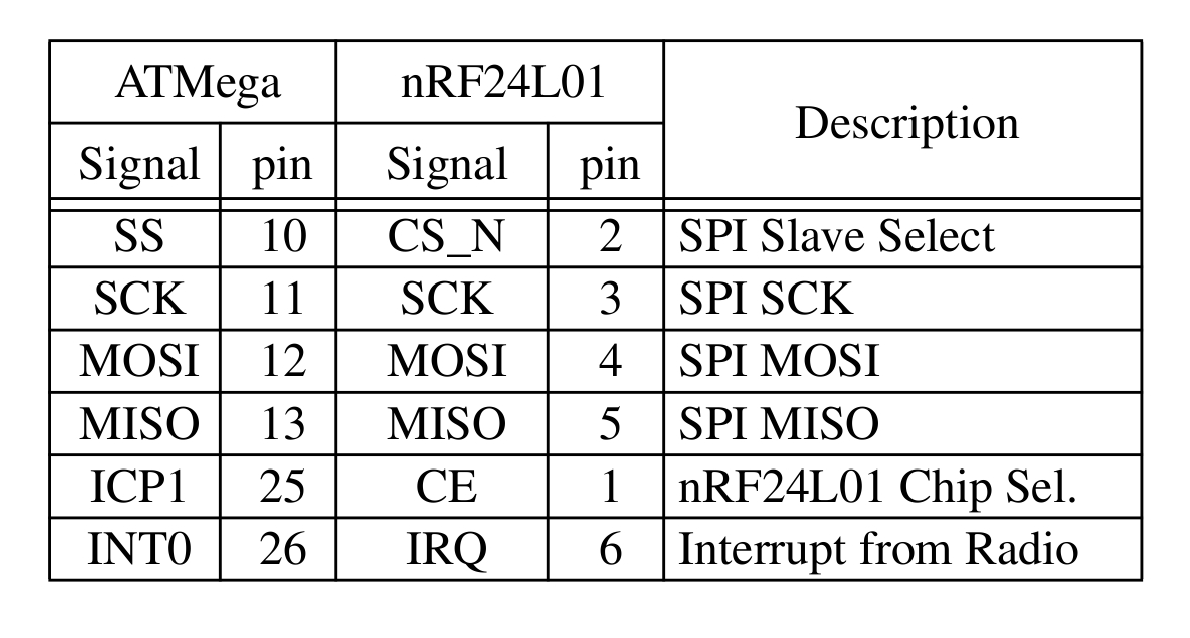
\includegraphics[width = 0.7 \textwidth] {table1}
 \caption{Radio Interface.}
 \label{table1}
\end{figure}
\newline
\begin{figure}[!h]
 \centering
 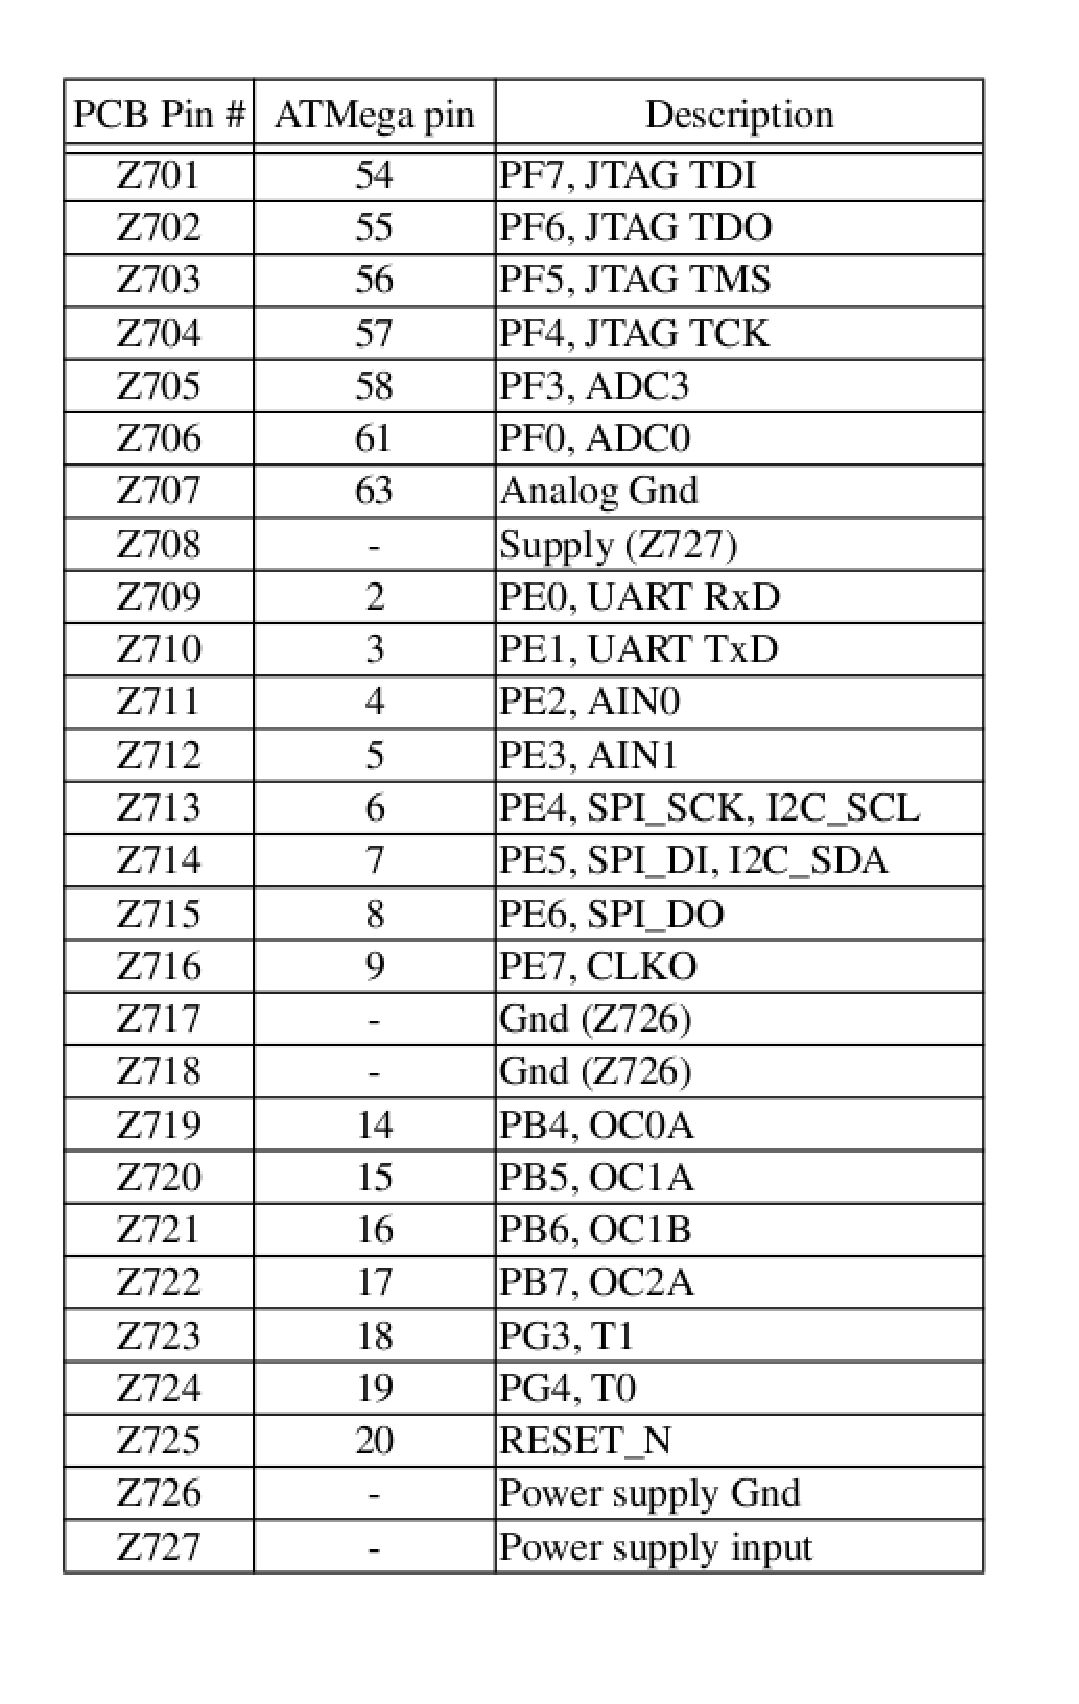
\includegraphics[width = 0.7 \textwidth] {table2}
 \caption{External interfaces.}
 \label{table2}
\end{figure}
\subsubsection{Mechanical and Mounting}
\begin{figure}[!h]
 \centering
 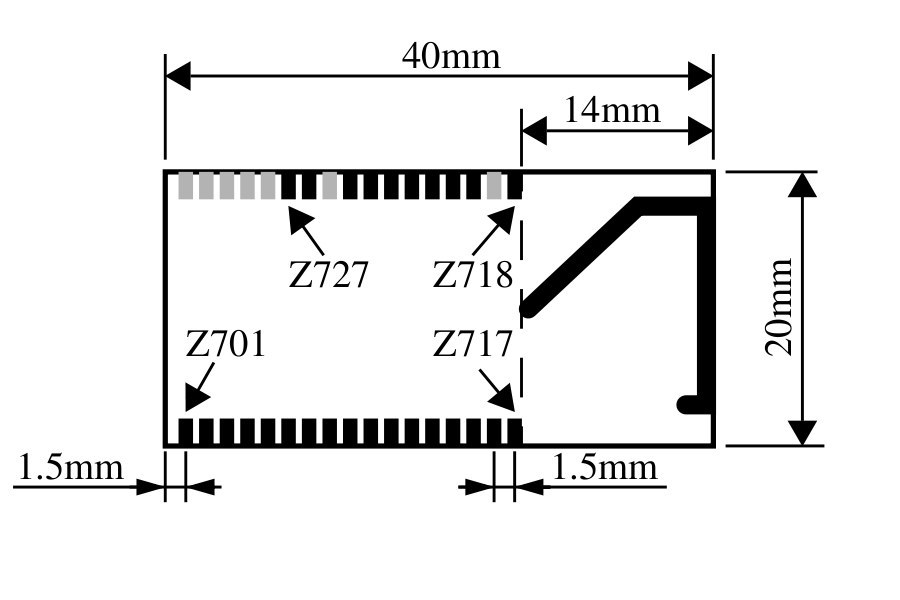
\includegraphics[width= 0.7 \textwidth]{myrianodephy}
 \caption{MyriaNode dimensions}
 \label{myrianodephy}
\end{figure}
Figure $\ref{myrianodephy}$ shows the top (component) view of the module. It can be mounted as a Surface Mount Device (SMD) directly onto a base PCB. The antenna area must be positioned in free air.
\subsubsection{Energy Supply}
Both the embedded processor and the radio are connected to the same supply rail. The supply voltage must therefore remain in a range that meet the supply voltage specifications of both devices, which is: 1.9V - 3.6V. \newline
In order to reduce conversion noise of the ADC to a minimum, the power decoupling circuit is implemented following the guidelines in the datasheet of the ATMega645. \newline
The energy consumption very much depend es on the network parameters and application software. Under average conditions of a network cycle time of 1s, and a frame size of 32 bytes, the node can last for at least 5 years on a Lithium Thionyl Chloride battery of 900mAh. \newline
The voltage level of a new Lithium Thionyl Chloride battery is 3.67V, while the absolute maximum operating voltage of the nRF24L01 is 3.60V. This requires a voltage reduction circuit. The most simple one is to connect the node via a diode to the battery, as is shown in Figure $\ref{battery}$.
\begin{figure}[!h]
 \centering
 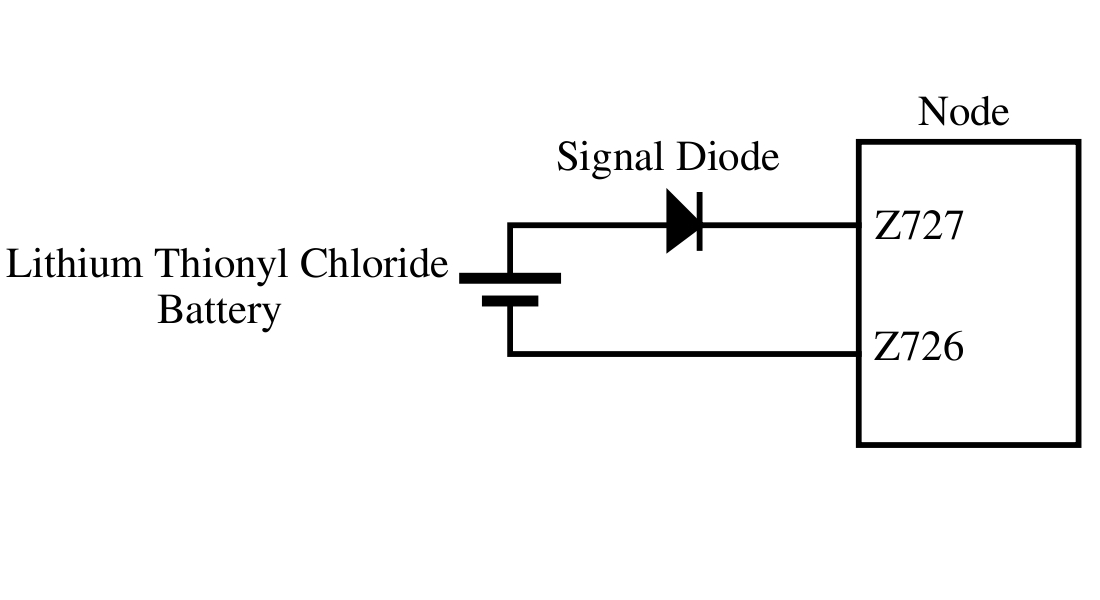
\includegraphics[width = 0.5 \textwidth]{battery}
 \caption{Battery structure of a MyriaNode}
 \label{battery}
\end{figure}
\subsubsection{Battery}
The ER14250STU from EMB is a Lithium Thionyl Chloride battery. It has a form factor of 1/2 AA size, and has a capacity of 1000mAh.
\subsubsection{Programming}
The node can be programmed and debugged via the JTAG interface. Although there are many second source suppliers of JTAG development tools, it is advised to use the AVR JTAGICE mkII from Atmel, ordering code: ATJTAGICE2.
\subsubsection{Software}
The software is documented by the other working groups of MyriaNed.
\begin{thebibliography}{\textbf{References}}
\bibitem{2}J.Elson, L.Girod and D.Estrin. Fine-grained network time synchronization using reference broadcasts. Proceedings of the 5th Symposium on Operating Systems Design and Implementation, Boston, Massachusetts, USA, December 9–11, 2002.
\bibitem{3}Q.Yang, and et al. A Decentralized Slot Synchronization Algorithm for TDMA-Based Ad Hoc Networks. Wireless Communications, Networking and Mobile Computing, 2007. Vol.21, Issue 25, Sept. 2007 pp.1717 - 1721.
\bibitem{mutualsync}E. Souour and M.Nakagawa. Mutual decentralized synchronization for intervechicle communications. IEEE Transactions and Vehicular Technology, Vol.48, Issue 6, pp.2015-2027.
\bibitem{4}A.Tyrrell, and et al. Firefly synchronization in ad hoc networks, in Proc. MiNEMA Workshop 2006, February, 2006.
\bibitem{5}NTP Public Services Project http://support.ntp.org/bin/view/Main/WebHome.
\bibitem{taxonomy}E.Anceaume and I.Puaut. A taxonomy of clock synchronization algorithms. IRISA Research Report No. PI1103, IRISA, 1997.
\bibitem{17}Q.Yang and J.Shi. An interference elimination method for decentralized slot synchronization in TDMA-based wireless ad hoc network. Intelligent Signal Processing and Communication Systems, 2007. Nov.28,2007-Dec.1,2007. pp.236-239.
\bibitem{pieter} P.Anemaet. Determining G-MAC potential with $\{$S,L,SCP$\}$-MAC. Masters thesis. Technische Universteit Delft. Delft. August 2008.
\bibitem{gossip}D. Gavidia, S. Voulgaris, and M. van Steen. A gossip-based distributed news service for wireless mesh networks. In Proceedings 3rd IEEE Conference on Wireless On demand Network Systems and Services (WONS), Les Menuires, France, January 2006.
\bibitem{6}R.John. Introduction to Quartz Frequency Standards. Technical Report SLCET-TR-92-1, Army Research Laboratory, Electronics and Power Sources Directorate. October 1992.
\bibitem{gradient}R. Fan and N. Lynch. Gradient clock synchronization. In Proceedings of the twenty-third annual ACM symposium on Principles of distributed computing (PODC ’04), pages 320–327. ACM Press, 2004.
\bibitem{gradient2}L.Meier,and L.Thiele. Gradient clock synchronization in sensor networks. Technical report, Computer Engineering and Networks Laboratory. Swiss Federal Institute of Technology Zurich, 2005.
\bibitem{7}J.Elson and D.Estrin. Time Synchronization for Wireless Sensor Networks. In Proceedings of the 15th International Parallel and Distributed Processing Symposium. IEEE Computer Society, April 23-27. 2001.
\bibitem{9}K.Romer. Time Synchronization in Ad Hoc Networks. In Proceedings of the Second ACM International Symposium on Mobile Ad Hoc Networking and Computing, Long Beach, California. 2001.
\bibitem{10}H.Karl and A.Willig. Protocols and Architectures for Wireless Sensor Networks.p3-6. Wiley. July 2006.
\bibitem{11}C.Cordeiro and D.Agrawal. Ad hoc and Sensor Networks Theory and applications. p.429-441. World Scientific Publishing. 2006.
\bibitem{1}F.Zhao and  L.Guibas. Wireless Sensor Networks: an Information Processing approach. p.107-108. Elsevier. 2004.
\bibitem{texas} S.Raje. Time synchronization of in Network-centric sensor networks. Master research. University of Texas, Arlington. Texas. August 2005.
\bibitem{14}S.PalChaudhuri and et al. Adaptive Clock Synchronization in Sensor Networks, Information Processing in Sensor Networks, April 2004.
\bibitem{correlation}A.Ebner, H.Rohling, M.Lott, and R.Halfmann. Decentralized Slot Synchronization in Highly Dynamic Ad Hoc Networks. Proc. WPMC '02, Honolulu, Hawaii, Oct. 2002.
\bibitem{16}G.Werner-Allen and et al. Firefly-inspired sensor network synchronicity with realistic radio effects. Proceedings of the 3rd international conference on Embedded networked sensor systems, San Diego, California. November 2005.
\bibitem{18} $http://www.golledge.co.uk/pdf/products/xtl\_sm/cc7v.pdf$
\bibitem{19} $http://pdfserv.maxim-ic.com/en/an/AN58.pdf$.
\bibitem{omnet}$http://www.omnetpp.org$.
\bibitem{kalm}$http://www.cs.unc.edu/~welch/kalman/$.
\end{thebibliography}
\end{document}
\textbf{``Unnecessary synchronization wastes resources; insufficient
synchronization leads to poor application performance.'' }
